% thesis?

\documentclass[mitthesis,12pt]{report}
\usepackage{baththesis}

\usepackage{amsmath, amssymb, amsfonts, url, natbib, bm, rotating, multirow, graphicx, psfrag, appendix}

 
% Shortcuts
% Probability
\newcommand{\prob}[1]{\mathbb{P}\left[ #1 \right]}
% fprime
\newcommand{\fprime}{f^\prime(z)}
% phi inverse
\newcommand{\phiinv}{\phi^{-1}}
% use other phi by default
\renewcommand{\phi}{\varphi}
%transpose
\newcommand{\tr}[1]{#1^{\text{T}}}
% diagonal
\newcommand{\diag}{\text{diag}}
% call \times \cross
\newcommand{\cross}{\times}
% shortcut for ij^{th}
\newcommand{\ijth}{$ij^{\text{th}}$}

% lazy citation correction...
\newcommand{\citeb}{\citet}
\renewcommand{\cite}{\citealp}

% references
% figure reference command
\newcommand{\fig}[1]{figure \ref{#1}}
% Figure reference command
\newcommand{\Fig}[1]{Figure \ref{#1}}
% table reference command
\newcommand{\tabref}[1]{table \ref{#1}}
% Table reference command
\newcommand{\Tabref}[1]{Table \ref{#1}}
% equation reference command
\newcommand{\eqn}[1]{(\ref{#1})}
% section references
\newcommand{\secref}[1]{section \ref{#1}}
\newcommand{\Secref}[1]{Section \ref{#1}}

\newcommand{\appref}[1]{appendix \ref{#1}}
\newcommand{\Appref}[1]{Appendix \ref{#1}}


% LaTeX laziness!
\newcommand{\bc}{\begin{center}}
\newcommand{\ec}{\end{center}}
\newcommand{\bn}{\begin{enumerate}}
\newcommand{\en}{\end{enumerate}}
\newcommand{\bi}{\begin{itemize}}
\newcommand{\ei}{\end{itemize}}
\newcommand{\be}{\begin{eqnarray}}
\newcommand{\ee}{\end{eqnarray}}
\newcommand{\bes}{\begin{eqnarray*}}
\newcommand{\ees}{\end{eqnarray*}}
\newcommand{\expect}[1]{\mathbb{E}\left[ #1 \right]}

% words
\newcommand{\sch}{Schwarz-Christoffel}
\newcommand{\tprs}{thin plate regression spline}

% whatever I call MDS+TP approach
\newcommand{\mdsap}{MDS+RS}
% whatever I call the MDS with duchon splines approach
\newcommand{\mdsds}{MSG}
% whatever I call the R package for this
\newcommand{\mdspack}{\texttt{mdspack}}

\title{Flexible models for statistical ecology}
\author{David Lawrence Miller}
\degree{Doctor of Philosophy}
\department{Department of Mathematical Sciences}
\degreemonthyear{August 2011}

\norestrictions

\begin{document}

\maketitle
\begin{abstract} 
This thesis is split into two parts:
\begin{enumerate}
	\item \textbf{Smoothing over complex regions}:
	\item \textbf{Mixture model detection functions for distance sampling}:
\end{enumerate}
\end{abstract}

%\newpage
%\begin{center}
%\vspace*{2in}
%\huge{AIEN API$\Sigma$TE$\Upsilon$EIN}
%\end{center} 

%\newpage
%\begin{center}
%\vspace*{2in}
%\huge{For $\mathcal{L}^*$.}
%\end{center} 

%\newpage{Acknowledgements}

\tableofcontents

\listoffigures

\listoftables

\chapter{An Introduction}
%\begin{quotation}
%``The major justification for the existence of any form of advanced voluntary organised education should be that it enables users to distort time and location in the learning process.'' 
%
%-- Cedric Price
%\end{quotation}

\label{chap-intro}

This chapter introduces the topics that will be addressed in the first six chapters regarding finite area smoothing. First, \secref{intro-GAM} gives an introduction to smoothing using splines in two dimensions, \secref{intro-extending} then discusses the larger class of models to which the smoothers belong, \secref{intro-inpractice} addresses some more practical issues, then finally \secref{intro-FAS} goes on to talk about existing approaches to spatial smoothing in a finite area.

\section{Smoothing in two dimensions using splines}
\label{intro-GAM}

In ecological studies, it is typical that one of the covariates collected is the location at which the sample has been taken. Two possible uses for such data are considered here. First, location may be the only covariate collected, in which case estimating the spatial distribution of the phenomena in question is the goal (usually by plotting some kind of surface as a function of geographical coordinates). Alternatively, the spatial covariates may be used to remove spatial autocorrelation from the data, making the effects of non-spatial covariates clear and thus improving inference.

The following two examples highlight these two different objectives:
\begin{enumerate}
\item Chlorophyl levels in the Aral sea are monitored using satellite images. Each pixel in the image represents an area of 9 kilometres square on the Earth. However, the satellite images are noisy and so adjacent pixels can have vastly different measured levels of chlorophyll. One would expect the levels to vary smoothly with location, so a model can be fitted to the image data which produces a smooth map of the chlorophyll concentration over the whole of the sea in an attempt to remove the noise. Figure \ref{aral-intro} shows both raw and smoothed chlorophyll levels in the Aral sea (these data are revisited in section \ref{aral-sec} and \ref{aral-revisit}).
\item We wish to model the distribution of the North sea whiting population through space and time. In particular numbers of fish of age one were recorded by pulling a net up through the water column at a set of sample points. The sample locations and dates were recorded along with sea surface temperature, the identity and nationality of the ship that took the measurement and the depth of the sea bed at the sample location. Such a model can be used to draw inference about how the population has changed over time (for example, to see if overfishing is a problem or perhaps to see if there are reporting discrepancies between ships). The whiting's distribution in space and time is non-homogeneous (in particular it is known that yearlings tend to be found close to the shore) and failing to model this spatial heterogeneity could introduce  bias in abundance estimates. Accurately modelling the spatial distribution is essential for reliable inference.
\end{enumerate}
In both of these examples it is assumed that the phenomena in question (chlorophyll concentration and whiting density) vary smoothly according to their spatial location in the sense that the trend surface does not have large jumps as location changes. In many situations this assumption is biologically plausible.

% Aral example
\begin{figure}[tb]
\centering
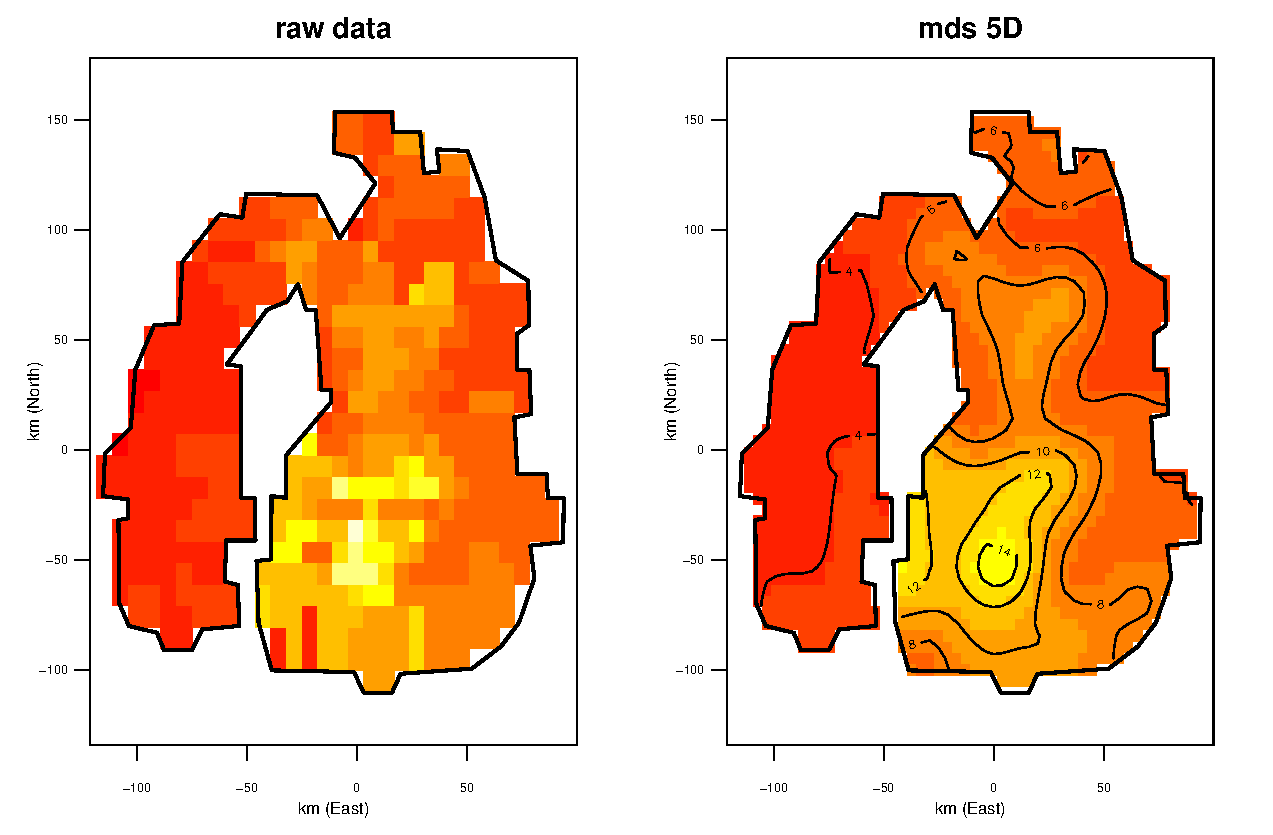
\includegraphics[width=\textwidth]{mds/figs/aral-5d-duchon.pdf}\\
\caption{Left: raw chlorophyll levels in the Aral sea as recorded by the SeaWIFS satellite. Right: a smoothed version of the data. Further analysis of the data may be found in sections \ref{aral-sec} and \ref{aral-revisit}.}
\label{aral-intro}
\end{figure}

There are many ways to construct models for the data described in the above examples, popular methods include kriging (\cite{diggle},  \cite{schabenberger}), kernel density estimation (\cite{wandKDE}) and hierarchical Bayes models (\cite{banerjee}). Here the focus is on using \textit{splines} (e.g. \cite{wahba}) for spatial smoothing via \textit{additive models} (e.g. \cite{gammonograph}).

Of particular interest here are smooth functions of space, and since the models are additive the emphasis is on situations akin to example 1 above, since if a method can be used in this context, it can also be included in models like those in example 2, simply as an additive component. For this reason, non-spatial covariates are ignored (for now).

Chapter 2 illustrates a situation akin to example 1 using administrative data from Italy and is based on the work in \citeb{miller2011}.

\subsection{Basic setup}
\label{intro-basic-setup}

First, denote observations of the phenomenon of interest as $z_i$ (in the examples above this would be the chlorophyll level or the yearling whiting catch at a particular point); $i$ indexes the samples $i=1,\ldots,n$, if there are $n$ samples . Each  $z_i$ is the realisation of some random variable $Z_i$, where $Z_i=\mu_i+\epsilon_i$, where $\mu_i=\mathbb{E}(Z_i)$, the expected value of the $i^\text{th}$ observation. Here $\epsilon_i$ is an error term and is assumed to be normally distributed with zero mean and some variance, $\sigma^2$. The spatial coordinates of the sample are also recorded, denote them $\mathbf{x}_i = (x_{i1}, x_{i2})$ (coordinates could be measured in latitude and longitude, or as kilometres North and East of some reference point, known as Northings and Eastings). The objective is to model the expected value of the response ($\mu_i$) using the coordinates at which the data were collected.

Assuming that the phenomenon of interest varies smoothly in space is equivalent to saying that $\mu_i$ varies smoothly in space. Letting $f$ be some smooth function, then as $\mu_i = f(\mathbf{x}_i)$:
\begin{equation*}
z_i = f(\mathbf{x}_i) + \epsilon_i.
\end{equation*}
The observations are a sum of a smoothly varying spatial component and some random error. The problem is now how to estimate $f$.

One can imagine several possible ways of obtaining a suitable $f$. For example, one might simply work through a large book of mathematical functions, estimating parameters and finding the function that would fit the data best (for some definition of ``best''). Alternatively one might estimate $f$ as a kind of moving average of the values (for example LOESS, \cite{loess2}). The first option seems extremely time consuming (if it were even plausible) and the second will not give an ``explicit'' functional form at the end to slot into other procedures later. Rather than use either of these, a \textit{basis function} representation is used for $f$. The idea is to build $f$ out of a sum of $J$ known functions, ($b_j$s, say) scaled by coefficients ($\beta_j$, say) and then estimate these coefficients rather than the function as a whole. Mathematically:
\begin{equation}
 f(\mathbf{x}_{i}) = \sum_{j=1}^J \beta_j b_j(\mathbf{x}_{i}).
\label{intro-basisdecomp}
\end{equation}
Now some care must be taken in choosing both how many $b_j$s are used ($J$) and their form. This is so that $f$ sufficiently flexible over the whole of the domain that is to be smoothed over. 

The next few sections present a brief introduction to how spatial smoothing using splines works, with a particular emphasis on the spatial case. However, it should be noted that at all times the models presented can be extended to higher (and lower dimensions) and that two dimensions are used for clarity and relevance. The primary references for the rest of this section are \citeb{simonbook} and \citeb{rwc}, both provide excellent complementary introductions to the topic.

\subsection{Smoothing with penalties}
\label{GAMpenalties}

If $f$ is very flexible it is possible that in estimating the $\beta_j$s an $f$ which tends toward interpolation of the data can be found. Interpolating the data is not useful since an $f$ that simply jumps from datum to datum does not say any more about the spatial distribution than merely looking at the data. To obtain an $f$ that interpolates the data, we can simply minimize the ordinary least squares (OLS) objective function. That is estimate the vector of coefficients, $\hat{\bm{\beta}}$, that minimizes:
\begin{equation}
\sum_{i=1}^n \left \{ z_i - f(\mathbf{x}_i) \right \}^2,
\label{intro-OLS}
\end{equation}
If the $b_j$s are a sufficiently rich set of functions, this objective function does nothing to stop $f$ simply interpolating the data (which would give a value of 0 in the above expression). To stop this from happening the ``wigglyness'' of $f$ is penalized.

Penalizing the \textit{wigglyness} (or \textit{roughness}, \cite{rwc}) of $f$ makes sense since (as stated above) the belief is that the underlying phenomena is smooth. Mathematically, taking (\ref{intro-OLS}) and adding on a penalty based on the wigglyness gives:
\begin{equation}
\sum_{i=1}^n \left \{ z_i - f(\mathbf{x}_i) \right \}^2 +  \lambda \int\int \lvert \lvert P f(\mathbf{x}) \rvert \rvert^2 \text{d}\mathbf{x}.
\label{intro-2d-objfcn}
\end{equation}
Here $P$ is some derivative operator, for example the second derivatives (e.g. $P=\left ( \frac{\partial^2}{\partial x_1^2}, \sqrt{2} \frac{\partial^2}{\partial x_1 x_2}, \frac{\partial^2}{\partial x_2^2}\right )$ in a 2-dimensional case). Integrating the derivatives over the whole space gives a measure of the wigglyness of the function, functions which vary a lot will lead to large values of the integral and hence have larger penalties. The exact form of $P$ changes with the basis and dimensionality of the problem (as will be seen in the next section).

Depending on the situation, the penalty should have a different amount of influence on (\ref{intro-2d-objfcn}). The \textit{smoothing parameter}, $\lambda$($\geq0$), controls the trade-off between interpolation (which happens as $\lambda \rightarrow 0$, leading to no penalty) and fitting a simpler function (which happens as $\lambda \rightarrow \infty$, where all terms are penalized aside from those for which the integral evaluates to zero: those in the \textit{nullspace} of the penalty). Figure \ref{lambda-ex} shows how different values of $\lambda$ affect the fitted smooth function. Determining the value of $\lambda$ will be covered in section \ref{GAMfitting}. For now it is assumed that some optimal $\lambda$ is known.

% example of setting lambda 
\begin{figure}[tb]
\centering
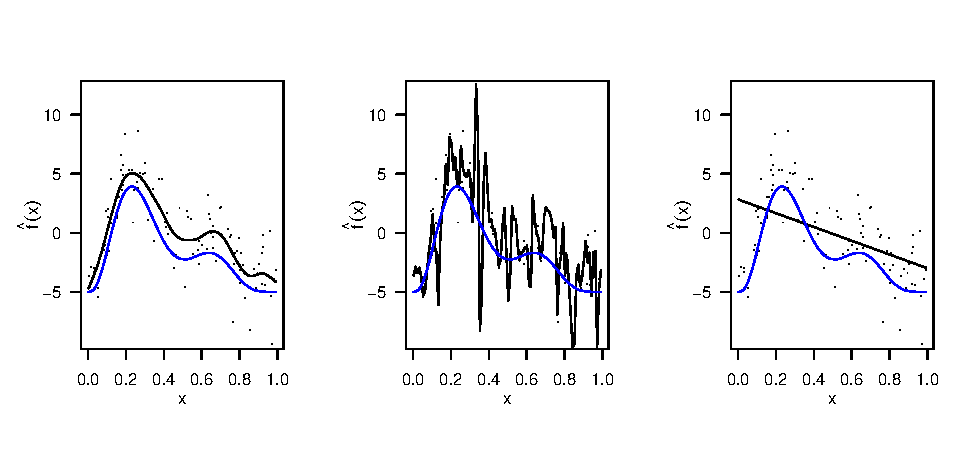
\includegraphics[width=6in]{intro/figs/lambda-ex.pdf}\\
\caption{An example of how different values of $\lambda$ affect the fitted smooth function of one variable. In the left panel, $\lambda$ is chosen optimally by GCV (see section \ref{GAMfitting}), in the middle panel $\lambda=0$, tending towards an interpolating fit. In the right panel $\lambda=\infty$ leading to a straight line. In each panel the blue curve is the true function and the points are the data sampled from it with error.}
\label{lambda-ex}
\end{figure}

The expression for the penalty given in (\ref{intro-2d-objfcn}) looks like it might require a rather large amount of integration and as such would require a long time to compute however, it can be shown (\cite[p. 128]{simonbook}) that the integral can be written as:
\begin{equation}
\int \dots \int \lvert \lvert P f(\mathbf{x}) \rvert \rvert^2 \text{d}\mathbf{x} = \bm{\beta}^\text{T} \mathbf{S} \bm{\beta},
\label{pen-quadform}
\end{equation}
where the $ij^\text{th}$ element of $\mathbf{S}$ is the integral of the product of the appropriate derivatives (in the above example, second) of the $i^\text{th}$ and $j^\text{th}$ basis functions. Put more mathematically:
\begin{equation*}
\mathbf{S}_{ij} = \int \dots \int \left(Pb_{i}(\mathbf{x})\right ) \left (Pb_{j}(\mathbf{x}) \right )^\text{T}  \text{d}\mathbf{x}.
\end{equation*}
So in this case the penalty matrix $\mathbf{S}$ only needs to be computed once. Computation of the penalty is merely a case of calculating the quadratic form in (\ref{pen-quadform}).

\subsection{Spline bases}

So far all that has been said about the form of $f$ is that it can be decomposed into a series of basis functions. Three bases are discussed here: \textit{thin plate regression splines}, \textit{P-splines} and \textit{cubic splines}, which will be used in this thesis.

\subsubsection{Thin plate regression splines}
\label{GAMtprs}
\label{GAMtprspenalty}
\label{cor-tprs}

This section begins by discussing \textit{thin plate splines} before going on to describe a computationally efficient version of the basis (\textit{thin plate regression splines}) which will be used throughout the thesis. Thin plate splines are particularly useful in a spatial setting because they have a property known as \textit{isotropy}: all directions have a common smoothing parameter so wigglyness in the $x_1$ direction has the same weight in the penalty as in the $x_2$ direction (and so on through higher dimensions). This property is usually appropriate in a spatial setting, since there is nothing special about one geographical coordinate over another when it comes to the smoothness of the function to be fitted.

Thin plate splines were first proposed by \citeb{duchon77}. Duchon begins by presenting the following penalty:
\begin{equation}
J_{m,d} = \int \ldots \int_{\mathbb{R}^d} \sum_{\nu_1 + \dots + \nu_d=m} \frac{m!}{\nu_1! \dots \nu_d!} \left ( \frac{\partial^m f(x_1,\dots,x_d)}{\partial x_1^{\nu_1} \ldots  \partial x_d^{\nu_d}} \right )^2 \text{d} x_1 \ldots  \text{d} x_d,
\label{tprs-pen}
\end{equation}
where $m$ is the \textit{derivative order}, $d$ is the dimension of the data (in a spatial setting $d=2$) and the $\nu_1,\ldots,\nu_d$ terms simply ensure that derivatives are taken with respect to all the parameters in all of the necessary combinations.

Replacing the penalty in (\ref{intro-2d-objfcn}) with (\ref{tprs-pen}), the objective function is then:
\begin{equation*}
\sum_{i=1}^n \left \{ z_i - f(\mathbf{x}_i) \right \}^2 +  \lambda J_{m,d}
\end{equation*}
It can then be shown that this objective function is minimized by a function of the form:
\begin{equation}
f(\mathbf{x}) = \sum_{i=1}^n \delta_i \eta_{m,d}(r_i) + \sum_{j=1}^M \alpha_j \phi_j(\mathbf{x}),
\label{tprs-basis} 
\end{equation}
where $r_i=\lvert \lvert \mathbf{x}-\mathbf{x_i}\rvert \rvert$ (the Euclidean norm of $ \mathbf{x}-\mathbf{x_i}$) and the $\delta_i$s and $\alpha_j$ are parameters to be estimated. As in (\ref{intro-basisdecomp}), $f$ is decomposed into a sum of basis functions however, for a thin plate spline this summation is split into two parts: $M$ polynomials that act over the whole of the data (the $\phi_j$s) and a set of \textit{radial basis functions}, one centred at each datum (the $\eta_{m,d}$s). One can think of this as a global trend (in the 2-dimensional case, linear functions of the two coordinates) with extra flexibility provided by the radial basis functions.

The radial basis functions $\eta_{m,d}(r)$ are defined as:
\begin{align*}
\eta_{m,d}(r) =\begin{cases} \frac{(-1)^{m+1+d/2}}{2^{2m-1}\pi^{d/2}(m-1)!(m-d/2)!} r^{2m-d} \log(r) &\quad{\text{$d$ even,}}\\
\frac{\Gamma(d/2-m)}{2^{2m}\pi^{d/2}(m-1)!} r^{2m-d} &\quad{\text{$d$ odd.}}
\end{cases}
\end{align*}
where $\Gamma$ is the gamma function. The $\phi_j$s are $M=\left( \begin{smallmatrix} m+d-1 \\ d  \end{smallmatrix}\right)$ linearly independent polynomials of degree less than $m$ which span the space of polynomials in $\mathbb{R}^d$; all of the $\phi_j$s are unpenalized as they lie in the nullspace of the penalty. It is also important to note that to maintain continuity in $f$, $2m>d$; this means that the dimension of the nullspace increases rapidly with $d$ (this will be discussed further in chapter \ref{chap-gds}).

This all looks rather complex, however in the 2-dimensional case, (\ref{tprs-pen}) looks much simpler. Setting $d=2$ and $m=2$, (\ref{tprs-pen}) is given as:
\begin{equation*}
J_{2,2} = \int \int \left ( \frac{\partial^2 f(x_1,x_2)}{\partial x_1^2} \right )^2 + 2\left ( \frac{\partial^2 f(x_1,x_2)}{\partial x_1  \partial x_2} \right )^2 + \left ( \frac{\partial^2 f(x_1,x_2)}{\partial x_2^2} \right )^2 \text{d} x_1 \text{d} x_2,
\end{equation*}
and $f$ is:
\begin{equation*}
f(\mathbf{x}) = \sum_{i=1}^n \delta_i \eta_{2,2}(r_i) + \sum_{j=1}^3 \alpha_j \phi_j(\mathbf{x}),
\end{equation*}
where:
\begin{equation*}
\eta_{2,2}(r) = \frac{1}{8\pi} r^2 \log(r).
\end{equation*}
The nullspace of the penalty consists of three functions: $\phi_1(\mathbf{x})=1, \phi_2(\mathbf{x})=x_1 \text{ and } \phi_3(\mathbf{x})=x_2$, which make no contribution to $J_{2,2}$. Figure \ref{tprs-basis-fig} shows some examples of 2-dimensional thin plate basis functions.

% tprs basis fig
\begin{figure}[p]
\centering
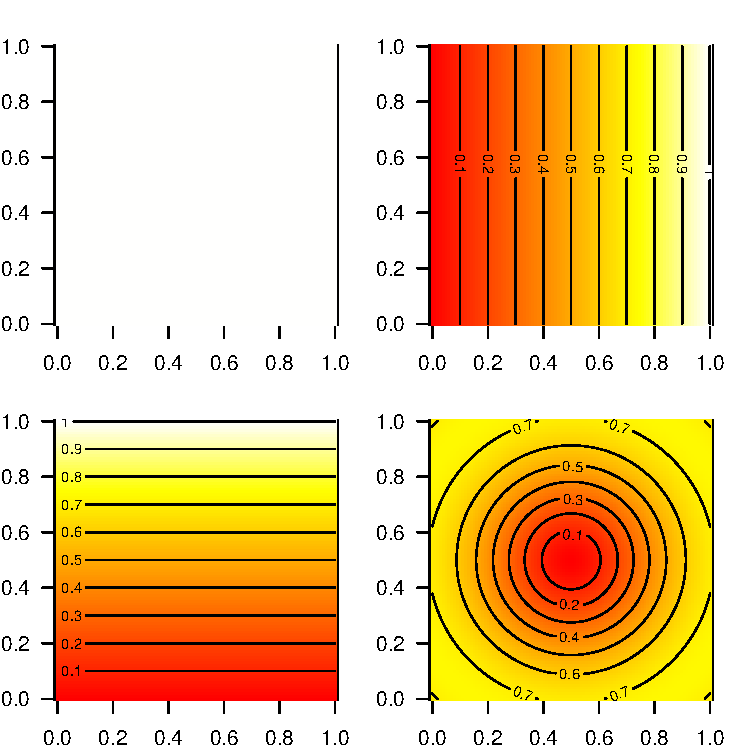
\includegraphics[width=\textwidth]{intro/figs/tprsex.pdf}\\
\caption{Example of a thin plate spline basis. The first three are $\phi_1(\mathbf{x})=1, \phi_2(\mathbf{x})=x_1 \text{ and } \phi_3(\mathbf{x})=x_2$, which are in the nullspace of the $J_{2,2}$ penalty. The bottom right plot shows an example of a radial basis function centred on $(0.5,0.5)$ with coefficient $-100$ (to put it on the same colour scale).}
\label{tprs-basis-fig}
\end{figure}

The computational cost of fitting the model is cubed in the number of parameters, so fitting a model with one radial basis function per datum may prove impractical in some cases. To avoid this problem, one could either ($i$) select (perhaps randomly) some of the data and use only those points to create the basis and then use the full data to fit the model (i.e. changing the index of the summation in the first term of (\ref{tprs-basis})) or ($ii$) select a (relatively small) representative set of points within the space covered by the data (though not necessarily data locations) which would be evenly spread out enough to create the basis (changing the $\mathbf{x}_i$s in the first summation in (\ref{tprs-basis}) -- these points are known as \textit{knots}). Both approaches have potential problems, namely: how many points should be chosen and where they should best be located? Both of theses approaches effectively reduce the size of the basis (changing the limit on the first summation in (\ref{tprs-basis})), however both methods do this in a fairly arbitrary way. There is no objective measure of whether the points selected are ``good''. 

\citeb{wood2003} proposes a low-rank approximation to thin plate splines, referred to in this thesis as \textit{thin plate regression splines}. Let the $ij^\text{th}$ element of the ($n \times n$) matrix $\mathbf{E}$ be the $j^\text{th}$ radial basis function evaluated at the $i^\text{th}$ datum (i.e. $\mathbf{E} = \eta_{m,d}\left (\vert\vert\mathbf{x}_i - \mathbf{x}_j \vert\vert \right )$), reducing the computations required to fit the model can be achieved by reducing the rank of $\mathbf{E}$. In the previous two approaches the rank reduction was performed by removing columns from $\mathbf{E}$ (randomly sampling the data) or changing the number of columns by changing the location of the evaluations (using knots). 

One way of reducing the size of $\mathbf{E}$ is by performing an eigen-decomposition (so $\mathbf{E}=\mathbf{U}\mathbf{\Lambda}\mathbf{U}^\text{T}$, where the columns of $\mathbf{U}$ are orthogonal eigenvectors and $\mathbf{\Lambda}$ is a diagonal matrix of eigenvalues decreasing in absolute value down the diagonal). Picking the $k$ largest eigenvalues and truncating at that point (taking the first $k$ columns of $\mathbf{U}$ and the top right $k\times k$ submatrix of $\mathbf{\Lambda}$) gives $\mathbf{E}_k(=\mathbf{U}_k\mathbf{\Lambda}_k\mathbf{U}_k^\text{T})$. It can be shown that the reduced rank matrix $\mathbf{E}_k$ gives the best approximation to $\mathbf{E}$ (see \cite{wood2003} for details). In practice, $k$ is set to be ``large enough'' and further reduction in basis complexity is performed by penalization (see \secref{GAMEDF}). In the simulations and analyses in the following chapters $k$ will be referred to as the ``maximum basis size'' to avoid confusion.

This low-rank approximation is the default implementation when using the ``\texttt{tp}'' basis in the \textsf{R} package \texttt{mgcv}. This package was used throughout the thesis.

\subsubsection{P-splines}
\label{intro-psplines}

P-splines (\cite{eilersmarx96}) consist of B-spline basis function with discrete penalties, so before thinking about P-splines, the properties of B-splines are considered. 

B-splines are simple local basis functions; they are simple in that all of the basis functions have the same shape and local in that they only have an effect near where they are centred (at the knots) -- \textit{compact support}. Taking (\ref{intro-basisdecomp}), we replace the $b_j$s with an $(m+1)^\text{th}$ order B-spline $B_j^m$ (where the order is chosen). Note that the $B_j^m$s are only a function of one covariate, $x$, at this point but will be expanded to higher dimensions below. So, the basis representation of $f$ given in (\ref{intro-basisdecomp}) becomes:
\begin{equation*}
f(x) = \sum_{j=1}^{J} \beta_j B^m_j(x).
\end{equation*}
The $B_j^m$s are defined recursively as:
\begin{equation*}
B_j^m(x) = \frac{x-x^*_j}{x^*_{j+m+1} - x^*_j} B_j^{m-1}(x) + \frac{x^*_{j+m+2} -x}{x^*_{j+m+2} - x^*_{j+1}} B_{j+1}^{m-1}(x) \quad \text{for } j=1,\ldots,J,
\end{equation*}
and
\begin{equation*}
 B_j^{-1}(x)=\begin{cases}
1 \quad x_j \leq x < x_{j+1}\\
0 \quad \text{otherwise}. 
\end{cases}
\end{equation*}
The $J+m+1$ knots $x^*_j$ are evenly spaced over the $x$-axis and these, along with the order of the basis, determine how flexible $f$ is. Each $B^m_j(x)$ is non-zero over the $m+3$ adjacent knots. Contrary to their rather complex functional form, the functions shown in figure \ref{bs-basis} are rather simple. From left to right the panels show B-splines bases with $m=1,2,3$ for evenly spaced knots over $(0,1)$.

% b-splines example 
\begin{figure}[tb]
\centering
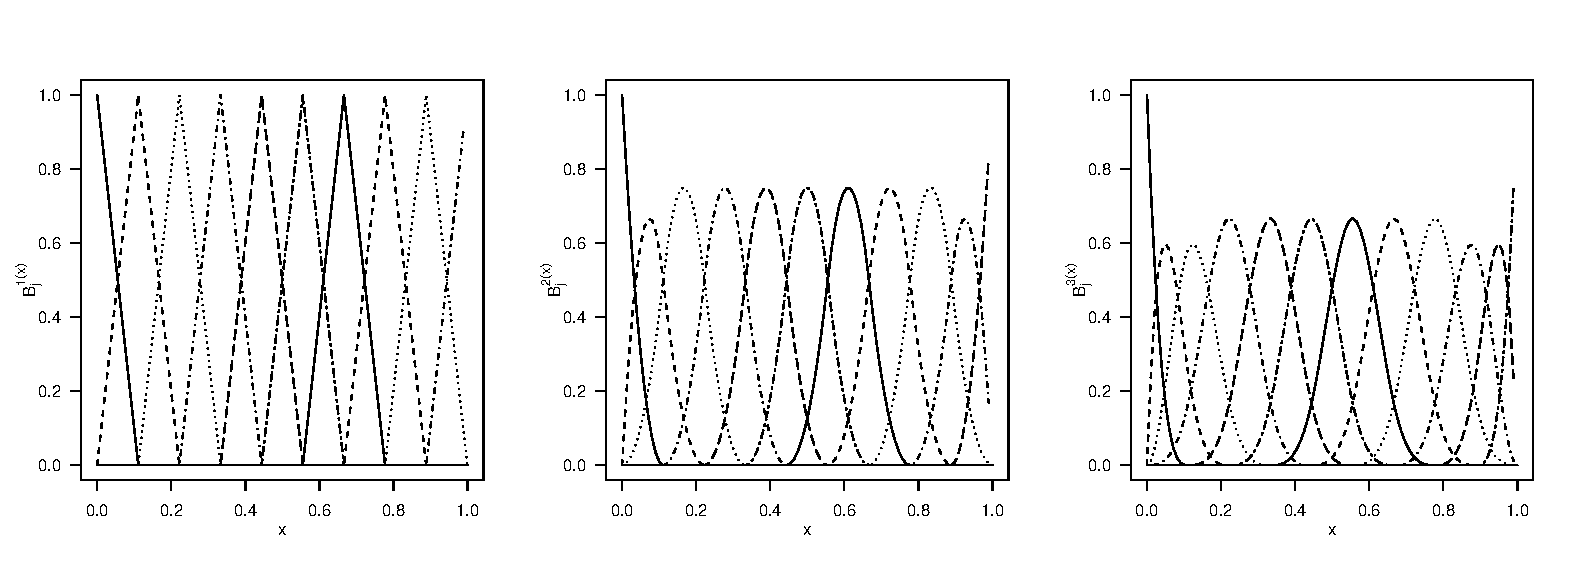
\includegraphics[width=\textwidth]{intro/figs/bspline-ex.pdf}\\
\caption{An example of B-spline basis functions for $m=1, 2$ and $3$ (from left to right) with evenly spaced knots (these are located at the peaks of the basis functions).}
\label{bs-basis}
% generated by phd-smoothing/thesis/intro/figs/bspline-ex.R 
\end{figure}

P-splines take the B-spline basis and add a penalty structure. Because of their local nature, the penalty is somewhat different to the general penalty in (\ref{intro-2d-objfcn}) and is based on differences between adjacent bases. Since the $B^m_j$s are defined locally, smoothness only needs to be enforced on neighbouring basis functions. The objective function given in (\ref{intro-2d-objfcn}) then becomes:
\begin{equation*}
\sum_{i=1}^n \left \{ z_i - f(x_i) \right \}^2 +  \lambda \sum_{j=1}^{J-1} (\beta_{j+1} - \beta_j)^2,
\end{equation*}
if squared second differences are used (this could be a higher order difference, see \cite{eilersmarx96}). Such a penalty is very fast to compute, since many of the elements of the penalty matrix, $\mathbf{S}$, are zero due to the local nature of the basis functions.


\subsubsection{Cubic splines}
\label{intro-cubic}
\label{cor-cubic}

\textit{Cubic splines} are another a univariate basis and, like P-splines they require the specification of knots. Cubic splines are made up of sections of cubic polynomials which are continuous (up to second derivatives) at the joins. The objective function for a cubic spline is:
\begin{equation*}
\sum_{i=1}^n \left \{ z_i - f(x_i) \right \}^2 +  \lambda \int_{x^*_1}^{x^*_J}\left( \frac{\partial^2 f(x)}{\partial x^2} \right)^2 \text{d}x,
\end{equation*}
where $\{x_j^* : j=1,\ldots,J\}$ are $J$ knots. This gives rise to the set of cubic polynomials that form the basis. Such a basis has many possible parametrizations; here the ``cardinal'' parametrisation is used (the basis functions take the value one at one knot and zero at all others). The parametrization gives the following form for $f$:
\begin{align*}
f(x) =& \frac{x_{j+1}^* - x}{x_{j+1}^* - x_j^*} \beta_j + \frac{x - x_j^*}{x_{j+1}^* - x_j^*} \beta_{j+1}\\
& + \left\{ \frac{\left (x_{j+1}^* - x\right )^3}{x_{j+1}^* - x_j^*} - (x_{j+1}^* - x_j^*)(x_{j+1}^* - x)\right \}\frac{\delta_j}{6}\\
& + \left\{ \frac{\left (x - x_j^*\right )^3}{x_{j+1}^* - x_j^*} - (x_{j+1}^* - x_j^*)(x - x_j^*)\right \}\frac{\delta_{j+1}}{6} \qquad \text{if } x_j^* \leq x \leq x_{j+1}^*.
\end{align*}
Letting $\beta_j = f(x_j^*)$ and $\delta_j = \frac{\partial^2 f(x)}{\partial x^2}\vert_{x=x_j^*}$, one can then write the $\delta_j$s as a function of the $\beta_j$s. Summing over $j$ then yields an implicit set of $J$ $b_j$s as in (\ref{intro-basisdecomp}). The cubic spline basis is then parameterized in terms of its values (and the values of its derivatives) at the knots. This setup may seem odd but does lead to the spline having directly interpretable parameters (which is not the case for, say, thin plate splines). An example of a basis function is given in figure \ref{cs-basis}.

Further details may be found in \citeb[pp. 122-126, pp. 149-151]{simonbook}.

% cubic example 
\begin{figure}[tb]
\centering
\includegraphics[width=0.5\textwidth]{intro/figs/cubic.pdf}\\
\caption{An example of a cubic spline basis function with a knot at 0.5. Figure taken from \citeb[p. 151]{simonbook}.}
\label{cs-basis}
% STOLEN! 
\end{figure}

\subsubsection{Cyclic cubic splines}

The above spline basis may be extended to a \textit{cyclic cubic spline} by imposing the constraint that $f(x_1)=f(x_k)$ and that the values of the first and second derivatives must also match. This specifies that the spline must ``join up'' at each end. The form of $f$ is the same as before, but there is one less coefficient to estimate (since the first and last are the same).

\subsubsection{Tensor products}
\label{GAMtensor}

Both P-splines and cubic splines are defined only in one dimension, however, it is possible to build 2-dimensional (and higher) smooths from \textit{tensor products} of 1-dimensional bases. This is made possible by thinking of each 1-dimensional basis as a marginal of the higher dimensional smooth. A spatial smooth of, say $x_1$ and $x_2$ can be constructed by first writing down the basis expansions for the marginal smooths of $x_1$ and $x_2$ (in general terms, since this applies to all splines not just P-splines and cubic splines, see \secref{3D}):
\begin{equation}
f_{x_1}(x_1) = \sum_{j=1}^J \beta_j b_j(x_{1}), \quad  f_{x_2}(x_2) = \sum_{k=1}^K \delta_k d_k(x_{2}).
\label{intro-tensor-def}
\end{equation}
where the $\delta_k$ and $d_k$ are analogous to $\beta_j$ and $b_j$ and assuming basis sizes of $J$ and $K$ (of course, $J$ and $K$ may be the same size). To make $f_{x_1}$ vary with $x_2$ we can then simply make the $\beta_j$s a function of $x_2$, the simplest way of doing this would be to define:
\begin{equation*}
\beta_j(x_2) = \sum_{k=1}^K \delta_{jk} d_k(x_{2}).
\end{equation*}
so then $f_{x_1,x_2}$ would is defined as:
\begin{equation*}
f_{x_1, x_2}(x_1,x_2) = \sum_{j=1}^J \sum_{k=1}^K \delta_{jk} d_k(x_{2}) b_j(x_{1}).
\end{equation*}
Finally, the penalty for such a smooth can be written:
\begin{equation*}
%\lambda_{x_1} \int\int \left \{P_{x_1} f_{x_1, x_2}(x_1,x_2)\right \}^2 \text{d}x_1\text{d}x_1 + \lambda_{x_2} \int\int \left \{P_{x_2} f_{x_1, x_2}(x_1,x_2)\right \}^2 \text{d}x_1\text{d}x_1,
\int\int \lambda_{x_1} \left \{P_{x_1} f_{x_1, x_2}(x_1,x_2)\right \}^2 + \lambda_{x_2} \left \{P_{x_2} f_{x_1, x_2}(x_1,x_2)\right \}^2 \text{d}x_1\text{d}x_2,
\end{equation*}
where $P_{x_1}$ and $P_{x_2}$ are derivative operators with respect to $x_1$ and $x_2$ respectively (or the equivalent discrete penalty in the P-spline case).

Although only a very simplistic example is given here, tensor product splines provide an extremely useful tool, allowing for extra dimensions to be added to models using different bases. The use of a different smoothing parameter for each direction allows for \textit{anisotropic} smoothing, so that covariates that are measured on different scales (for example temperature and length) may be combined into one tensor product smooth, avoiding the assumption that the degree of smoothing required is the same in both directions. In particular this can be useful when constructing a spatiotemporal smooth: for example using a thin plate spline for the spatial part of the smooth (so the spatial part of the model is isotropic) then taking a tensor product of that with a cubic spline basis (or another 1-dimensional thin plate spline) for the temporal effect (so a different amount of smoothing can be used for each direction). This is the setup that will be used in chapter \ref{chap-it} for the Italian data.

\subsection{Smoothing parameter selection by GCV}
\label{GAMfitting}

The objective function given in \secref{GAMpenalties} only allows the estimation of $\bm{\hat{\beta}}$ for some given $\lambda$ (or $\bm{\lambda}$); finding an optimal smoothing parameter has not yet been addressed.  A simple and effective way to find $\hat{\lambda}$ is to assess how well the model performs on data which were not in the sample -- i.e. assessing the prediction error of the model. The \textit{leave-one-out cross validation} score (LOOCV, see \secref{DEFN-LOOCV}) does exactly this by fitting the model to all but one of the data and calculating the difference between the prediction of the excluded datum and its true value (LOOCV is also known as \textit{ordinary cross validation}, OCV). Rather than fitting $n$ models to the data (one for each excluded datum), the \textit{generalized cross validation} (GCV) score can be used, which can be written as follows, allowing for easy computation:
\begin{equation}
\mathcal{V}_g = \frac{n \lvert\lvert \mathbf{z} - \mathbf{\hat{f}}\rvert \rvert^2}{\left \{n-\text{tr}(\mathbf{A}) \right \}^2},
\label{intro-GCV}
\end{equation}
where $\text{tr}(\mathbf{A})$ indicates the trace of $\mathbf{A}$, the hat (or influence) matrix for the smoother (see \secref{GAMEDF}), $\mathbf{\hat{f}}=\left(f(\mathbf{x}_1), f(\mathbf{x}_2), \ldots, f(\mathbf{x}_n)\right)^\text{T}$ is the vector of fitted values for the model (i.e. evaluations of $\hat{f}$ at each of the data). Numerical minimization of $\mathcal{V}_g$ with respect to $\lambda$ (which enters $\mathcal{V}_g$ via $\mathbf{A}$) gives the optimal smoothing parameter ($\hat{\lambda}$). Further details are given in \citeb[pp.  134--137]{simonbook}. Details of how smoothing parameter selection and estimation of $\bm{\hat{\beta}}$ are combined into a fitting procedure are given in \secref{intro-extending-gams}.



\section{Extending to more complex models}
\label{intro-extending}

So far only smooths of two geographical coordinates with normal errors in the response have been discussed. This section gives an overview of some extensions to these models.

\subsection{Covariates}

Although in the above, the focus has been on including on geographical coordinates as explanatory variables, other covariates (or combinations of covariates) can be included in an additive way. The notation in (\ref{intro-2d-objfcn}) and (\ref{pen-quadform}) is simply extended in this case and all of the above results hold, simply by defining $f(\mathbf{x})=\sum_k f_k(\mathbf{x}^{(k)})$ for the $k$ smooth functions $f_k$ of corresponding covariates ($\mathbf{x}^{(k)}$). The smoother matrix $\mathbf{S}$ is replaced by $\mathbf{S}= \sum_k \lambda_k \mathbf{S}_k$ where each $\mathbf{S}$ corresponds to an $f_k$ and multiple smoothing parameters (the $\lambda_k$) must be estimated. With such additive models identifiability becomes an issue since each of the $f_k$ can only be found up to some additive constant (since one could add a value, $a$ to $f_1$, say and then subtract it from $f_2$ leading to the same model as if $a$ were not included). To get around this problem \textit{identifiability constraints} are used. By enforcing a sum to zero constraint on the value of each function at the observed covariates the model is sure to be identifiable. 

\subsection{Higher dimensional smooths}

As well as including covariates as additive components, they can also be included as extra dimensions via tensor products (or directly into the basis in the \tprs\ case). When using thin plate splines, the order of the derivatives in the penalty ($m$) can be changed. Indeed, it is required that the derivative order changes according to the number of dimensions that smoothing takes place in ($2m>d$). Using a derivative order that is too low can lead to a non-smooth $f$, which is clearly undesirable. Smoothing in high dimensions can be unreliable and numerically tricky but not impossible (as will be seen later in chapter \ref{chap-gds}).

\subsection{Generalized additive models}
\label{intro-extending-gams}

Up until now only additive models with normal errors have been considered. If other exponential family response distributions are used with the models described above, we call this a \textit{generalized} additive model (GAM)  and in that case we may model $\eta_i=g(\mu_i)$ where $g$ is a \textit{link function} (in the same sense as the GLM case, see \cite[p. 8]{GEEbook}) and $\eta_i$ is the linear predictor. In order to estimate $\bm{\hat{\beta}}$, the \textit{penalized iteratively re-weighted least squares} (PIRLS) algorithm must be used. 

To use PIRLS, one must first think of the GAM as a penalized GLM. Consider first the usual GLM model matrix $\mathbf{X}$. By appending the basis evaluations of each datum as columns of $\mathbf{X}$ (i.e. $\mathbf{X}:=\left ( \mathbf{X},\mathbf{X}^* \right )$, where the $ij^\text{th}$ element of $\mathbf{X}^*$ is  $b_j(\mathbf{x}_i)$), the smooth terms in the model can be included in the usual model matrix setup. The PIRLS algorithm is as follows (\cite[p. 138]{simonbook}):

First define $\eta_i = \mathbf{X}_i\bm{\beta}$ (where $\mathbf{X}_i$ is the $i^\text{th}$ row of $\mathbf{X}$) as the linear predictor such that $\mu_i = g^{-1}(\eta_i)$ and the variance function, $V(\cdot)$, such that $\text{Var}\left ( Z_i \right ) = \phi V(\mu^{[k]})$ ($\phi$ is the scale parameter, see \cite[p. 62]{simonbook}). At iteration $k$ the PIRLS algorithm is:
\begin{enumerate}
\item Given the current linear predictor estimate and mean response vectors ($\bm{\eta}^{[k]}$ and $\bm{\mu}^{[k]}$, respectively) calculate the diagonal weight matrix with the following elements:
\begin{equation*}
\mathbf{W}^{[k]}_{ii}  \propto \frac{1}{V(\mu_i^{[k]})g^\prime(\mu_i^{[k]})^2},
\end{equation*}
and the pseudodata:
\begin{equation*}
s_i = g^\prime(\mu_i^{[k]})^2(z_i-\mu_i^{[k]}) + \mathbf{X}_i\bm{\hat{\beta}}^{[k]},
\end{equation*}
stored in the $n$-vector $\mathbf{s}$. $g^\prime(\mu_i^{[k]})$ is the first derivative of the link function with respect to $\mu_i^{[k]}$.
\item Minimize
\begin{equation*}
\lvert \lvert \sqrt{\mathbf{W}^{[k]}} (\mathbf{s}^{[k]} - \mathbf{X}\bm{\beta})  \rvert \rvert^2 + \lambda \int \dots \int \lvert \lvert P f(\mathbf{x})\rvert \rvert^2 \text{d}\mathbf{x}
\end{equation*}
with respect to $\bm{\beta}$, giving $\bm{\beta}^{[k+1]}$ and hence allowing the calculation of $\bm{\eta}^{[k+1]}$ and $\bm{\mu}^{[k+1]}$.
\end{enumerate}
This procedure is iterated to convergence of $\bm{\beta}$ for the given smoothing parameter(s). Further information on IRLS in the GLM context can be found in chapter 1 of \citeb{GEEbook}.

The ``hierarchical'' optimisation method of \citeb{remlpaper} is used throughout this thesis to find $\bm{\hat{\beta}}$ and $\bm{\hat{\lambda}}$. That is: at each iteration a smoothing parameter is selected to optimize the (GCV) score, which in the generalized case is given by:
\begin{equation*}
\mathcal{V}_g = \frac{n D(\bm{\hat{\beta}})}{\left \{n-\text{tr}(\mathbf{A}) \right \}^2},
\end{equation*}
where $D(\bm{\hat{\beta}})$ is the model \textit{deviance} (defined as the saturated $\log$-likelihood minus the $\log$-likelihood, evaluated at the current parameter values, all multiplied by $2\phi$) (see \cite[p. 178]{simonbook}). This optimal $\bm{\lambda}$ then implies a set of model coefficients (the best $\bm{\beta}$ for that $\bm{\lambda}$) which are found using PIRLS, the algorithm then proposes a new $\bm{\lambda}$ based on the derivatives of $\mathcal{V}_g$ with respect to $\log \bm{\lambda}$ at this point (the $\log$ scale is used to ensure that $\bm{\lambda}$ remains positive). This continues until convergence.

\subsubsection{Other GAM fitting methods}
\label{intro-otherGAMfit}

It has been observed (\cite{reissogden}) that the GCV score can sometimes have problems with multiple minima (i.e. the optimisation can get stuck at a non-optimal $\lambda$). \citeb{reissogden} also show that GCV tends to give more variable estimates for the smoothing parameter(s). An alternative to minimizing the GCV score ($\mathcal{V}_g$) is to use a likelihood-based method such as approximate REML or ML, which are less prone to this problem (\cite{remlpaper}). The key to understanding restricted maximum likelihood or (marginal) maximum likelihood methods is the realisation that the estimates of the coefficients (the $\bm{\hat{\beta}}$) are the posterior modes of the distribution of $\bm{\beta}|\mathbf{z}$ if $\bm{\beta} \sim N(\mathbf{0}, \phi \mathbf{S}^-)$ (where $\mathbf{S}^-$ the generalized matrix inverse of $\mathbf{S}$ and $\phi$ is the scale parameter, as above). When the $\bm{\beta}$ are considered to be random variables, smoothing parameters can then be thought of as variance parameters and a marginal likelihood can then be formed (this is known as the \textit{random effects formulation}).  This likelihood can then be optimized with respect to $\lambda$ and put in the place of the GCV score ($\mathcal{V}_g$) in hierarchical procedure above. At each iteration the optimal $\bm{\beta}$ is found via PIRLS.

%\citeb[pp. 120-123]{rwc} provide an interesting discussion of automatic smoothing parameter selection. In particular they note that as the number of data increases ($n\rightarrow\infty$), GCV only slowly converges to finding the optimum smoothing parameter, this leads to higher variability in the estimates of the smoothing parameter(s). In general GCV tends to select more complicated functions than likelihood based methods leading to overfitting to the data (see \cite{remlpaper} and \cite{reissogden}). REML and ML on the other hand will tend to fit smoother functions. However, it is important to note that this is a manifestation of the variance--bias trade-off. GCV will lead to less biased but more variable fits whereas likelihood based methods will be less variable but more biased. It does not seem that there is a clear ``best'' method for selecting smoothness but rather that both methods are imperfect in different ways. These issues did not manifest themselves when performing the spatial smoothing, but there were hints of this happening in the non-spatial models (see \secref{gds-examples}).

\citeb[pp. 120-123]{rwc} provide an interesting discussion of automatic smoothing parameter selection. In conclusion they state that there is no clear ``best'' method for selecting smoothness but rather that both methods are imperfect in different ways. 

%These issues discussed above did not manifest themselves when performing the spatial smoothing, but there were hints of this happening in the non-spatial models (see \secref{gds-examples}).

%In particular they note that as the number of data increases ($n\rightarrow\infty$), GCV only slowly converges to the optimal smoothing parameter, this leads to higher variability in the estimates of the smoothing parameter(s). In general GCV tends to select more complicated functions than likelihood based methods leading to overfitting (see \cite{remlpaper} and \cite{reissogden}). REML and ML on the other hand will tend to fit smoother functions. 

%However, it is important to note that this is a manifestation of the variance--bias trade-off. GCV will lead to less biased but more variable fits whereas likelihood based methods will be less variable but more biased. 

There are many other ways of fitting GAMs, such as backfitting (\citeb{gammonograph}, see also \secref{gds-intro}), Markov chain Monte Carlo (MCMC, e.g. \citeb{fahrmeir2004}) or integrated nested Laplace approximations (INLA, \citeb{inla}). The hierarchical procedure of \citeb{remlpaper} (using either GCV or REML/ML) was chosen over these other methods for several reasons. Backfitting and MCMC are quite computationally expensive, especially when larger models are used (see \citeb{simonbook}, pp. 213-215 for why this is the case for backfitting). MCMC-type approaches can be improved by exploiting sparse bases (like P-splines) however, thin plate regression splines (and their nice properties like isotropy) cannot be used. INLA can be very fast, however when many terms are included it becomes computationally expensive (\citeb{inla} suggest more than 10 become problematic).

\citeb{ruppertreview} gives an overview of developments in the area of semiparametric regression in general during the 2003--2007 period.

\section{Smoothing in practice}
\label{intro-inpractice}

This final section deals with two topics not covered above: assessing model performance and the practical implementation of the methods detailed above.

\subsection{Mean squared error}
\label{intro-MSE}

Simulation studies will be used extensively to evaluate the proposed methods. In order to determine the performance of the methods, some metric must be chosen. Mean squared error (MSE) is a standard approach to assessing the performance of a model, in terms of its prediction error. The MSE of the fitted model $\hat{f}$ is defined as:
\begin{equation*}
\text{MSE}(\hat{f}) = \mathbb{E}\left [\left \{ \hat{f}(X) - f(X) \right \}^2 \right ],
\end{equation*}
which (if there are $n_p$ prediction points) can be estimated as:
\begin{equation}
\widehat{\text{MSE}}(\hat{f}) = \frac{1}{n_p} \sum_{i=1}^{n_p} \left \{\hat{f}(\mathbf{x}_i) - f(\mathbf{x}_i) \right \}^2,
\label{DEFN-MSE}
\end{equation}
where $f(\mathbf{x}_i)$ is the ``true'' values of $f$ at the prediction points, $\mathbf{x}_i$. In the spatial simulations in the coming chapters, the prediction points will be a relatively dense set of locations to test how well $\hat{f}$ models the true surface. 

To test to see if two models' MSEs are significantly different, a paired Wilcoxon signed rank test (e.g. \cite[pp.173-175]{wetherill}) is used to analyse the results from simulations. When MSE is mentioned from now on, it will be with reference to $\widehat{\text{MSE}}$ in (\ref{DEFN-MSE}).

\subsection{The Brier score}
\label{DEFN-brier}

The Brier score (\cite{brier50}) is useful when the response variable is binary (a more general version of the score for $m$-ary variables can also be used). In this case the probability of observations belonging to a particular class (0 or 1 in the binary case) is measured, so it makes sense to assess the model performance using the probabilities rather than just the classifications. The score is similar in form to the MSE:
\begin{equation}
\text{BS} = \frac{1}{n} \sum_{i=1}^{n} \left \{\hat{f}_p(\mathbf{x}_i)-z_i \right \}^2
\end{equation}
where subscript $f_p$ indicates that the functions return values on the probability scale, rather than on the  scale of the linear predictor. The $z_i$s are the $n$, $m$-chotomous data. The Brier score has the advantage of offering a more granular measure of the model errors, since probabilities will be continuous on $(0,1)$ rather than dichotomous (or $m$-chotomous) class predictions.

\subsection{Leave-one-out cross validation}
\label{DEFN-LOOCV}

When analysing non-simulated data (where the true values are unknown) it is still sometimes necessary to quantify the out-of-sample error in predictions. This can be achieved using leave-one-out cross validation (LOOCV). The LOOCV score is calculated as:
\begin{equation}
\text{LOOCV} = \frac{1}{n} \sum_{i=1}^n \left \{ \hat{f}^{-i}(\mathbf{x}_i) - z_i \right\}^2,
\end{equation}
where $\hat{f}^{-i}$ is the model fit to all of the data except the $i^\text{th}$, so one can think of the LOOCV score as a measure of fit to unseen data.

\subsection{Effective degrees of freedom}
\label{GAMEDF}

The hat or influence matrix, $\mathbf{A}$, is the matrix such that $\hat{\bm{\eta}} = \mathbf{A}\mathbf{z}$. It has the rather useful property that taking the trace of $\mathbf{A}$ ($\text{tr}(\mathbf{A})$) gives the \textit{effective degrees of freedom} (EDF) of the model. The EDF gives an measure of the complexity of the fitted model. The higher the EDF, the more complex the model. The rationale for this is by analogy to the linear model. In that case we know that the degrees of freedom is simply the length of $\bm{\beta}$ (minus any identifiability constraints) which is the same as the value of $\text{tr}(\mathbf{A})$ if the smoothing parameters are all set to zero. It can also be shown that the minimum value of the EDF is $\text{rank}(\sum_i \mathbf{S}_i)$ and that the EDF varies smoothly between these two values with the smoothing parameters (\cite[p. 170--171]{simonbook}).

The EDF can be a useful tool when it comes to model choice and model diagnostics; if models seem to have similar performance then looking at the EDF may give a reason to choose one over another (if one is simpler). In most cases the basis dimension is set as an upper bound, the smoothing penalty suppresses parts of the model (see \secref{GAMtprs}). Therefore basis dimension is not a major concern provided that it is not set too low (\cite[p. 161]{simonbook}). 

\subsection{\texttt{mgcv}}
\label{intro-mgcv}

Throughout this this thesis the software package \texttt{mgcv} by Simon Wood is used (although some bespoke software was needed, see \secref{gds-software}). The package is free (GPL) software for the language \textsf{R} (\cite{Rsoftware}). The library gives a simple, extensible collection of fitting routines, bases and diagnostics.


\subsection{Summing up}

This section has hopefully given a brief introduction to generalized additive models in the setting of spatial smoothing. The next section goes into the particulars of the problem that will be address in the first part of the thesis: finite area smoothing.


\section{Finite area smoothing}
\label{intro-FAS}

\subsection{Overview of finite area smoothing}

As we have seen so far, splines are a flexible way to perform spatial smoothing in two dimensions. To recap, a typical application consists of a response modelled as a function of its spatial coordinates. The estimated function can then be used to perform inference. This may simply consist of creating maps of the phenomenon (see chapter \ref{chap-it} for an example) or as part of a larger model, taking into account nuisance spatial effects. Finite area smoothing concerns the situation in which the domain over which this smoothing takes place is bounded.

When the geographical region has a \emph{complex boundary}, features from one part of the domain can unduly influence other parts. An example of non-convexity would the case where the polygon has some peninsula-like feature(s) so that there is a gap between two parts of the domain. Of course this would only be problematic if there were notably different observed values on either side of such a feature. Given that there is some scientific motivation as to why those parts of the domain should not affect each other, features such as peninsulae give rise to a phenomenon known as \emph{leakage}.

Leakage occurs when a smoother inappropriately links two parts of a domain (\cite{soap}). The phenomenon is problematic since it causes the fitted surface to be mis-estimated; this can then lead to incorrect inference (e.g. bias). Leakage can be seen in \fig{leakage} where the high values in the upper half of the domain leak across the gap to the lower values below and vice versa.

% leakage example 
\begin{figure}
\centering
% trim order l b r t
\includegraphics{intro/figs/ramsay-leak.pdf}\\
\caption{An example of leakage. A thin plate regression spline was fit to data sampled from the function on the left, the model smooths across the gap in the middle of the domain (right.)}
\label{leakage}
\end{figure}

The problem of leakage arises because of the way in which the smoother measures how near objects are to one another. Most smoothing techniques use the Euclidean metric to measure the distance between data. Clearly though, this approach is flawed: biological populations do not conform to Euclidean geometry in their movement patterns and hence their observed positions will reflect this. Just as whales do not uniformly distribute themselves across sea and glacier, fish do not lay their eggs on land. Natural and man-made barriers carve up the landscape (and seascape), partitioning biological populations; spatial models should take this into account. 

The response may be smooth, just not necessarily over $\mathbb{R}^2$ (\cite{wangranalli}). Modelling the structure of the domain correctly by embedding the extra information relating to the shape of the boundary (whether this be implicitly or explicitly) allows models to represent this smoothness.

\subsection{Ramsay's horseshoe function as a benchmark for finite area smoothing}

\label{ramsayfunc}

\citeb{ramsay} proposes a function which can be used to benchmark new approaches to 2-dimensional smoothing. The function takes the form of a horseshoe shape which is flat across the domain has a gradient along the domain's major axis. This can be seen in \fig{orig-fs}. \citeb{soap} modifies the test function by adding curvature across the minor axis of the shape (left plot in figure \ref{leakage}). This was added in order to avoid the horseshoe function lying in the nullspace of their model's penalty, making the problem too easy for their method. It is the second shape that will be used for simulations here and shall be referred to as the \emph{Ramsay horseshoe} throughout.

% original horseshoe from Ramsay's paper
\begin{figure}
\centering
% trim order l b r t
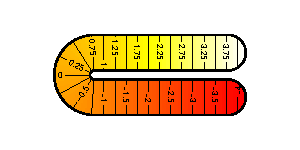
\includegraphics{intro/figs/orig-fs.pdf}\\
\caption{The horseshoe function as it appeared in \citeb{ramsay}.}
\label{orig-fs}
\end{figure}

As mentioned above, when the smoothing problem is specified in terms of Euclidean distance, the model takes the distance between the points in the two arms of the horseshoe as the distance over the gap in-between them, rather than the distance along the major axis of the shape. This causes the high function values from one side to contaminate the other side (and the low to contaminate the high).
		
\subsection{Previous approaches to leakage}
\label{intro-leakageapproaches}

The cause of leakage can be characterized in two ways: either the smooth does not respect the boundary of the domain, or the smooth does not take into account the geometry of the domain (in particular with regard to the distance between points within the domain). Previous work in this area has been to combat leakage along these two lines. Work of \citeb{ramsay} and \citeb{soap} both use a partial differential equation (PDE) boundary condition approach to try to prevent leakage, whereas \citeb{wangranalli} and \citeb{eilerstalk} modify the way that inter-point distances are measured in order to avoid smoothing across boundaries. These four main works are now summarized.

\begin{enumerate}
\item \citeb{ramsay} proposes finite element $L$-splines (FELSPLINEs). The $L$-spline penalty is similar to the one in (\ref{intro-2d-objfcn}):
\be
\int_\Gamma (L_p f)^2 \text{d}\mathbf{x}.
\ee
Integration is performed over $\Gamma$ (the domain over which the smoothing is to take place) and $L_p$ is a roughness operator defined as:
\be
L_p=\Delta^p+c_{p-1}\Delta^{p-1}+\dots+c_1\Delta+c_0I.
\ee
Here $I$ is the identity operator, the $(c_0,\dots, c_p)$ are constants and $\Delta$ is the Laplacian (sum of second derivatives with respect to $x_1$ and $x_2$). This can be thought of as simply replacing the $P$ operator in (\ref{intro-2d-objfcn}) and changing the integration domain. 

In order to find $f$ Ramsay takes a finite element approach. First triangulating the domain, then constructing a set of bivariate quadratic polynomial basis functions over each triangle, specifying that there be continuity over the edges of the triangles. By taking the FELSPLINE objective function and transforming it into a variational form (as one would for a PDE), the approximation to the minimizer of the objective function is found.

Since the triangulation and hence the penalty of the FELSPLINE is only calculated over the domain, and the continuity is specified over neighbouring cells, the method prevents leakage. However, although FELSPLINE does not exhibit leakage on the original horseshoe (\fig{orig-fs}), in practice the model makes unrealistic physical assumptions. The boundary conditions of FELSPLINE specify that the gradient is zero, along normals to the boundary. This is not always physically realistic. \citeb{soap} show that by modifying the test function on horseshoe domain (see \secref{sc-alt-horsehoe}), the FELSPLINE performance begins to falter.

FELSPLINE does not offer a realistic physical model and is therefore not a viable solution to the finite area smoothing problem in general.

\item \citeb{wangranalli} adopt a ``within-area distance'' formulation for thin plate splines. They choose to use the geodesic distance between two points, that being the shortest path within the domain. This gives a definition of how near objects are in the domain. The within-area distances are used in the radial basis functions in place of the Euclidean norm (\secref{GAMtprs}).

To calculate the distances, Wang and Ranalli first create a complete, weighted, undirected, graph ($G$, say) with a data point at each vertex and the distance between each pair of vertices as the weights on the edges. They then find the restricted graph of $G$, $G_k$, in which each vertex is only connected to its $k$ nearest neighbours. With this new, restricted graph the geodesic distances between each pair of vertices can be calculated using Floyd's algorithm (\cite{Floyd}).

As the authors point out, the quality of the approximation is dependent on the size of the data set and its density. At low densities the estimated geodesic distance will tend towards the Euclidean, at high densities the approximation tends, asymptotically toward the true geodesic distance (\cite{bernstein}). Even if  dense enough data were available, the method will be rather slow since Floyd's algorithm is cubic in the number of vertices (the size of the data set). 

Taking these points into account, Wang and Ranalli's approach appears cumbersome, slow and dependent on dense data.

\item The soap film smoother (\cite{soap}) uses a rather simple physical model to prevent leakage from occurring. First, consider the domain boundary to be made of wire, then dip this wire into a bucket of soapy water, you will then have a soap film in the shape of your boundary. Consider the wire to lie in the $x_1-x_2$ plane and the height of the soap film at a given point to be the functional value of the model (i.e. in the $z$ direction). This film is then distorted smoothly by moving it toward the data, while minimising the surface tension in the film.

Fitting a model using the soap film smoother consists of first finding a set of basis functions which are solutions to a series of partial differential equations (PDEs) which define the film. Since these functions arise from PDE with boundary conditions, the resulting functions respect those boundary conditions (which can be estimated from the data or set to some known values), by default. 

Although mathematically elegant, the soap film smoother is a rather complex and computationally expensive model (since the series of PDEs must be solved every time). One must also pick knots for the soap film smoother to use, introducing an element of arbitrariness into the fitting process. The model also treats the boundary as something special, it is not clear that this is always appropriate (in particular thinking of ocean-based studies where some of the boundaries are coastlines but others are essentially arbitrary).

Although not perfect, the soap film smoother will be used throughout the thesis a the ``gold standard'' against which the methods proposed herein will be measured. The soap film was chosen over the other methods above since it is already implemented in the \textsf{R} package \texttt{soap} (unlike GLTPS, which does not have an easily available implementation) and it does not have any obvious major technical flaw (like the unrealistic physical assumptions that FELSPLINE makes).

Chapter \ref{chap-it} gives the technical details relating to the construction of the basis. The chapter also further illustrates the soap film smoother via a case study showing its use as the spatial part of a spatiotemporal model for the incidence of resident foreigners in Italy. 

\item An alternative approach to treating the boundary as something special is to transform the space in which the points lie to a different domain which is more suitable for smoothing. For example, with Ramsay's horseshoe, it seems intuitive to simply bend the horseshoe into a long strip and then smooth on that domain.

\label{cor-3s2}Indeed, \citeb{eilerstalk} proposed using the \textit{\sch\ transform} for this very purpose (the author independently came to the idea in 2008). The basic idea is to find a function that takes points in the domain the data lie in and maps them to another domain in which smoothing is easier. Using the \sch\ transform for smoothing will be investigated in chapter \ref{chap-sc}.

Outside of the smoothing spline and GAM literature, transformation-based methods have also been suggested, in particular, when using a kriging approach (see \citeb[pp. 425-430]{MASS} for a concise introduction, \citeb{schabenberger} or \citeb{diggle} for a thorough treatment). Kriging consists of modelling the spatial correlation between points via the \textit{semivariogram} and a spatial trend via a mean function (similar to the linear predictor in the smoothing case, although there are flavours of kriging where the mean is considered constant and/or known). Semivariogram models assume that the correlation between points is related to the distance between the points but not their position (this is known as \textit{stationarity}, and comes in varying degrees, \citeb[pp. 42-44]{schabenberger}). When the boundary of the domain has a complex shape, the correlation between points is likely to vary with distance within the domain rather than the Euclidean distance between points. Simply substituting within-area distances into the semivariogram will lead to an invalid semivariogram (\secref{gds-krig}; \cite{curriero})

Several authors have suggested the use of some kind of transformation of the data points in space in order to maintain stationarity by approximating within-area distances with equivalent Euclidean distances via \textit{multidimensional scaling} (\cite{mdskrig}; \cite{crabkrig}; \cite{curriero}). The use of multidimensional scaling to project these distances ensures that the semivariogram remains positive or conditionally negative definite (which is required to have a valid semivariogram, \citeb{curriero}).

%Although not specifically designed to deal with leakage issues (although leakage manifests itself as a breakdown of stationarity in a kriging context), several authors have suggested the use of some kind of transformation of the data points in space in order to maintain stationarity by approximating within-area distances with equivalent Euclidean distances via \textit{multidimensional scaling} (\cite{mdskrig}; \cite{crabkrig}; \cite{curriero}). 

Using multidimensional scaling as a transformation of a spatial domain is investigated in chapters  \ref{chap-mds} and \ref{chap-gds}. A comparison between the geostatistical implementations and the methods developed in this thesis is given in \secref{gds-krig}, once the proposed methods have been fully explained.
\end{enumerate}

Creating some kind of mapping between the space in which the data lies and the space in which conventional smoothers perform well is convenient. Relying on existing, tested methodology is clearly appealing. Transformation-based approach also benefit from not treating the boundary as a special in the basis setup. The properties that such a mapping would require to be useful for smoothing will be investigated in subsequent chapters.

Chapters \ref{chap-sc}, \ref{chap-mds} and \ref{chap-gds} investigate the combination a transformation of space and conventional smoothers to solve the problem of leakage in finite area smoothing. The next chapter attempts to solidify the concepts presented so far (smoothing, penalties, leakage, tensor products) as well as highlight some of the potential pitfalls when modelling complex data. The chapter applies a spatiotemporal model of legal immigrants in Italy using a tensor product of a soap film smoother basis (for space) and a cubic spline basis (for time).

\chapter{The \sch\ transform as a method for finite area smoothing}
%\begin{quotation}
%``Failure is \textit{always} an option.'' 
%
%-- Adam Savage
%\end{quotation}

% schwartz-christoffel stuff

\label{chap-sc}

\section{Introduction}

This chapter investigates the efficacy of using a conformal mapping to transform the domain in which we wish to perform smoothing. The mapping takes points in the domain of the data ($W$) to a domain on which it is easier to smooth ($W^*$). In particular the utility of the \sch transform is examined (elaborating on \cite{eilerstalk}).

Given some region that it is difficult to smooth over, one approach is to transform the domain in which the problem resides. So, for example, one could transform a region into a rectangle, circle or other familiar shape to avoid the problems such as leakage. In this spirit, we wish to find some mapping such as $\phi$ in \fig{simpledia}.

This kind of approach is appealing since it allows the use of existing techniques in the transformed domain (\emph{ie.} not having to resort to model and basis reformulation). It also feels more natural to treat the domain as if it were made of silly putty and simply squash the region into the shape required to perform analysis.

% Simple diagram showing the mapping
\begin{figure} [htbp]
\centering
\includegraphics[scale=0.3]{sc/figs/simpledia.pdf}
\caption{An example of a transformation; the function $\phi$ takes the points in the rectangle and maps them to the region on the left.}
\label{simpledia}
\end{figure}

The \sch mapping offers such a transformation; it takes some arbitrary polygon and maps it to some specified shape. The most common domains to transform to are: (i) the upper half-plane ($H^+$), (ii) a rectangle and (iii) the unit disk. This is achieved in the $H^+$ case by taking the vertices of the polygon and mapping them to points on the real line (see \fig{reallinedia}). This can be thought of as ``unwrapping'' the polygon onto the real line. For the unit disk case, points on the circle bounding the unit disk map to vertices on the polygon (see \fig{unitdiskdia}). One can think of this as adding control points to the unit circle and then altering the angles. The rectangular case is somewhat similar to the unit disk in that extra points are added to the boundary and the angles of these points tightened until the shape is identical to the polygon. Obviously, those points lying inside the polygon are also moved around due to the mapping, creating a new (non-uniform) distribution of space.

% Diagram showing upper half plane to polygon
\begin{figure} [tbp]
\centering
\includegraphics[scale=0.6]{sc/figs/reallinedia.pdf}
\caption{A mapping of the upper half-plane to the polygon. The vertices ($w_k$) are the result of applying $\phi$ to the points on the real line ($w^*_k$). The boundary of the polygon is mapped to the real line. Note that the final vertex, $w^*_6$ is mapped to the point $\infty$ on the real line.}
\label{reallinedia}
\end{figure}

% Diagram showing unit disk to polygon
\begin{figure} [tbp]
\centering
\includegraphics[scale=0.6]{sc/figs/unitdiskdia.pdf}
\caption{A mapping of the upper half-plane to the polygon. The vertices ($w_k$) are the result of applying $\phi$ to the points on the real line ($w^*_k$). The boundary of the polygon is mapped to the boundary of the unit disk.}
\label{unitdiskdia}
\end{figure}

The goal is to transform the domain with the complex boundary, then smooth in the transformed domain. The procedure we wish to perform is as follows:

\begin{enumerate}
\item Determine the domain over which we would like to smooth, $W$. This could be the region or a bounding box around it.

\item Compute the \sch transform of $W$ to get $W^*$. Obtaining the function, $\phi$.

\item Map the co-ordinates of the datapoints in $W$ to $W^*$.

\item Fit the GAM to the data in $W^*$.

\item Perform any further inference (in $W$ or $W^*$, since there is a 1-1 mapping between them.)
\end{enumerate}

The second section of this chapter explains the technical details of the mapping. The third section gives results of some simulations and the final section summarises the results and draws conclusions from them.

\section{Technical details}

This section gives some of the mathematical and computational details required to calculate the \sch mapping. The primary reference is the extremely thorough work of \cite{driscoll}, which covers almost all aspects of the \sch transform.

\subsection{Nomenclature}

The polygon is first defined formally along with its associated quantities, as they will be referred to throughout the rest of the chapter.

A polygon, $\Gamma$, is a collection of vertices $w_1, w_2,\dots,w_n$ and interior angles $\alpha_1\pi, \alpha_2\pi, \dots, \alpha_n\pi$. For convenience we define $w_{n+1} = w_1$ and $w_0=w_n$. Numbering of vertices is anti-clockwise. The angles are such that $\alpha_k \in (0,2]$ and we require:
\begin{equation}
\sum_{k=1}^n (1-\alpha_k) = 2.
\end{equation}
The external angle, $\theta_k\pi$, as given by $(1-\alpha_k)\pi$ (see \fig{anglediagram}).

% Diagram showing the exterior/interior angle relationship.
\begin{figure} [bp]
\centering
\includegraphics[scale=0.6]{sc/figs/anglediagram.pdf}
\caption{The external angle $\theta_k$ is associated with the vertex $w_k$. The internal angle is given by $\alpha_k$. Shading indicates the inside of the polygon.}
\label{anglediagram}
\end{figure}

The boundary of the polygon is denoted by $\Gamma$. We refer to two domains: $W$ and $W^*$, denoting the original domain (inside $\Gamma$) and the transformed domain (of the plane, unit disk or rectangle) respectively. 

Vertices on the polygon are denoted as $w_k$ and those on the transformed boundary are denoted as $w^*_k$ (the \emph{prevertices}). In general a point in the polygon's original domain is denoted as $w$ and in the transformed domain as $w^*$.

We use the function $\phi$ to map from the transformed domain to the polygon (\emph{ie.} $\phi:W^* \mapsto W$). The inverse mapping function, $\phi^{-1}$, is used to go from the polygon to one of: the unit disk, rectangle or half-plane ($\phi:W \mapsto W^*$).  See \fig{mappingdia}.

% Mapping diagram from my whiteboard
\begin{figure} [tbp]
\centering
\includegraphics[scale=0.5]{sc/figs/mappingdia.pdf}
\caption{Diagram showing the forwards and backwards mappings with their relations to the mapped and unmapped spaces in the rectangular case.}
\label{mappingdia}
\end{figure}

\subsection{\sch Mapping}
\label{schparprob}
We now look at the mathematical formulation for the upper half-plane, unit disk and rectangle. There are many mappings that can be performed however those detailed here are either canonical (in the case of the half-plane) or considered to be useful in a smoothing context (the other two).

For the purposes of smoothing we are interested in the function $\phi^{-1}$ (\emph{ie.} the function that goes from our domain to the transformed one). We must first calculate $\phi$ before we may calculate its inverse. In the literature $\phi$ is referred to as the \emph{forwards map} and $\phi^{-1}$ as the \emph{backwards map}.

The forwards map, $\phi$, is determined up to translation, scaling, and rotation by the prevertices (see below). So, our task is to efficiently find the prevertices and hence find the mapping $\phi$. The task of obtaining the prevertices is known as the \emph{\sch parameter problem}.

\subsubsection{The upper half-plane}
\label{sc-parprob}

When mapping $\Gamma$ to $H^+$ we set $\phi(\infty) = w_n$ without any loss of generality. \cite{driscoll}, p. 10 then gives the following formula formula:
\begin{equation}
\phi(w^*) = A + C \int^{w^*}_{w^*_0} \prod_{k=1}^{n-1} (\zeta-w^*_k)^{\alpha_k-1} d\zeta.
\end{equation}
Here $A$ and $C$ are complex constants determined once the $w^*_k$ have been calculated. These control the scaling, translation, and rotation of the transform.

Although setting $\phi(\infty) = w_n$ does not make any difference in a mathematical sense, it does mean that the density of the points mapped into $H^+$ is rather odd. Given two adjacent points near $w_n$, their spacing on the upper half-plane is huge in comparison to two adjacent points near the other vertices. For this reason the $H^+$ mapping is not pursued further here.

\subsubsection{Unit disk}

The formula for the unit disk looks very similar to that for $H^+$ but the product now runs over all prevertices. The integrand is simply a constant multiple of the $H^+$ case. This is merely to avoid problems in the calculation of the branch cuts (\cite{driscoll}, p. 12).
\begin{equation}
\label{unitscmap}
\phi(w^*) = A + C \int^{w^*}_{w^*_0} \prod_{k=1}^{n} (1 - \frac{\zeta}{w^*_k})^{\alpha_k-1} d\zeta.
\end{equation}
As above, $A$ and $C$ are complex constants responsible for scaling, translation, and rotation.

\subsubsection{Rectangle}
For the rectangle case we must specify four vertices of $\Gamma$ that map to the four corners of the rectangle. This uniquely specifies the aspect ratio of the rectangle (\cite{driscoll}, p. 48).

The rectangle mapping is slightly different in its calculation to the two above mappings. We first map $\Gamma$ to the upper half-plane as detailed above. From there we can use the Jacobi elliptic function (\cite{handbuch} p. 701):
\be
F(\gamma,k)=\int_0^\gamma \frac{dt}{\sqrt{1-k^2\sin^2t}}
\ee
to map a rectangle to the upper half-plane. The computation of this map is expensive due to the evaluation of the elliptic function (\cite{driscoll}, \emph{p. 49}) so a shortcut is used by mapping to the strip. We do not go into further about detail here (as the computational intricacies are covered in \cite{howell90}).

\subsection{Computation of the \sch mapping}

To compute the map, we need to find the prevertices, $w^*_k$; since the complex constants just control scaling, translation, and rotation, we can compute them after computing the $w^*_k$. We achieve this iteratively by approximating the $w^*_k$ then mapping those points back to the polygon to give an estimate to $\Gamma$, $\Gamma^\prime$. 

To measure the quality of approximation of $\Gamma^\prime$ to $\Gamma$ we use the following set of equations:
\begin{equation}
\label{optimizeme}
\frac{\vert \phiinv(w_{k+1}) -  \phiinv(w_k) \vert}{\vert \phiinv(w_2)-\phiinv(w_1)\vert} - \frac{\vert w^*_{k+1} - w^*_k\vert}{\vert w^*_2 - w^*_1\vert} = 0, \qquad \text{for } k=3,\dots,n-1.
\end{equation}
Here $\vert \phiinv(w_{k+1}) -  \phiinv(w_k) \vert$ is the distance between the $k^{\text{th}}$ and $(k+1)^{\text{th}}$ vertex.  We find this by integrating along the line between the points within $W$.

Intuitively, we are comparing the side lengths of the polygon in order to evaluate approximation of $\Gamma$ in each iteration (\cite{snider}, A-3). Both of these measures are scaled by the distance between the first two vertices (in their respective domains).

Note that \eqn{optimizeme} does not include the vertex $w_n$. By theorem 3.1 of \cite{driscoll}, p. 24) a polygon is precisely defined by its angles and its vertices not including $w_n$ (since if we know the direction of the edges leaving $w_1$ and $w_{n-1}$, we may find the point where they meet). It is for this reason, in the upper half-plane case, that we can map $w_n$ to $\infty$ without loss of generality.

Also note that \eqn{optimizeme} does not include $w_1$ or $w_2$ in the numerator on the right hand side. This is due to all vertices (and hence $w_1$ and $w_2$) being rescaled, rotated, and translated by the complex constants, $A$ and $C$, in the \sch formula.

In practice we fix $w^*_n=1$, $w^*_{n-1}=-i$ and $w^*_{n-2}=-1$ in the unit disk case (\cite{driscoll}, p. 24.) For the rectangle case we need to specify which vertices of $\Gamma$ will map to which vertices of the rectangle.

The scaling factor, $C$, (from \eqn{unitscmap}) may be calculated using:
\begin{equation}
C=\frac{\vert \phiinv(w_2)-\phiinv(w_1)\vert}{\vert w_2 - w_1\vert}.
\end{equation}
Otherwise, we can assume that up to scaling and rotation that $w_1$ and $w_2$ are correct. In which case we know that $\Gamma$ and $\Gamma^\prime$ are similar (in the geometric sense). 

$A$ is the image of the base point of the integration and is usually written as $w_0$. For computational reasons this is usually the prevertex nearest to the point $w^*$ that we wish to map in \eqn{unitscmap}  (\cite{driscoll}, \emph{p. 27}).


\subsubsection{Sketch of an algorithm to calculate the \sch mapping}
\label{algorithmsketch}
\begin{enumerate}
\item Accept inputs:
   \begin{enumerate} 
      \item $w_1,\dots,w_n$ (the vertices),
      \item $n$ (the number of vertices),
      \item $\alpha_1,\dots,\alpha_n$ (the internal angles at each vertex).
   \end{enumerate}
\item Define the objective function, $F$, as:
 \begin{equation*}
F=\frac{\vert \phiinv(w_{k+1}) -  \phiinv(w_k) \vert}{\vert \phiinv(w_2)-\phiinv(w_1)\vert} - \frac{\vert w^*_{k+1} - w^*_k\vert}{\vert w^*_2 - w^*_1\vert}, \qquad \text{for } k=3,\dots,n-1,
 \end{equation*}
\item Use steepest descent and then Newton's method to until $\vert F\vert < \epsilon \quad \forall k$. \item Calculate $C$ and $A$ as detailed above.
\item Return values for $w^*_1,\dots,w^*_n$, $C$ and $A$.
\end{enumerate}

Starting values for the algorithm are evenly spaced vertices around the edge of the disk/rectangle or, in the case of the plane, along the real line. Not including those vertices specified as being fixed, above.

\subsection{Getting between $W$ and $W^*$}

\subsubsection{Forwards map}

Calculating the forwards map is simply a case of evaluating $\phi$ at the necessary points. If we wish to find the point on polygon ($w$), given some known point on the disk ($w^*$), we compute:
\begin{equation}
\label{forwardsmap}
w=\phi(w^*) = w_0 + C \int_{w^*_0}^{w^*} \prod_{k=1}^{n} (1 - \frac{\zeta}{w^*_k})^{-\theta_k} d\zeta,
\end{equation}
where $w^*_0$ is any point in the closed disk such that $w_0 = \phi(w^*_0)$ is known and non-infinite. We may choose any point since the integrand is analytic throughout the mapping and hence the integral is path-independent (\cite{driscoll} \emph{p. 27}). A common choice for $w_0$ is the centre of the polygon.

Equivalent expressions exist for the rectangle and upper half-plane cases (see \cite{driscoll} p. 49 and p. 10, respectively).

\subsubsection{Backwards map}

To calculate the backwards mapping, there are two possible approaches: (i) using Newton's method to solve the equation $\phi(w^*)-w=0$ and (ii) solving the initial value problem (IVP):
\begin{equation}
\label{scivp}
\frac{dw^*}{dw}=\frac{1}{\phi^{-1}(w^*)} \quad \text{and} \quad \phiinv(w_0)=w^*_0.
\end{equation}
In fact a combination of these methods are used. Solving \eqn{scivp} approximately gives the starting values for the Newton iterations which are significantly faster (since $\phi^{-1}$ is cheaper than $\phi$ to compute.) (\cite{driscoll} \emph{p. 29}).

The only problem with this is that the path from $w_0$ to the point to map, $w$, must lie entirely inside the polygon. Whether this is true is not known, since after the mapping has been computed, the only known points are the vertices (at which the IVP is singular). So, to combat this, all points on the path are checked sequentially. This computation, although inelegant, is fast compared to the IVP/Newton iterations.

An example of using the backwards map to find the transformed co-ordinates from a square to the unit disk is given in \fig{squaredomain}. An irregular nonagon is given in \fig{irregdomain}.


% Square domain mapping diagram
\begin{figure} [bp]
\centering
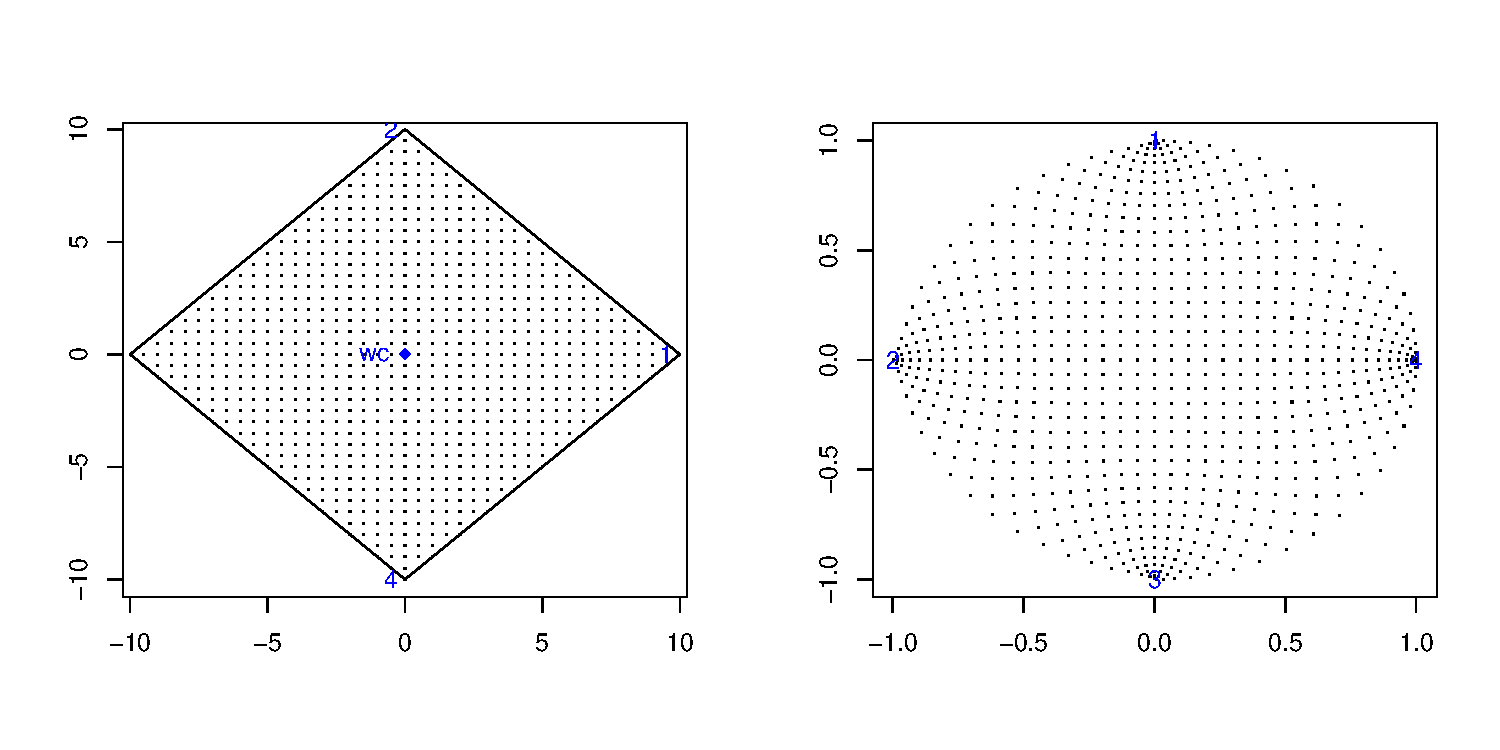
\includegraphics[scale=0.5]{sc/figs/squaredomain.pdf}
\caption{A regular grid of points over the square region (left). The right panel shows the mapping of these points under the \sch transformation to the unit disk.}
\label{squaredomain}
\end{figure}

% Irregular mapping diagram
\begin{figure} [tbp]
\centering
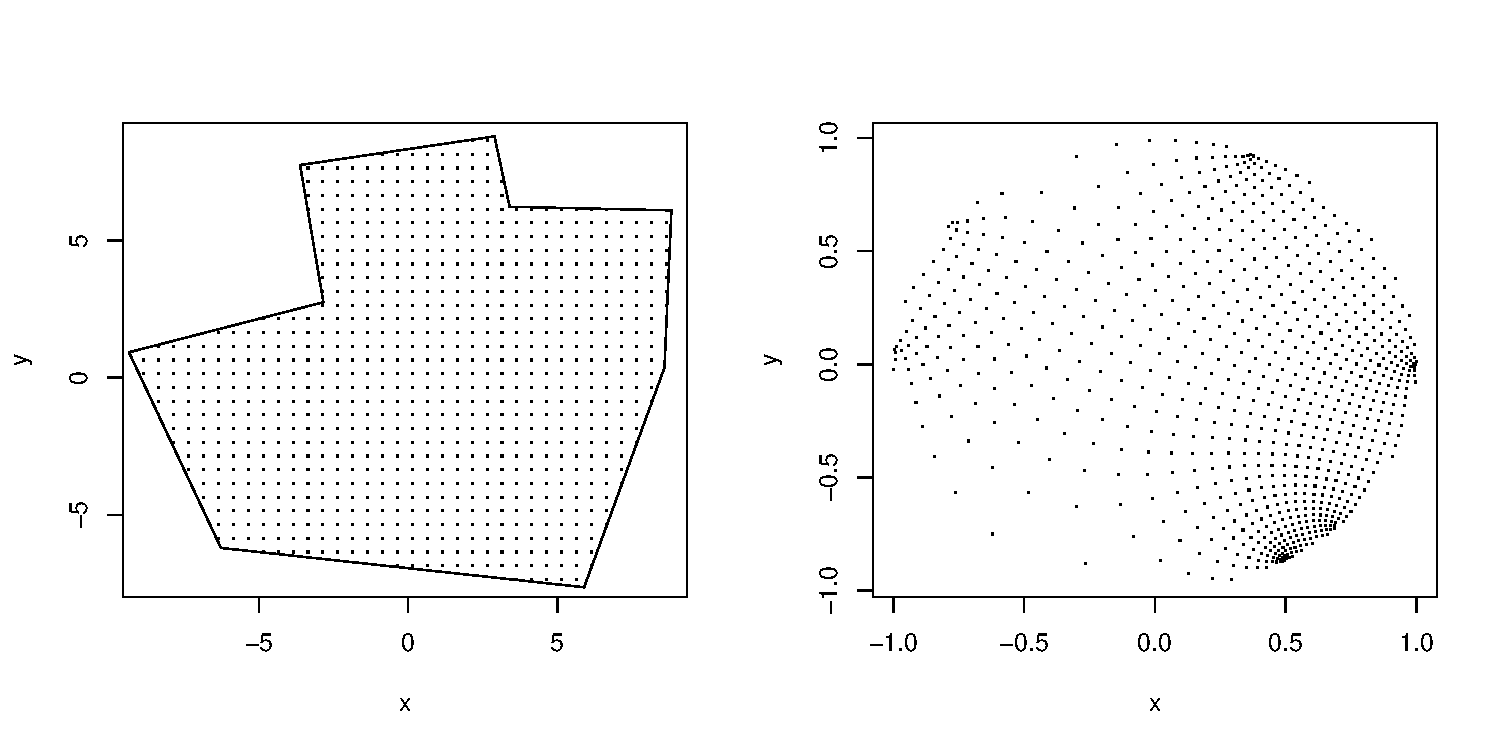
\includegraphics[scale=0.5]{sc/figs/irregulardomain.pdf}
\caption{A regular grid of points over region bound by a irregular nonagon (left). The right panel shows the mapping of these points under the \sch tranformation to the unit disk.}
\label{irregdomain}
\end{figure}

\subsection{Crowding}

\subsubsection{The crowding problem}
When the polygon is elongated or has many vertices, the mapped vertices may be positioned too closely in the transformed domain. This effect is referred to as \emph{crowding} and can be observed in \fig{crowdeddisk}. In elongated regions prevertices can be located exponentially close such that they are indistinguishable in finite precision arithmetic (\cite{howell90}).

% Crowded mapping diagram
\begin{figure} [tbp]
\centering
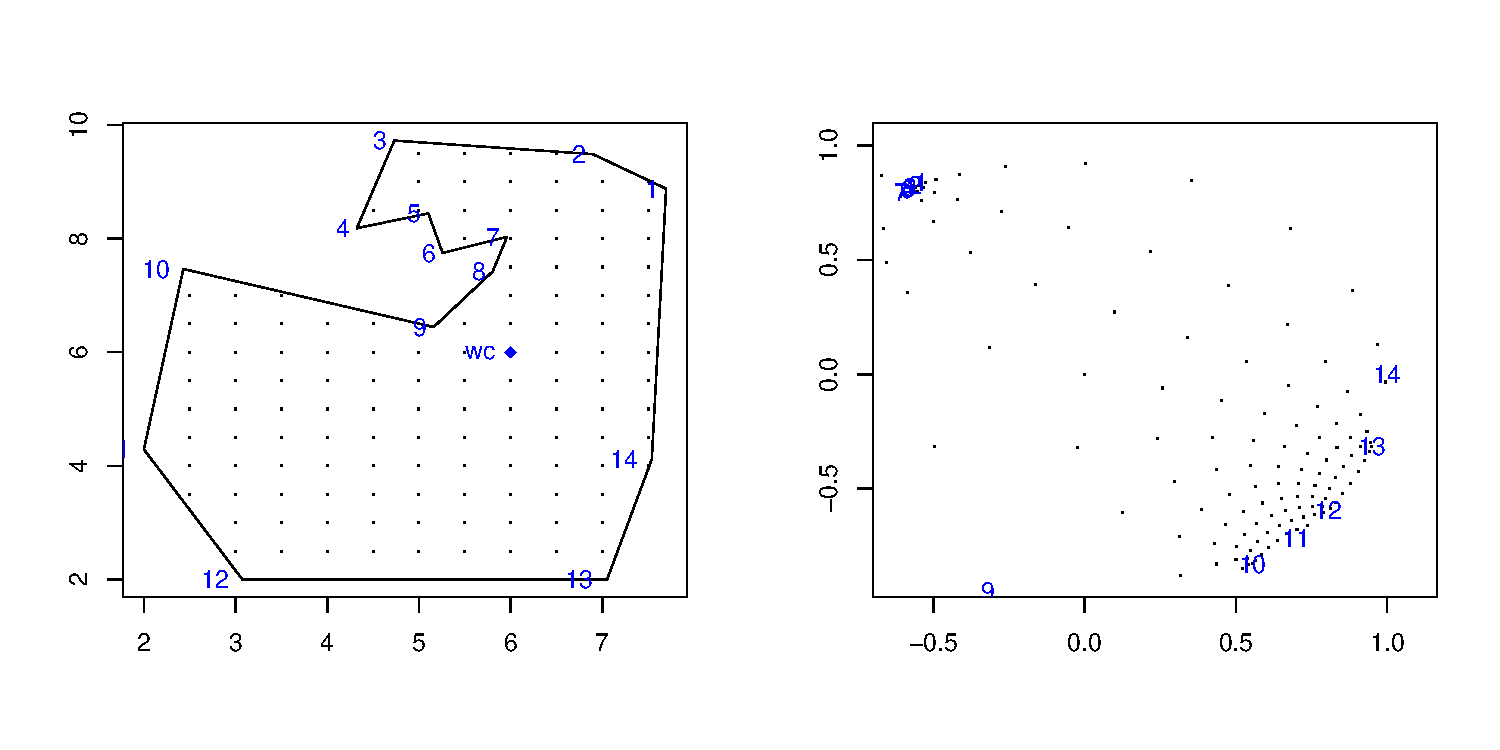
\includegraphics[scale=0.5]{sc/figs/crowdeddisk.pdf}
\caption{An example of crowding. Note that prevertices 1 through 8 are mapped almost to a singularity in the right panel.}
\label{crowdeddisk}
\end{figure}

\subsubsection{Fixing crowding}

If the crowding is caused by $\Gamma$ being elongated then a  primitive fix is to map to an elongated domain such as the rectangle or plane. This approach is suggested in \cite{howell90} however, as they point out, this does not eliminate all crowding and problems can still occur when there are strongly acute peninsulae in the polygon. Mapping to an elongated domain also does not fix problems which occur when mapping from T- or H-shaped domains (so-called ``multiply elongated'' domains.)

In order to combat this problem more effectively, \cite{vavasis96} propose the CRDT (cross-ratios of the Delaunay triangulation) algorithm (see below). Each set of prevertices has $n-3$ degrees of freedom hence, there is a three parameter family of possible vertex arrangements that all map to the same polygon. The most stable of these \emph{embeddings} should be used. The M\"{o}bius transformation relates the embeddings to one another.

This idea can be extended by noting that the polygon is identical when additional vertices are added between the current ones, provided that the internal angle associated with the new vertex is $\pi$. These extra vertices also do not change the \sch formula since in \eqn{unitscmap} $\alpha_k=1$ for an angle of $\pi$. Adding these extra vertices allows us to control the aspect ratio of the mapping.

In the solution to the \sch parameter problem given in \secref{sc-parprob}, conditions on the side lengths and orientations of the polygon are enforced. The CRDT algorithm imposes conditions about quadrilateral sections of the polygon and the diagonals of the polygon. First a Delaunay triangulation of the domain is performed and then pairs of triangles are merged into quadrilaterals. A measure is then defined (the \emph{cross-ratio}) which specifies a set of non-linear equations to be solved. These equations enforce the constraint that the cross-ratio in mapped polygon comes out correctly. 

Putting all of these ideas together gives the CRDT algorithm. We first add edges to the polygon with internal angle $\pi$ to remove enlongated parts of the domain and then triangulate the domain. Once the domain is triangulated we calculate the cross-ratio:
\begin{equation}
\rho(a,b,c,d) = \frac{(d-a)(b-c)}{(c-d)(a-b)},
\end{equation}
for each quadrilateral in the polygon. Then, analogously to \eqn{optimizeme} we set up a series of equations, specifying that the cross-ratios remain the same in the polygon and the transform of the rectangle back to the polygon. We then wish to solve for the values of $\rho$ for the original domain in the same manner as we solved for side lengths in the original problem. 

In \fig{uncrowdeddisk} the CRDT method is used with a rectangular domain, crowding has been alleviated to some degree. The point density, as well as vertex density seems to be more uniform than in \fig{crowdeddisk}.

% Uncrowded mapping diagram
\begin{figure} [tbp]
\centering
\includegraphics[scale=0.5]{sc/figs/irregular-fixed-crdt.pdf}
\caption{The mapping of the irregular domain featured in \fig{crowdeddisk} using the CRDT method mapping to a rectangle. The crowding is now much less severe.}
\label{uncrowdeddisk}
\end{figure}

The downside of using CRDT is that it may add too many vertices to maintain the aspect ratio (\cite{driscoll05}), so the algorithm tends to take longer than the one specified in \secref{algorithmsketch} since it is $O(n^3)$ JUSTIFY AND ELABORATE ON THIS!. This is, of course, offset against the fact that the problem becomes tractable.






\section{Simulation experiments}

In order to test the efficacy of the \sch transform for the purposes of smoothing over complex regions, a series of simulation experiments were performed. The \emph{SC Toolbox} for MATLAB was used to perform the transform and the mapping of the points. These were then fed into \textsf{R} and models run using packages \texttt{mgcv} and \texttt{soap}.

\subsection{Ramsay horseshoe}

The most obvious candidate for simulation is the Ramsay horseshoe (see \secref{ramsayfunc}). In order to map the horseshoe, we first draw a rough bounding box around the shape. In order to map as simple a domain as possible, to begin with a bounding box was used as the $W$ domain remapped via the \texttt{evalinv()} function from the \emph{SC Toolbox}. This is shown in \fig{hswithboundingbox}. The bounding box is then transformed to the rectangle. 

\begin{figure}
\centering
% trim order l b r t
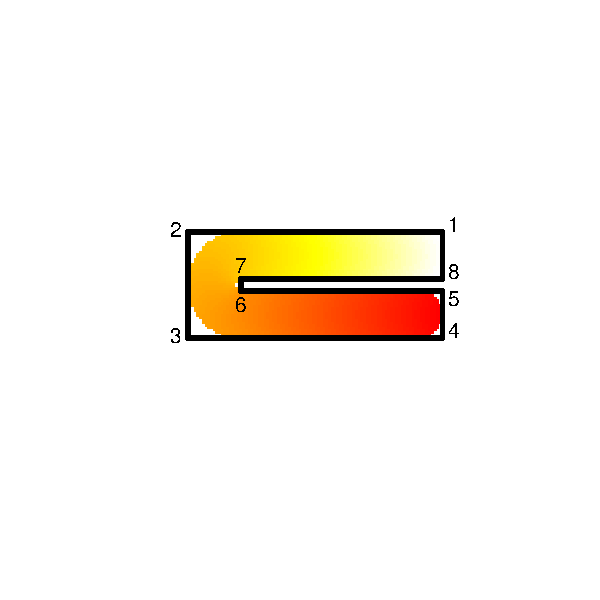
\includegraphics[trim=0.5in 1in 0in 0.5in]{sc/figs/hswithboundingbox.pdf} \\
\caption{The horseshoe with its bounding box. The vertices marked 1, 4, 5 and 8 are mapped to the corners of the rectangle.}
\label{hswithboundingbox}
% generated by /phd-smoothing/sc-writeup/figs/hswithboundingbox.R
\end{figure}

A sample of 1000 points was then taken from the horseshoe and noise added to the data. First the $x$,$y$ coordinates of the sampled points were expressed as complex numbers of the form $w=x+iy$. The sample was then mapped into $W^*$, creating a new set of coordinates $w^*=x^*+iy^*$. Smoothing was then performed over the responses in the $W^*$ domain using the \texttt{gam()} function in \texttt{mgcv}. 

\begin{figure}
\centering
% trim order l b r t
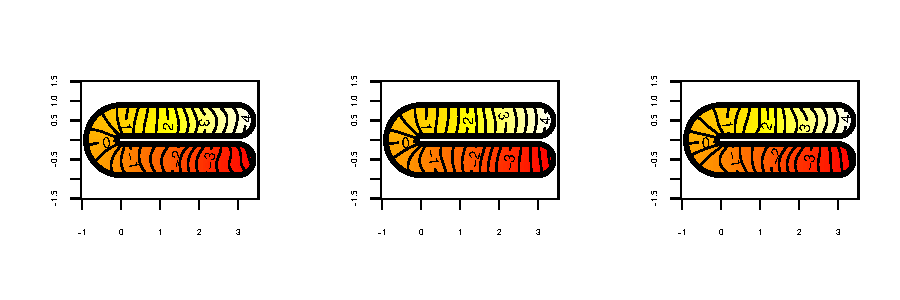
\includegraphics[width=4in]{sc/figs/compsmooth.pdf} \\
\caption{Comparison of smooths given using P-splines on the transformed domain (top right), thin plate splines on the transformed domain (bottom left) and soap film smoother (bottom right) for the Ramsay horseshoe (top left). Here sample size was 250, noise level was set to $\sigma=1$.}
\label{compsmooth}
% generated by figs/pspline.soap.comp.hs.R
\end{figure}

\Fig{compsmooth} shows the true function and typical realisations of: the fit given using a \tprs without transformation, the fit given by a \tprs with transformation and the fit given by the soap film smoother. Looking at the heat maps one can see that the horseshoe function is clearly However, visual inspection alone is clearly not enough basis for accepting the method, therefore we now look at the mean squared error of the models.

Note that using the SC transform, we don't capture the curvature in the function.


\begin{table}[tb]
\begin{tabular}{c c}\\
$n$ & $\sigma$ \\
\hline
\hline
1000 & 0.3 \\
500 & 0.3 \\
250 & 0.3 \\
100 & 0.3 \\
1000 & 0.5 \\
1000 & 1 \\
1000 & 2 \\
\end{tabular}
\caption{Setup for the simulations using the \sch transform for the Ramsay horseshoe. Sample size is $n$ and $\sigma$ is the number a random deviate from a standard Normal distribution was multiplied by before being added to the true test function.}
\label{scramsimtable}
\end{table}

\Tabref{scramsimtable} shows the settings for noise level and sample size of the simulations. Mean squared error between the true function and the fitted model was used to evaluate the model's performance. In the following tables we provide the mean squared error over a prediction grid of 1000 points averaged over 1000 generated data sets.

\Tabref{scramsayres} shows the results from the simulations for the standard horseshoe. A cursory glance show that that results were better than those for the soap film smoother for larger sample sizes and standard errors were comparable. Once we get to 100 samples the method performance degrades over all methods. Once noise is introduced into the data we can see that the soap film and transformation method do as well as each other, MSEs are approximately the same and the standard errors are of the same order.

SAY SOMETHING ABOUT THE BOXPLOTS. THEY NEED TO BE REGENERATED!!!!

\begin{figure}
\centering
% trim order l b r t
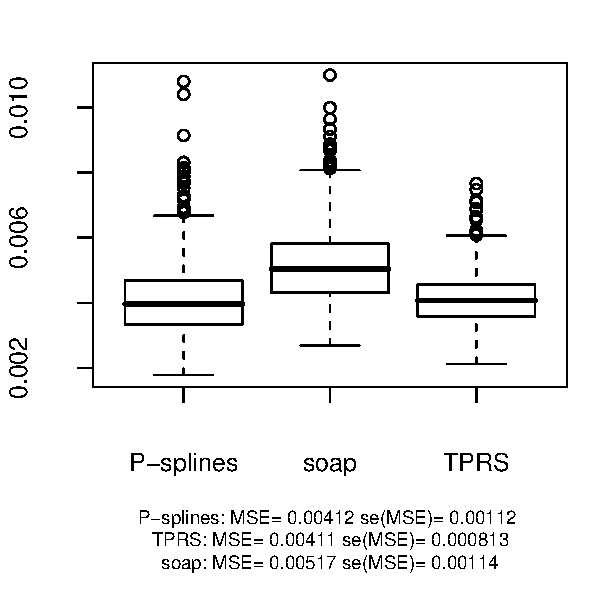
\includegraphics{sc/figs/mses-boxplot.pdf} \\
\caption{Boxplots of mean MSE from 1000 points on a prediction grid from 1000 simulations.}
\label{scram1000boxplots}
% generated by ramsaysim/makeboxplots.R
\end{figure}

\begin{table}[ht]
\begin{tabular}{c c c c c}\\
Sample size & Noise level & P-spline MSE (\emph{sd}) & Thin plate MSE (\emph{sd}) & Soap MSE (\emph{sd}) \\
\hline
\hline
1000 & 0.3 & 0.00412 (0.00112) & 0.00811 (0.00243) & 0.00517 (0.00114) \\ 
500 & 0.3 & 0.00505 (0.00144) & 0.00478 (0.000955) & 0.00628 (0.00146) \\ 
250 & 0.3 & 0.00875 (0.00392) & 0.00684 (0.00183) & 0.0107 (0.00305) \\ 
100 & 0.3 & 0.0225 (0.035) & 0.0118 (0.00461) & 0.0219 (0.0117) \\ 
1000 & 0.5 & 0.0105 (0.00353) & 0.00811 (0.00243) & 0.0127 (0.0034) \\ 
1000 & 1 & 0.0242 (0.0108) & 0.0161 (0.0069) & 0.0275 (0.00958) \\ 
1000 & 2 & 0.066 (0.0481) & 0.0388 (0.0229) & 0.0686 (0.0333) \\ 
\end{tabular}
\label{scramsayres}
\caption{Mean squared error along with its standard deviation for the transformed Ramsay horseshoe (for P-spline and thin plate cases) versus those for the soap film smoother.}
% generated by /phd-smoothing/sc-writeup/tablecode/ramsay.sim.results.table.R
\end{table}


NEED TO ADD A BIT MORE HERE

Need to re-run some of the simulations so that they have the right models. From there adjust the tables and boxplots accordingly. Then re-write the brief analysis bit here!




Looking at the predicted values for the model in the $W^*$ domain we get an indication as to why the fit is so good. \Fig{hsvisgam} shows predictions from the fitted surface alongside the true values when the domain has been put into its ``natural'' coordinate system. The coordinate system for the fitted values is the \sch transformed system and for the true values the system is the major and minor axes of the shape (\emph{ie.} one axis along the central curve of the shape and the other perpendicular to that.) In the plot, the strong linear trend along the major axis of the horseshoe can be seen in both cases, making this a rather trivial smoothing problem. So, it looks like the problem is being addressed in a close approximation to its natural domain.

\begin{figure}
\centering
% trim order l b r t
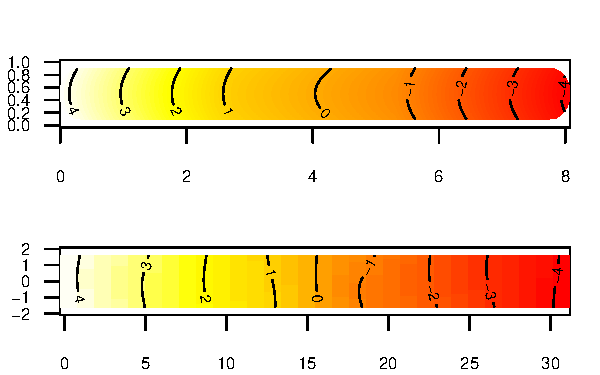
\includegraphics[trim=0in 0.5in 0in 0in]{sc/figs/hsvisgam.pdf} \\
\caption{Heatmap of the true values of the modified Ramsay horseshoe projected into it's natural domain (left) and the predicted values of the fit given using the \sch transform and then smoothed using a \tprs (right.)}
\label{hsvisgam}
% generated by /phd-smoothing/thesis/sc/figs/hsvisgam.R
\end{figure}

\subsubsection{Alternate Ramsay horseshoe}

The second domain tested was the alternate version of the Ramsay horseshoe from \cite{soap}. For this domain the gradient runs across the short axis of the horseshoe. A heatmap of this test function can be seen in \fig{altramsayhorseshoe}. The same simulation setup was used as for the first domain and can be seen in \tabref{scramsimtable}.

\begin{figure}
\centering
% trim order l b r t

\includegraphics[trim=0.5in 1in 0in 0.5in]{sc/figs/altramsayhorseshoe.pdf} \\
\caption{Heatmap of the alternate version of the Ramsay horseshoe.}
\label{altramsayhorseshoe}
\end{figure}


NEED TO RE-RUN THESE ANALYSES TOO! ALSO reanalyse them!



For the alternative horseshoe we begin to see the soap film creep ahead of the transformation method (see \tabref{scaltramsayresultstable}.) Although the MSEs are of approximately the same order (as are the standard errors), the soap film is gaining ground. 




To examine what is going on here we can look at the plots of the predicted values as heat maps. These can be seen in \fig{altramsaycomp} and show that the \sch mapping seems to capture the overall structure of the shape better than the soap film smoother, which seems to capture patches of the shape but not the overall structure. It also appears that the \sch method does not respect the ends of the horseshoe and continues the gradient running along the minor axis over this part as well.This feature seems to be the cause of the performance decrease.

------------------------


\begin{table}[ht]
\begin{tabular}{c c c c c}\\
Sample size & Noise level & P-spline MSE (\emph{sd}) & Thin plate MSE (\emph{sd}) & Soap MSE (\emph{sd}) \\
\hline
\hline
1000 & 0.3 & 0.00415 (0.00117) & 0.0158 (0.00247) & 0.00378 (0.00108) \\ 
500 & 0.3 & 0.00469 (0.00147) & 0.00793 (0.00186) & 0.00458 (0.00145) \\ 
250 & 0.3 & 0.00716 (0.00431) & 0.0142 (0.00249) & 0.00771 (0.00301) \\ 
100 & 0.3 & 0.039 (0.22) & 0.0201 (0.00589) & 0.0298 (0.42) \\ 
1000 & 0.5 & 0.00839 (0.00403) & 0.0158 (0.00247) & 0.00966 (0.00371) \\ 
1000 & 1 & 0.0194 (0.0122) & 0.0226 (0.0085) & 0.019 (0.00981) \\ 
1000 & 2 & 0.0605 (0.0468) & 0.0436 (0.0276) & 0.041 (0.0434) \\ 
\end{tabular}
\label{scaltramsayresultstable}
\caption{Mean squared error along with its standard deviation for the transformed alternate Ramsay horseshoe (for P-spline and thin plate cases) versus those for the soap film smoother.}
% generated by /phd-smoothing/sc-writeup/tablecode/alt.ramsay.sim.results.table.R
\end{table}

\begin{figure}
\centering
% trim order l b r t
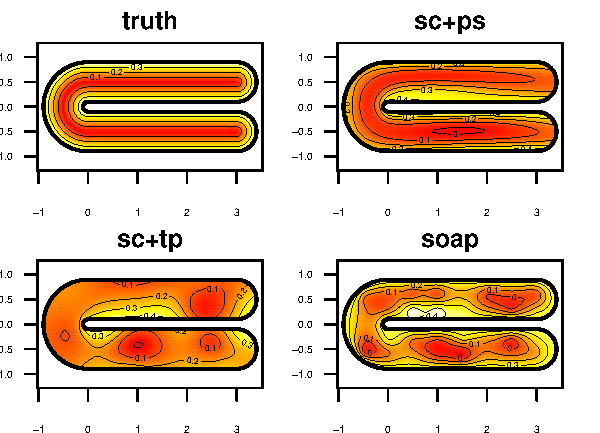
\includegraphics[width=4in]{sc/figs/altramsaycomp.pdf}\\
\caption{Single realisations of the fit to the alternate Ramsay horseshoe for each method. Clockwise from top left: the original figure, the function estimated by the \sch transform with P-splines, function estimated by the \sch transform with thin plate splines and finally the soap film estimate. Error set to $\sigma=1$.}
\label{altramsaycomp}
% generated by /phd-smoothing/sc-writeup/figs/altramsaycompare.R 
\end{figure}


\subsubsection{What's happening?}

At this point it is useful to get an idea about what the transformation is doing to the domain, specifically to find out about the distortion to space caused by the transform. To investigate this we can take a straight line in the $W$ domain and see what it maps to in the $W^*$ domain. We can also look at the response along that line according to the transformed and untransformed coordinate systems and see how this compares to looking at the response in the horseshoe's natural coordinate system.

\begin{figure}
\centering
% trim order l b r t

\includegraphics[trim=0.5in 1in 0in 1in]{sc/figs/horseshoecentreline.pdf} \\
\caption{Mapping of a straight line along the major axis of the Ramsay horseshoe to its position in the ``unwrapped'' domain.}
\label{horseshoecentreline}
% generated by /phd-smoothing/ramseysim/nullspace.test.R 
\end{figure}

\Fig{horseshoecentreline} shows the line that was evaluated along the centre of the horseshoe and its equivalent line in the transformed domain. We can see from this that a line that is straight in the domain appears to be bent in the transform. The curvature does not appear to be particularly extreme in this case, however, one can imagine that this could get significantly worse for regions with more complicated boundaries. Although this is interesting, it is more revealing to look at the evaluations of the horseshoe functions along that line.

\Fig{centrelinelineplot} shows the evaluations of the horseshoe function over the line plotted against three coordinate systems. The first plot shows the function evaluations on the $W$ domain as a response to change in $y$. The second on the $W^*$ domain, as a response to $y^*$, in the transformed coordinate system. The final plot is in the horseshoe's ``natural'' domain, \emph{ie.} the value the horseshoe takes as a function of distance along the major axis of the shape. From these plots one can see the quality of approximation to the natural domain of the horseshoe the \sch transform affords. Only two minor kinks occur in the line. Looking at where the kinks occur, they correspond exactly to those kinks in \fig{horseshoecentreline}. This makes sense, since we would expect a change in gradient if direction we are traveling has moved into two dimensions from one.

\begin{figure}
\centering
% trim order l b r t
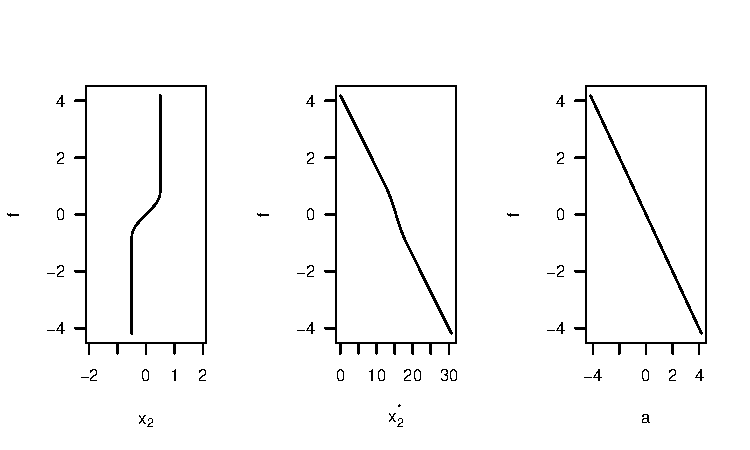
\includegraphics[trim=0in 0in 0in 0in]{sc/figs/centrelinelineplots.pdf} \\
\caption{Plots of the horseshoe function against the $y$ axis for (left) the untransformed horseshoe, (middle) the shape under the \sch transform and, (right) the function evaluation against the major axis.}
\label{centrelinelineplot}
% generated by /phd-smoothing/ramseysim/nullspace.test.R 
\end{figure}


\Fig{altcentrelinelineplot} shows analogous plots to \fig{centrelinelineplot} and backs up this hypothesis. The second panel shows the mapping of the $y$ component of the centreline against the response and the third panel shows the same in the horseshoe's own domain. The two plots appear to be indistinguishable.

\begin{figure}
\centering
% trim order l b r t
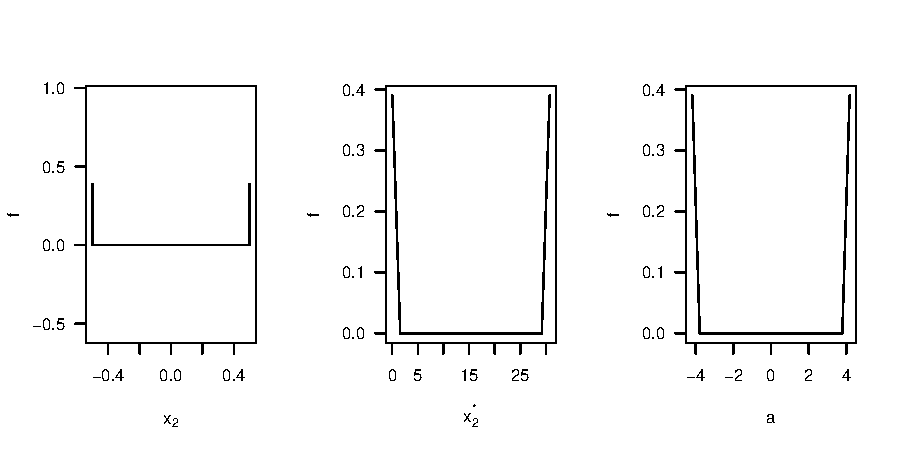
\includegraphics[trim=0in 0in 0in 0in]{sc/figs/altcentrelinelineplots.pdf} \\
\caption{Plots of the alternate horseshoe function against the $y$ axis for (left) the untransformed horseshoe, (middle) the shape under the \sch transform and, (right) the function evaluation against the major axis.}
\label{altcentrelinelineplot}
% generated by /phd-smoothing/altramsaysim/nullspace.test.R 
\end{figure}



\section{Conclusions \& Analysis}





Why this doesn't work but why it wasn't a waste of time.


\chapter{Multidimensional scaling for domain-dependent finite area smoothing}

% Writeup for MDS
% David Lawrence Miller
% d.l.miller@bath.ac.uk
  
\documentclass[a4paper,10pt]{article}
\setlength{\textheight}{22.5cm}
\setlength{\textwidth}{6.47in}
\setlength{\oddsidemargin}{-1mm}
\setlength{\topmargin}{0.1cm}
\setlength{\evensidemargin}{-5mm} 
 
% Load some packages
\usepackage{times, amsmath, amssymb, amsfonts, url, natbib, bm, rotating}
 
\usepackage{multirow}
\usepackage{graphicx}
\usepackage{rotating}
\usepackage{psfrag}

% top matter
\title{Multidimensional scaling as a tool for \\smoothing over complex regions}
\author{David Lawrence Miller\\Mathematical Sciences\\University of Bath\\\texttt{d.l.miller@bath.ac.uk}}
 
% Shortcuts
% Probability
\newcommand{\prob}[1]{\mathbb{P}\left[ #1 \right]}
% Schwarz-Christoffel
\newcommand{\sch}{Schwarz-Christoffel }
% fprime
\newcommand{\fprime}{f^\prime(z)}
% figure reference command
\newcommand{\fig}[1]{\emph{fig.} \ref{#1}}
% Figure reference command
\newcommand{\Fig}[1]{\emph{Fig.} \ref{#1}}
% table reference command
\newcommand{\tabref}[1]{\emph{table} \ref{#1}}
% Table reference command
\newcommand{\Tabref}[1]{\emph{Table} \ref{#1}}
% equation reference command
\newcommand{\eqn}[1]{(\ref{#1})}
% phi inverse
\newcommand{\phiinv}{\phi^{-1}}
% use other phi
\renewcommand{\phi}{\varphi}
%transpose
\newcommand{\tr}[1]{#1^{\text{T}}}
% diagonal
\newcommand{\diag}{\text{diag}}
% call \times \cross
\newcommand{\cross}{\times}


\begin{document}
 
% The abstract
%\begin{abstract}
%Here.
%\end{abstract}
 
 
% New theorem for theorems
\newtheorem{thm}{Theorem}[section]
 
%New theorem for definitions
\newtheorem{defn}{Definition}[section]
 
\maketitle

\section{Introduction}

\subsection{Motivation}

Splines are a popular way of performing spatial smoothing in two dimensions. In this context, they are used to fit smooth functions over a geographical region. A typical application of this is in ecological modelling; particularly when the spatial distribution of a species is sought. In this case counts of the species in question at the locations at which they were observed are recorded and fed into the model which can then be used to perform inference on the population, whether that be an abundance estimate, density map or a more sophisticated inferential goal.

When the geographical region has a complex boundary, features from one part of the domain can unduly influence other parts. Typically a ``complex boundary'' consists of having some peninsula-like feature(s) in the domain with notably different values on either side of the feature; there must also be some scientific motivation as to why those parts of the domain should not affect each other. Features such as peninsulae give rise to a phenomenon known as leakage; a typical example can be seen in \fig{leakage}. Leakage is problematic since it causes the fitted surface to be mis-estimated; this can then lead to incorrect inference (eg. incorrect abundance estimates), which is clearly not desirable. This can be seen in \fig{leakage} where the high values in the upper part of the domain leak across the gap to the lower values below and vice versa.

The cause of leakage can be thought of in two ways: either the smooth does not respect the boundary of the domain, or the smooth does not take into account the internal geometry of the domain; in particular with regard to the distance between points in the domain. Previous work in this area has been to combat leakage along these two lines. Work of \cite{ramsay} and \cite{soap} both use a PDE boundary condition approach to try to prevent leakage, where as \cite{wangranalli} attempt to approximate the within-area distances. In this report I will be adopting the the latter approach.

% leakage example 
\begin{figure}
\centering
% trim order l b r t
\includegraphics[width=4in]{figs/ramsay-leak.pdf}\\
\caption{An example of leakage. A thin plate regression spline was fit to data sampled from the function on the left, here the model smooths across the gap in the middle of the domain (right.)}
\label{leakage}
\end{figure}


\subsection{Proposition}

Multidimensional scaling (MDS) or, as it is often referred to, principle coordinates (PCO) (\cite{gower1966}) is a method commonly used in multivariate analysis. It is closely related to techniques such as PCA (\cite{chatfieldcollins}, p. 200) and canonical correspondence analysis (\cite{terbraak}.) The starting point for MDS is a matrix of distances, representing some kind of dissimilarity between observations. This distance could be calculated from the data, for example ideological distance between politicians measured using NOMINATE scores (\cite{quantss}, p. 225), or could instead be distances that occur in the data naturally,  for example comparative distances between stimuli response in a psychological experiment (\cite{torgerson}.) Here we concentrate on geographical distances.

MDS takes this matrix of distances and projects the data in such a way that Euclidean inter-point distances in the projection are approximately the same as the distances in the matrix (\cite{chatfieldcollins}, p. 187.) If the matrix of distances is of rank $m$ then a projection in $m-1$ or less can be output, although a projection into 2 dimensions is a typical choice. For this reason one can also think of MDS as a dimension reduction technique, finding a projection of a data cloud into lower dimensional space, while still retaining information about the distances between the points.

When MDS is performed on some categorised set of dissimilarities (as is often the case in social science and psychology) it is referred to as non-metric MDS, where as on a continuous scale it is known as metric MDS, though they have different names, the calculations are identical (aside from the method of finding the distances.) Discussion here will focus on metric MDS.

Multidimensional scaling offers a framework for the problem of smoothing over a region with a complex boundary. Given the set of distances between the points in the domain, we can project those points into a configuration such that the distances between those points are approximately preserved. Now, if the Euclidean metric were to be used to calculate the distances between the points then the result from the projection would be identical to the starting point configuration (provided that we projected back into the same number of dimensions.) However, if it were possible to use a metric that took into account the distance within the boundary (a within-area distance) then the resulting configuration of points would (approximately) respect the boundary of the domain.

This approach can be justified in the following way. In many applications within-area distances is meaningful, given (as stated above) that there is some reasoning behind why certain parts of the domain should not affect one another. When within-area distances are meaningful, it makes sense to work with the structure of the domain rather than the somewhat arbitrary choice of Euclidean geometry. However, as literature on smoothing is firmly based in a Euclidean context, it would be preferable to perform the smoothing in Euclidean space. In this case the approximation to Euclidean space afforded by an MDS projection of the within-area distances offers a bridge between these two requirements.

\subsection{Procedure}

The proposed procedure is as follows: Given a sample $\{x_i, z_i : i=1\dots n\}$: the set of points in the domain over which smoothing is to be performed, $x_i$ is the location (a $k$-vector, although here 2-vectors are assumed throughout) of the $i^\text{th}$ point with response $z_i$. Here it is assumed that finding an MDS configuration of a set of points includes calculating the within-area distances between the points and then the distance matrix, as well as actually performing the MDS calculation.

\begin{enumerate}
\item Obtain the MDS configuration for the domain using some representative set of points over the area in question. The only use of the MDS locations obtained in this step is to define the configuration, they are discarded afterward. Representative points could be a grid over the domain or subset of $\{x_i : i=1\dots n\}$; more detail and justification is provided in section \ref{grids}, below.

\item Using the MDS configuration obtained above along with Gower's interpolation (see section \ref{gowers}) obtain the location of the sample in the MDS configuration: $\{\tilde{x}_i, z_i : i=1\dots n\}$.

\item Smooth $\{\tilde{x}_i, z_i : i=1\dots n\}$ using a regression spline.

\item To predict at a location $x_j$ in the original domain, use Gower's interpolation to 
obtain the point's location in the MDS space: $\tilde{x}_j$. Predict $\hat{z}_j$ using the smooth at $\tilde{x}_j$: this is the prediction at $x_j$.
\end{enumerate}

The rest of this report is structured as follows: in section 2 an overview of MDS is given, along with technical details of how the MDS configuration is calculated; section 3 focuses on how the within-area distances are found; section 4 shows some examples of this method on simulated data. I conclude with a proposed course of action to improve the method.

\section{Multidimensional Scaling}

The basic concept behind MDS is to take the data, calculate their within-area inter-point distances and then find a new coordinate system based on those inter-point distances. We do this by simply performing an eigen-decomposition on the (centred) matrix of distances between points. First a description of the MDS procedure when Euclidean distances are used is given, followed by the justification for the use of the same procedure when using within-area distances.

\subsection{Finding the new point configuration}

We first define $d_{ij}$ as the distance between the points $i$ and $j$. These are used to form a (symmetric) matrix, $D$, with $ij^{\text{th}}$ element $d^2_{ij}$. For the moment let us assume that $D$ is known and $d_{ij}$ Euclidean distance between points $i$ and $j$. 

\cite{diaconis08} gives a clear definition of the algorithm (due to \cite{schoenberg35} and \cite{torgerson}) for finding the new locations of points, which is outlined below. Further detail is given in \cite{principlesofMA}, pp. 104-108 and \cite{chatfieldcollins}, pp. 189-200.

First, suppose that the $n$ the unknown locations (in $n$ dimensions) in our MDS configuration are entries in an $n \times n$ matrix, $\tilde{X}^*$. Now let $S=\tilde{X}^{*} \tilde{X}^{*\text{T}} $, so $S$ is a matrix of scalar products of the point vectors, \emph{ie.} the $(i,j)^\text{th}$ element of $S$ is:
\begin{equation}
s_{ij} = x_i\tr{x_j},
\label{selem}
\end{equation}
$S$ is an $(n\cross n)$ matrix. Note that we may only find $\tilde{X}^*$ up to a translation and rotation, so it is assumed that the values in $\tilde{X}^*$ have been centred about the origin.

We now wish to relate $D$ to $S$. First, note that that $(i,j)^\text{th}$ element of D is 
\begin{equation}
d_{ij}^2 = (x_i-x_j)\tr{(x_i-x_j)} = x_i\tr{x_i} + x_j\tr{x_j}  -2 x_i\tr{x_j}.
\label{dij}
\end{equation}
Using \eqn{selem}, we can re-write \eqn{dij} as
\begin{equation}
D=\mathbf{s}_\text{diag}\tr{\mathbf{1}} + \mathbf{1}\tr{\mathbf{s}_\text{diag}} -2S.
\label{dijmat}
\end{equation}
where $\mathbf{1}$ is an $n \cross 1$ vector of 1s and $s_\text{diag}$ is the $n \cross 1$ vector of diagonal elements of $S$.

Defining:
\begin{equation}
H = I-\frac{1}{n}\mathbf{1}\tr{\mathbf{1}},
\end{equation}
where $I$ is the identity matrix, as usual, and $\mathbf{1}$ is an $n \cross 1$ vector of 1s such that $\mathbf{1}\tr{\mathbf{1}}$ is an $n \cross n$ matrix of 1s.

By pre- and post-multiplying any matrix by $H$ the matrix is double centred (such that row and column means are 0.) This is true since, pre- and post-multiplying \eqn{dijmat} by $H$ yields:
\begin{equation}
HDH = -2HSH.
\label{eqH}
\end{equation}
The first two terms in on the right hand side of \eqn{dijmat} going to zero since the rows of $\mathbf{s}_\text{diag}\tr{\mathbf{1}}$ and the columns of  $\mathbf{1}\tr{\mathbf{s}_\text{diag}}$ are constant. Since $S$ is already centred, $HSH=S$, so the following relation between $S$ and $D$ holds:
\begin{equation}
S = -\frac{1}{2}HDH.
\label{eqH}
\end{equation}

Now we can deal with $S$ rather than $D$. We must factor $S$ find $\tilde{X}^{*}$. One option to factor $S$ is to use the Cholesky decomposition, however, with MDS we are looking to decompose the space based on the directions of largest variation, \emph{ie.} those that have the largest contribution to $s_{ij}$. For that reason we use the eigen-decomposition.

Performing an eigen-decomposition n $S$, we obtain $S=U\Lambda\tr{U}$. Here $U$ is the $n \cross n$ orthogonal matrix of eigenvectors and $\Lambda$ is the $n \cross n$ diagonal matrix of eigenvalues, we may then obtain $\tilde{X}^*$ as:
\begin{equation}
\tilde{X}^*=U\Lambda^{\frac{1}{2}}.
\end{equation}

Following these steps $\tilde{X}^*$ is an $n \cross n$ matrix. The aim here is to smooth in two dimensions (and in general we would preform MDS and want to see a reduction in dimensionality) so, the directions with the two largest eigenvalues are chosen to represent the space since they contain the two largest sources in variation in distance (since they are the two largest contributions to $S$.) This gives the two dimensional representation of the data. So, defining $\tilde{X}$ to be the $n \cross 2$ dimensional matrix obtained from truncating the full new coordinate set to the first two columns in decreasing eigenvalue order, a lower dimensional representation has been obtained. More generally, we can reduce the $\tilde{X}^*$ to an $n \cross k$ matrix, where $k$ is the number of dimensions for the MDS representation of the data.

So, in order to obtain the MDS configuration of points (given that we have some set of inter-point distances) we merely need to double centre the matrix of distances and perform an eigen-decomposition on the resulting matrix, $S$. 

In our case, we would like $d_{ij}$ to be the shortest distance between the points, given the path between the points remains within the domain. Finding $d_{ij}$ is discussed in the next section, however it is first important to justify the use of these steps when non-Euclidean distances are used. 

One can think of the justification in the following way: given that the distances in $D$ obey the triangle inequality, all of the points in $D$ ($n$ of them if $D$ is $n \cross n$) may be represented in $n$ dimensional Euclidean space (at worst.) Hence, in the case where the $d_{ij}$ are Euclidean distances in two dimensions, the smallest dimensional space in which they can be represented is 2, but they may still reside in $n$-dimensional space with no loss of information about the distances. So, in the case when the distances in $D$ are shortest within-area distances, one can just think of the points in $D$ as residing in a higher number of dimensions in such a way that the distances between them are Euclidean.

Note that an additive constant can be computed and added to the non-diagonal entries of $D$ to ensure that the eigenvalues of $S$ are non-negative. However, this does not occur in any of the examples shown here.

Multidimensional scaling may be performed in \textsf{R} using the \texttt{cmdscale} function. 

\subsection{Gower's interpolation} 
\label{gowers}
It is likely that we may be in a position where the coordinate system has been found by MDS but we need to insert further points into our MDS representation for example when further data is collected, or in order to predict over points not in $\tilde{X}$. In this case we would like to insert those new points into the configuration given by MDS. A number of methods have been developed over the past 40 years; Gower's interpolation (\cite{gower1968}) is covered here.

Say we have some point, $x_{\text{new}}$ and we wish to find its new location, $\tilde{x}_{\text{new}}$ in the MDS configuration, $\tilde{X}$. The position of $\tilde{x}_{\text{new}}$ is at a distance from the points in $\tilde{X}$ which is approximately the same as that of $x_{\text{new}}$ to the points in the non-transformed space. 

Note that here we are assuming that a 2 dimensional projection has been used in the initial MDS configuration, obviously Gower's interpolation remains valid for the case in which the initial MDS projection is in $k$ dimensions.

\subsubsection{Gower's interpolation formula}

We may find the new position, $\tilde{x}_{\text{new}}$ , of some new datum $x_{\text{new}}$ using:
\begin{equation}
\tilde{x}_{\text{new}} = \frac{1}{2} \Lambda^{-1} \tr{\tilde{X}} \mathbb{D}.
\label{gower}
\end{equation}
Here $\Lambda$ ($2 \cross 2$) and $\tr{\tilde{X}}$ ($2 \cross n$) are as above, $\mathbb{D}$ ($n \cross 1$) is the centred distance from the points in the original configuration to the new point.

In Gower's paper, he defines the $i^\text{th}$ element of $\mathbb{D}$ as $-(d^2_{i,\text{new}}-\text{diag}(\tilde{X}^* \tilde{X}^{*\text{T}})_{ii})$, with $d^2_{i,\text{new}}$ being the squared distance from the $i^\text{th}$ point to the new point. The centring is given by the diagonal elements of $\tilde{X}^*\tilde{X^{* \text{T}}}$ \emph{ie}. the squared distances from the original points to the centroid of the MDS configuration. To avoid confusion (and to emphasise that the full $\tilde{X}^*$ matrix is used, rather than its truncated version), it may be easier to think of the expression for the $i^\text{th}$ element of $\mathbf{d}$ as $-(d^2_{i,n+1}-\text{diag}(S)_{ii})$. Using this expression in computation is more logical since $S$ is already known.

Gower's interpolation extends simply to the case when $m$ new points are inserted by thinking of $\tilde{x}_{\text{new}}$ as $k \cross m$ matrix and $\mathbf{d}$ an $n \cross m$ matrix.


\subsection{Practical considerations}

Gower's paper shows that performing MDS on a dataset is equivalent to performing MDS on a reduced set of points and then inserting the remaining points when the Euclidean metric is used to calculate the distances between the points. Extensive testing on a number of different domains has shown this to be true.

Before performing any analysis we must test that the method will be reliable and that the mapping that MDS produces is smooth (in terms of the spatial coordinates that it produces.) I first motivate the need for using a grid as a start point for the MDS configuration, and then show that the mapping produces smooth lines when within-area distances are used.

\subsubsection{Using grids as a starting point}
\label{grids}
Given that both the finding of the MDS configuration of the points and Gower's insertion rely on the eigenvalues of the original MDS configuration, obtaining representative eigenvalues is important. If those points used to create the initial MDS configuration are not representative of the whole domain, the eigenvalues and eigenvectors may fail to represent the space correctly and, as such, we may then insert the point(s) incorrectly. This could happen if the initial MDS configuration is created using only points from one half of the domain or, more pathologically, there were some trend in the locations, in this case only a portion of the full information about the domain would be included in the model. This would lead to the unrepresentative eigenvalues being calculated. Indeed, Gower points this out at the end of his 1968 paper.

When Euclidean distances are used to calculate $D$ the eigenvalues are found correctly given that there is one more point than there are dimensions in the space (\cite{landmark},) provided that the points are not collinear. However, it is not clear what a similar criteria would be for the shortest paths used here. 

A simple example of this problem is show in \fig{tshape}. Here, a regular grid has been generated inside a ``T'' shape (top left panel.) The point configuration found by using the full set of points is given in the top right panel. In the pathological case when either only the ``head'' or ``tail'' of the T are sampled and used to generate the MDS and the other half inserted (bottom left for head (red) inserted from tail (black), bottom right of tail (red) inserted from head (black)), one can see that those points inserted into the configuration become warped. 

% showing the the grid is necessary using the T shape
\begin{figure}
\centering
% trim order l b r t
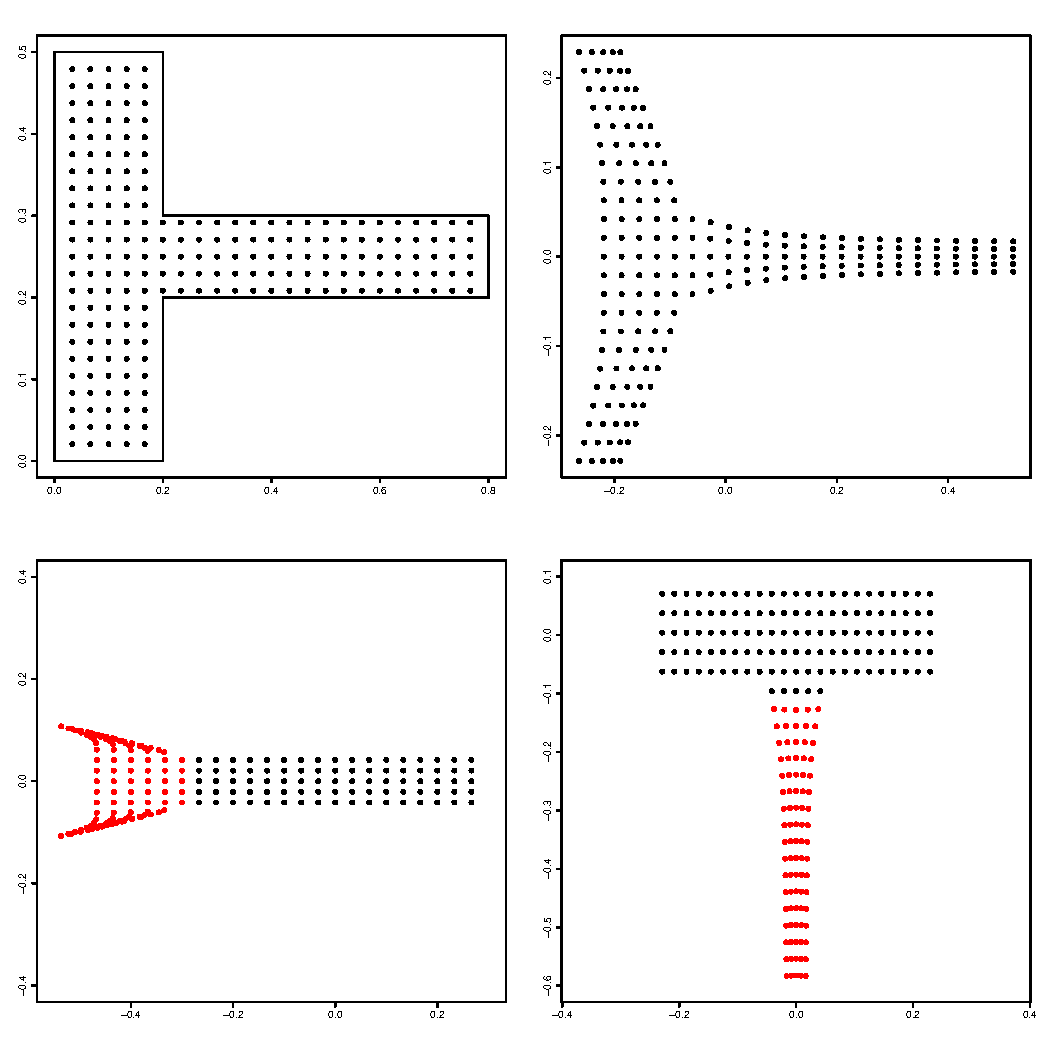
\includegraphics[width=3.5in]{figs/tshape.pdf} \\
\caption{Data generated inside a ``T'' shape (top left) is fed into MDS at once (top right.) When either the head or tail of the T is used for the original MDS configuration and the other points inserted, the shape produced is distorted.}
\label{tshape}
% generated using figs/gridtest.R
\end{figure}

Although the cases show in \fig{tshape} are somewhat pathological, looking at more reasonable situations still leads to wildly different results. In \fig{tshaperand} the black and green points make up the original MDS configuration; the five green points are chosen at random. The red points are then inserted. As can be seen in these four realisations, the shape of the MDS space is dependent on those points used to create the initial MDS configuration.

% showing the the grid is necessary using the T shape (random samples
\begin{figure}
\centering
% trim order l b r t
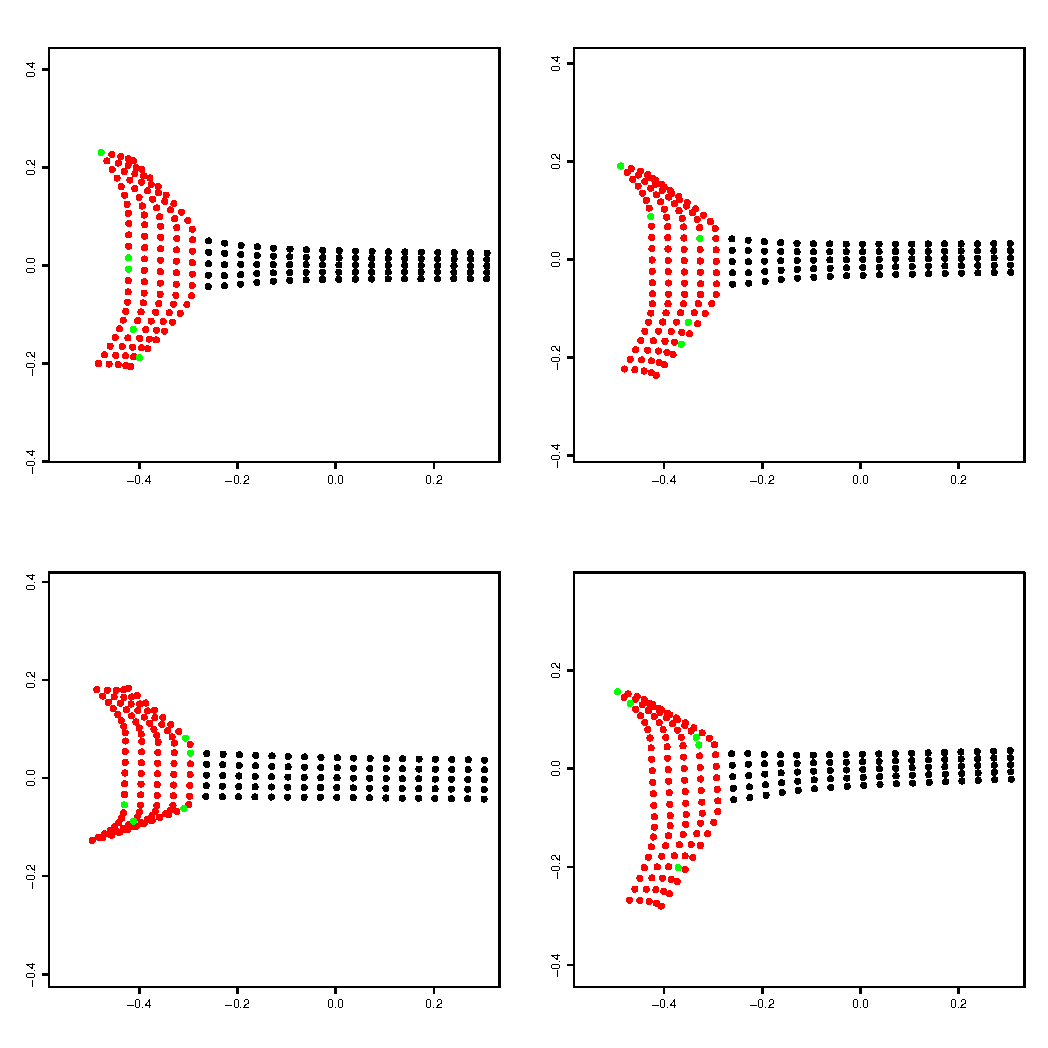
\includegraphics[width=3.5in]{figs/tshaperand.pdf} \\
\caption{Using the ``T'' shape in \fig{tshape}, the tail (black points) of the T was used with 5 randomly sampled (green) points in the head. The ``head'' (without the 5 green points) was then inserted into the MDS configuration (red.) As can be seen from these four realisations, the output varies greatly depending on the points sampled.}
\label{tshaperand}
% generated using figs/gridtest.R
\end{figure}

Hence, although there are the usual problems with predicting outside of one's dataset, the added problem of the instability of MDS insertion can only confound results further. (Again, this is mentioned at the end of Gower's paper.)

This problem can be rectified by using an appropriately spaced grid on the domain to calculate the eigen-decomposition, thus ensuring that the whole area is covered. The base MDS configuration is then stable, provided that the grid is fine enough to catch all the features in the boundary of the domain.

\subsubsection{Smoothness of mapping}

Following from this, it is important to make sure that the MDS space is smooth in the sense that a grid of smooth lines over the domain is mapped to a series of smooth lines without discontinuities or sudden changes in direction. Taking the evenly spaced grid in \fig{wt2-grid-orig}, first MDS is performed on a dense point set of size 1253, and then a less dense grid is inserted using the method of Gower. The grid produced under the insertion can be seen in \fig{wt2-grid-full}. Taking a sample of 250 points from the 1253, an MDS configuration was also found and the same grid inserted (see \fig{wt2-grid-samp}.) From this it is clear that those points mapped into the domain are smooth but in the sample case the features in the far right of the shape (the less pronounced peninsulae) are squashed down.

% grid to map
\begin{figure}
\centering
% trim order l b r t
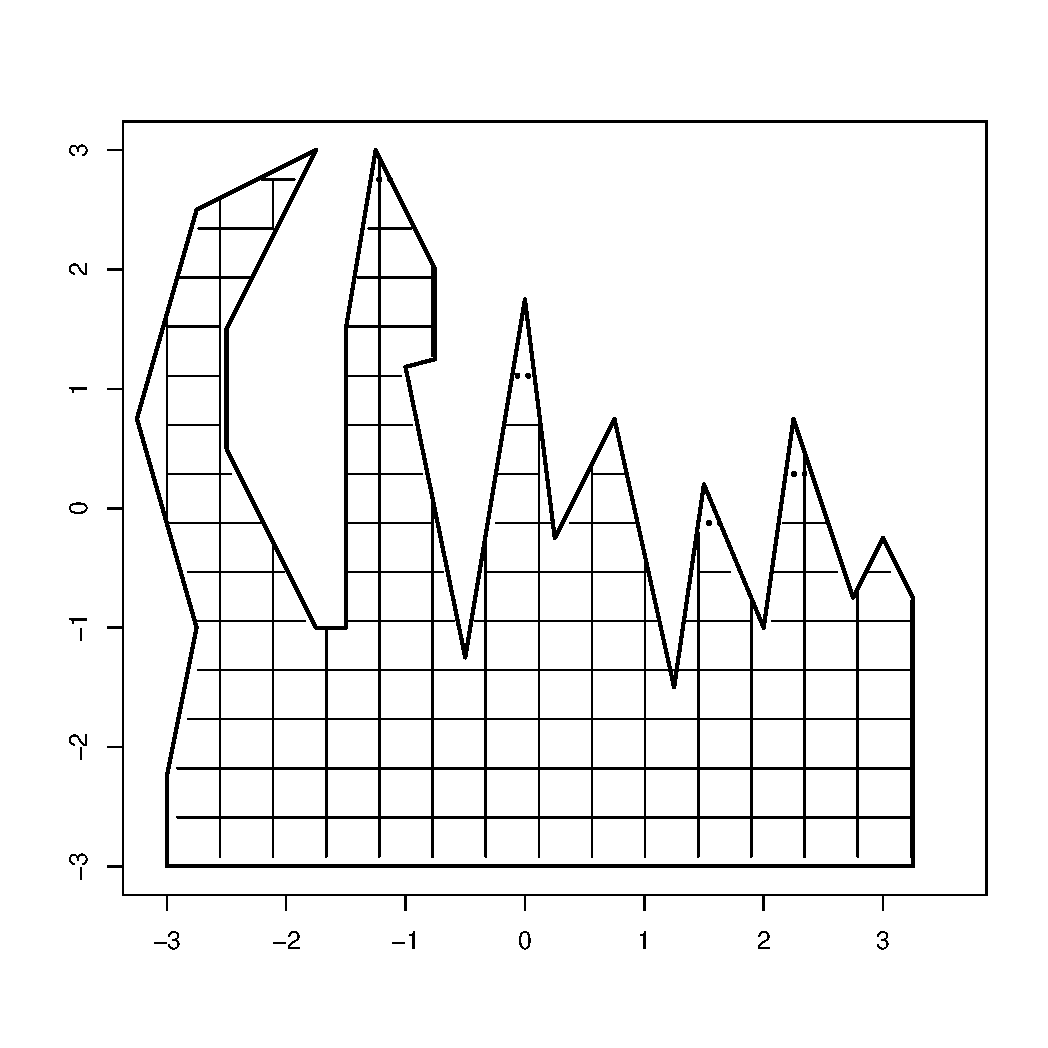
\includegraphics[width=4in]{figs/wt2-grid-orig.pdf} \\
\caption{The grid to be inserted into the MDS configuration.}
\label{wt2-grid-orig}
% generated using wt2-grid.R
\end{figure}

% mapped grid (full)
\begin{figure}
\centering
% trim order l b r t
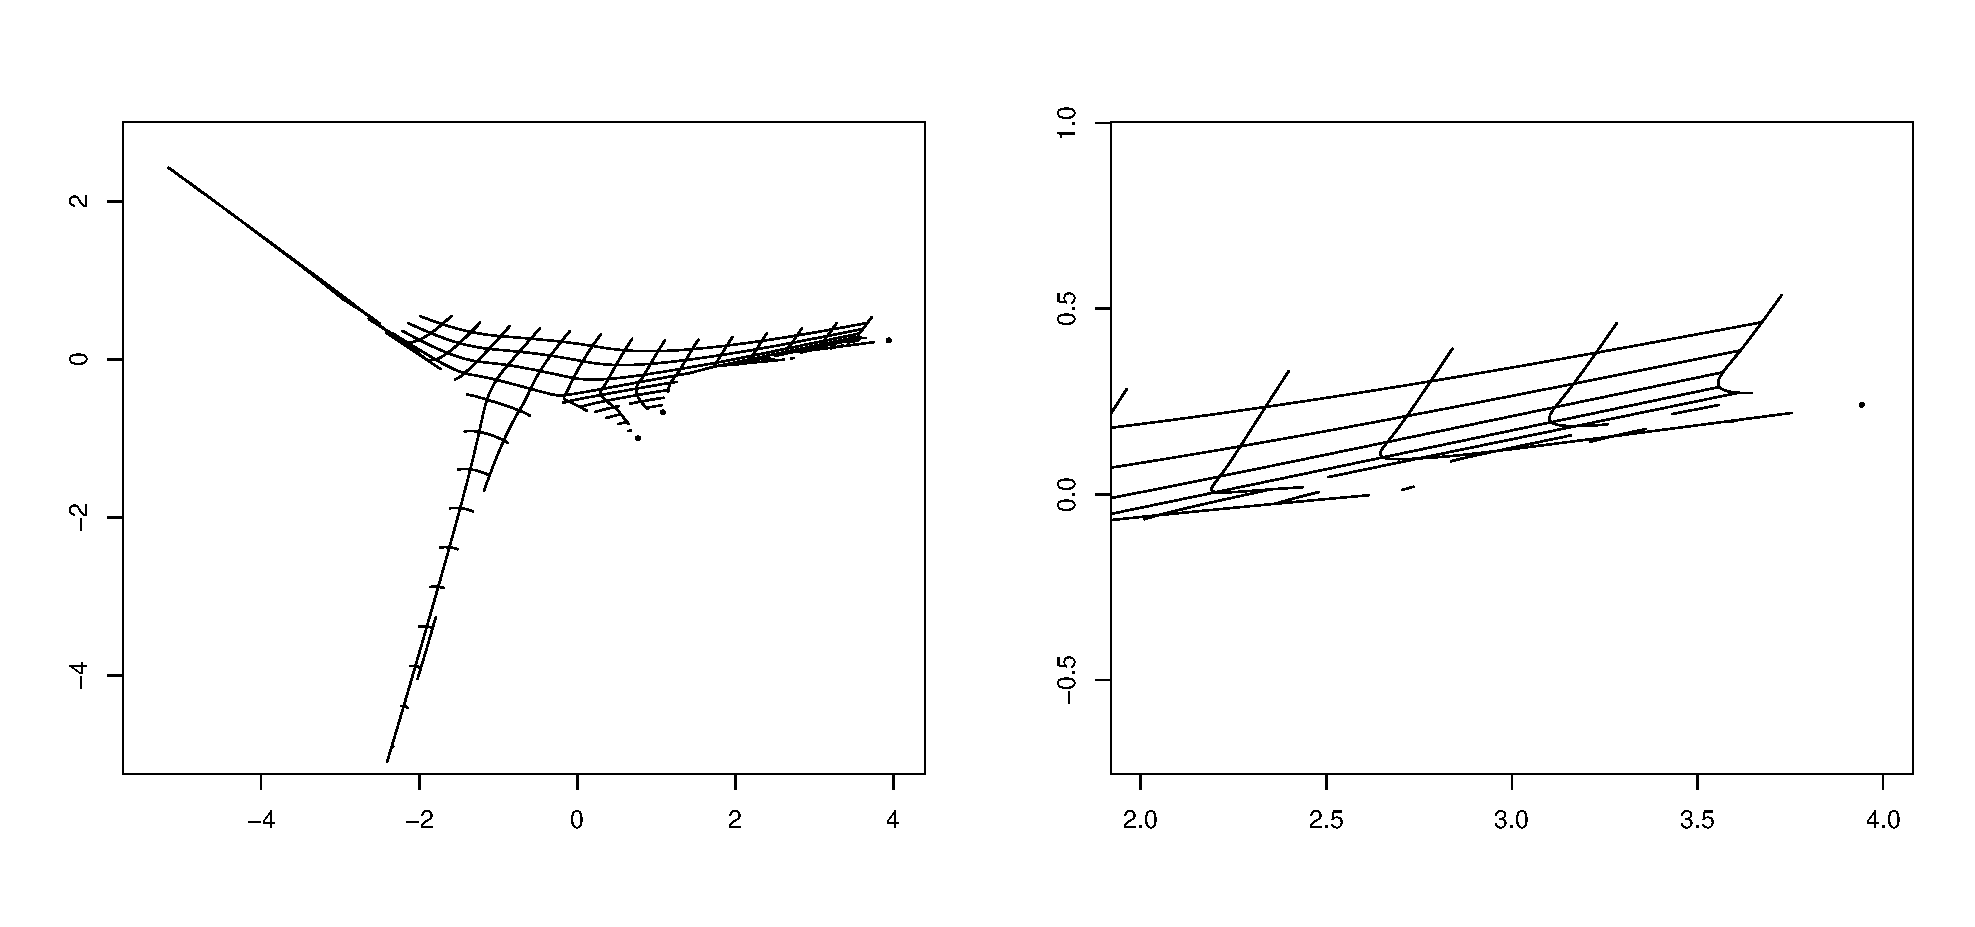
\includegraphics[width=5in]{figs/wt2-grid-full.pdf} \\
\caption{Inserted grid when 1253 points are used to create the initial MDS configuration. The right panel shows a zoom of the far right part of the configuration.}
\label{wt2-grid-full}
% generated using wt2-grid.R
\end{figure}

% mapped grid (samp)
\begin{figure}
\centering
% trim order l b r t
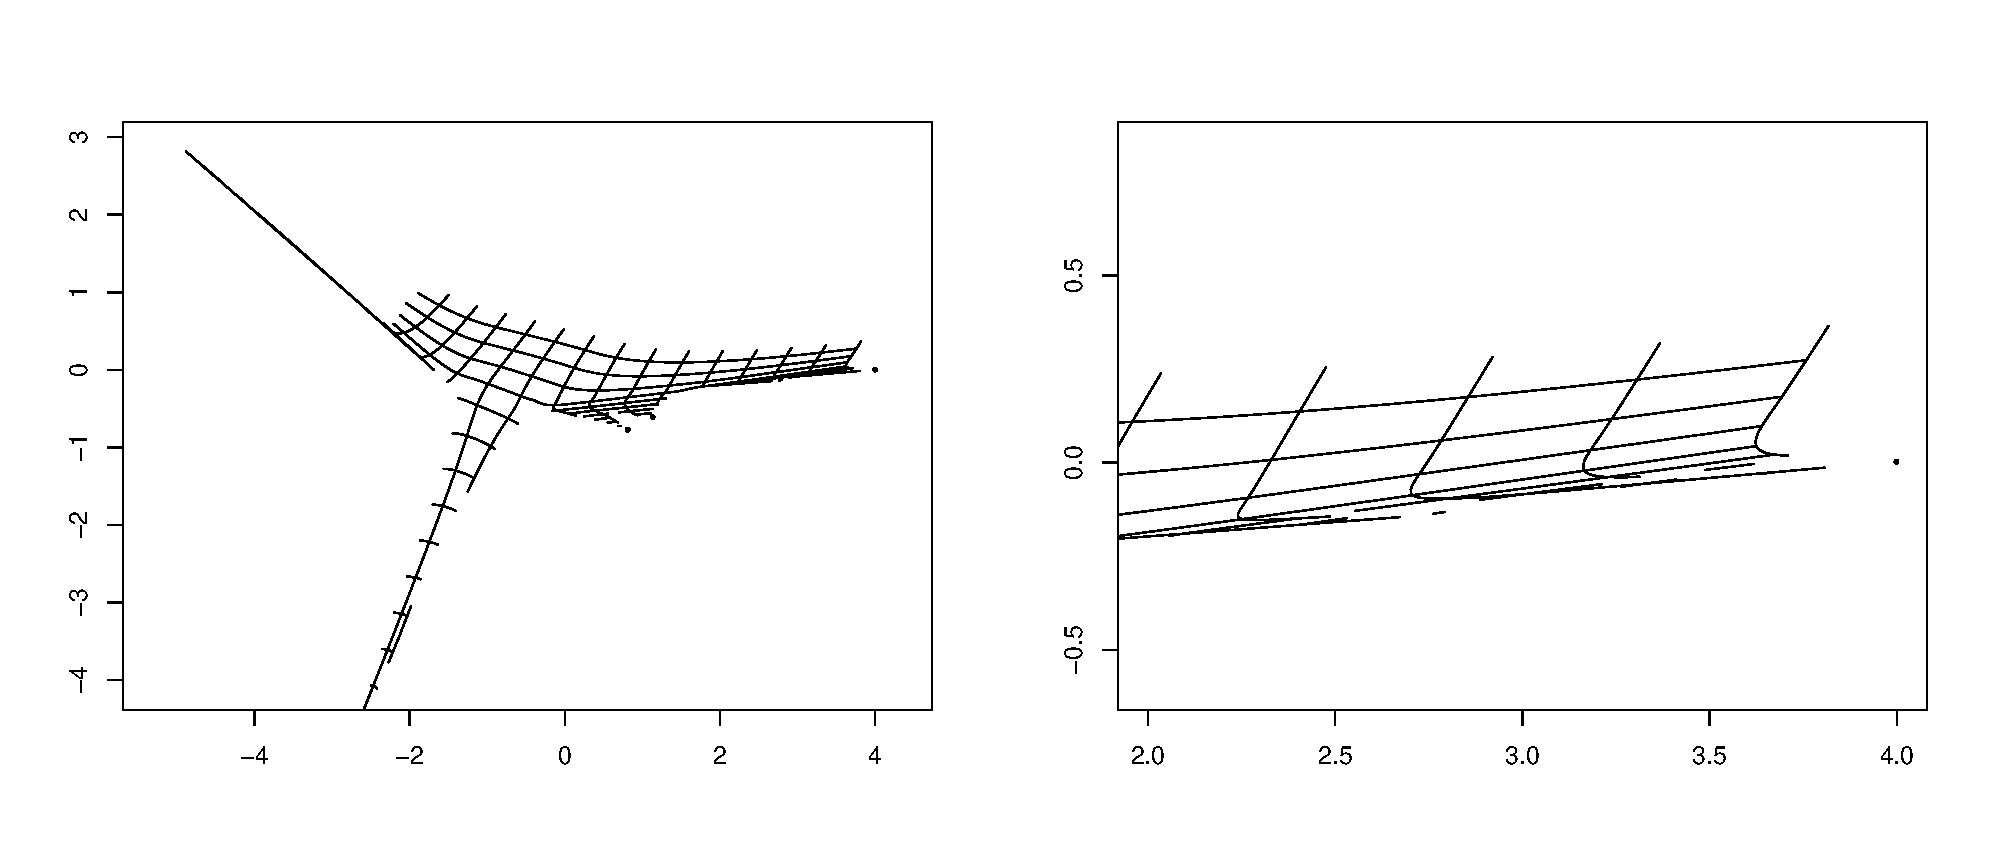
\includegraphics[width=5in]{figs/wt2-grid-samp.pdf} \\
\caption{Inserted grid when 250 randomly chosen points are used to create the initial MDS configuration. The right panel shows a zoom of the far right part of the configuration. Comparing this to that of \fig{wt2-grid-full}, one can see that the right side features have been squashed together.}
\label{wt2-grid-samp}
% generated using wt2-grid.R
\end{figure}

So, here we have seen that the mapping can be both reliable and also produces a smooth configuration of points provided that the initial MDS configuration covers the space in sufficient detail.


\section{Finding the within-area distances}

In order to perform multidimensional scaling the matrix of distances must be first found. In this case it makes sense to find the shortest distances between each pair of points where the path between the points lies entirely within the domain.

Let the domain boundary be some polygon, $\Gamma$. Given that there is no direct path within the domain between two points ($p_1$ and $p_2$, say), the algorithm proceeds as follows to create a path (ie. an ordered set of edges and vertices), $\mathcal{P}$:

\begin{enumerate}
\item (INIT) Start by drawing a line between $p_1$ and $p_2$ (\fig{wdia}, ($i$)). Start the path as the lines from $p_1$, $p_2$ to their nearest intersection with the boundary of $\Gamma$ ($p_1^1$, $p_2^1$, say.) Then form two paths. The first path from $p_1^1$ to $p_2^1$ ($\mathcal{P}_1$) contains the vertices of $\Gamma$ found moving along the boundary from $p_1^1$ to $p_2^1$. The second ($\mathcal{P}_2$), is found by taking those vertices on the boundary from $p_2^1$ to $p_1^1$, ie. the vertices of $\Gamma$ not in the first path. It is easy to see that $\{\mathcal{P}_1 \cup \mathcal{P}_2\} \setminus \{p_1^1, p_2^1\} = \Gamma$. Finding the length of $\mathcal{P}_1$ and $\mathcal{P}_2$ and choosing the shorter ($\mathcal{P^*}$), the initial path is formed as $\mathcal{P}=(p_1,p_1^1,\mathcal{P}^*,p_2^1,p_2)$. 

In \fig{wdia}, ($iii$), $\mathcal{P}_1$ is marked in green and is chosen to form the initial path, $\mathcal{P}=(p_1,p_1^1,\mathcal{P}_1,p_2^1,p_2)$, as $\mathcal{P}_1$ is shorter than $\mathcal{P}_2$, in red.

\item (DELETE) Given a triple of vertices, $(v_i, v_{i+1}, v_{i+2}) \in \mathcal{P}$ , if the line between $v_i$ and $v_{i+2}$ is shorter than the path $(v_i, v_{i+1}, v_{i+2})$ and the line between $v_i$ and $v_{i+2}$ lies inside $\Gamma$ then delete $v_{i+1}$ (\fig{wdia}, ($iv$) and ($vi$).) The entire path is iterated over deleting all superfluous vertices until there are no changes in successive runs. 

For example in \fig{wdia}, ($iii$) $v_2$ is deleted from $\mathcal{P}$ because the path straight between $v_1$ and $v_3$ is shorter, and within $\Gamma$.

\item (ALTER) Given a triple of vertices $(v_i, v_{i+1}, v_{i+2})$, if the path $\mathcal{P}_{ID}$ is shorter than the path $(v_i, v_{i+1}, v_{i+2})$ then replace $(v_i, v_{i+1}, v_{i+2})$ with $\mathcal{P}_{ID}$ (\fig{wdia}, ($v$)). The candidate replacement path, $\mathcal{P}_{ID}$, is calculated by running INIT with $p_1$ and $p_2$ replaced by $v_i$ and $v_{i+2}$, producing $\mathcal{P}_I$, and then using DELETE on $\mathcal{P}_I$ to remove superfluous vertices, giving $\mathcal{P}_{ID}$.

For example in \fig{wdia} ($iv$), the path $(v_1, v_2, v_3)$ is longer than the path $\mathcal{P}_{ID}=(v_1, v^1_2, v_3)$ (green dashed line in ($iv$)) so the former is replaced with the latter in $\mathcal{P}$. The path created by INIT is marked as $\mathcal{P}_{I}$ in  ($iv$) in red.

\item (ITER) We then iterate between the DELETE and ALTER steps until there has been no change from one run to the next (ie. convergence) or there have been too many iterations (\fig{wdia}, ($vi$).)
\end{enumerate}

% diagram for finding the shortest path in W
\begin{sidewaysfigure}
\centering
% trim order l b r t
\psfrag{exp1}[]{$\mathcal{P}_1$}
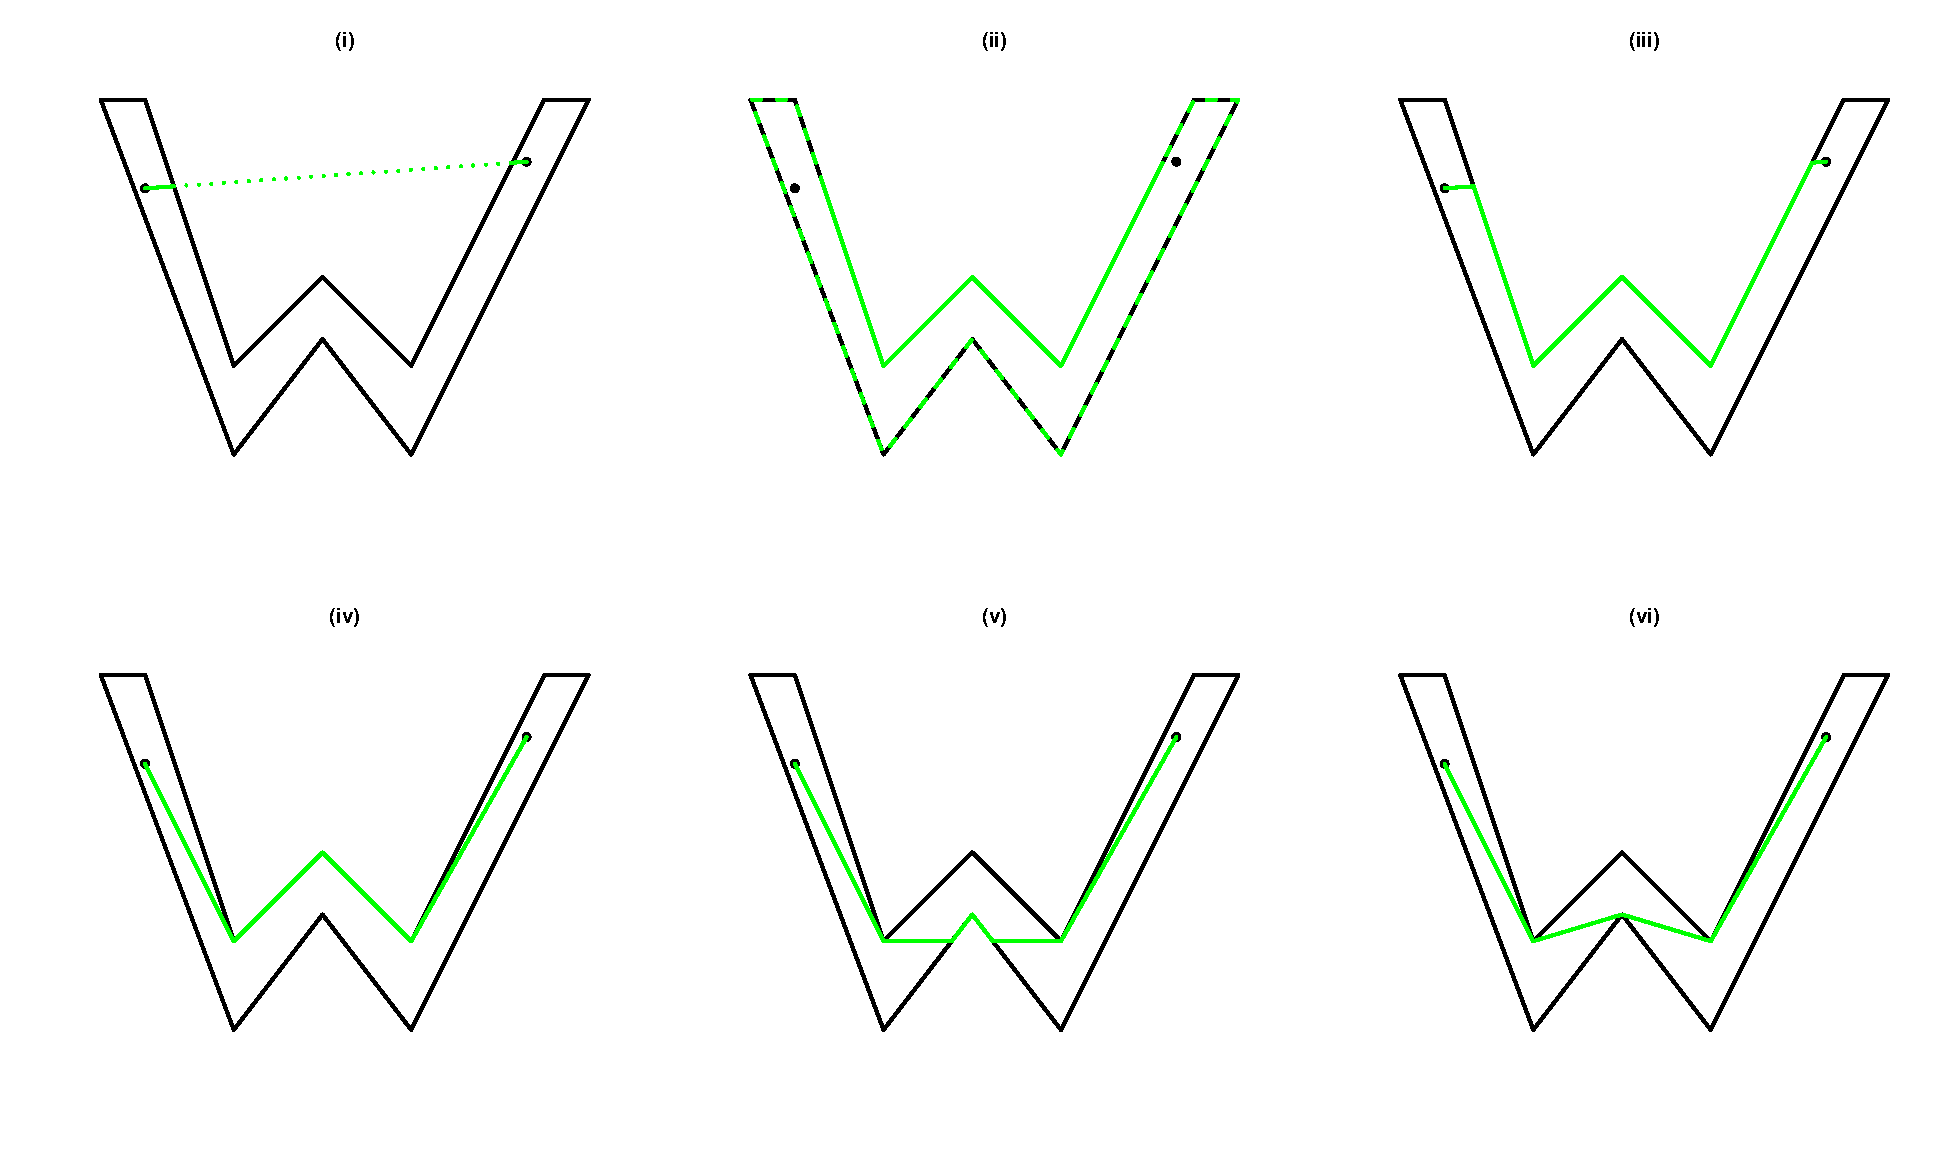
\includegraphics[trim=0in 0.5in 0in 0.25in, width=9.5in]{figs/wdia.pdf} \\
\caption{The green lines in ($i$) to ($vi$) show the steps forming the shortest path as the algorithm progresses from initial state to final, shortest path (bottom right.) }
\label{wdia}
% generate /phd-smoothing/mds-writeup/figs/distanceexplanation.R
\end{sidewaysfigure}

Of course, if there is a direct path between $p_1$ and $p_2$ then the Euclidean distance between the points can be used.

\section{Multidimensional scaling for smoothing over complex domains}

Taking a cue from \cite{soap} simulations were conducted on the so-called modified Ramsay horseshoe and another domain supposed to mimic the shape of a coastline. Results are compared using the mean squared error (MSE) criterion and their estimated degrees of freedom (EDF.)

The mean squared error is defined (as in \cite{simonbook} p. 131) as:

\begin{equation}
\text{MSE}(\hat{f}) = \frac{1}{P} \sum_{j=1}^P (\hat{f}(x_j) - z_j)^2,
\end{equation}
the mean difference between the model ($\hat{f}$) evaluated at the prediction points ($\{x_j : j=1 \dots P\}$) and the true value of the function ($\{z_j : j=1 \dots P\}$.) This gives the MSE per model, since here many realisations are run, the mean of these over all simulations is taken and the standard error is calculated.

The estimated degrees of freedom of a model gives an idea of the complexity of the spline that was fit to the data, the higher the EDF, the more basis functions were used and  the more complex the model.  Since the models used here are penalised, it is the penalty term that controls the overall ``wigglyness'' of the spline and hence the EDF. Although the basis dimension is set in the model this is just an upper bound, the smoothing penalty suppresses parts of the model. Therefore basis dimension is not a major concern provided that it is not set too low (\cite{simonbook}, p. 161.) 


\subsection{Modified horseshoe}

The domain in \fig{leakage} is known as the modified Ramsay horseshoe. It is based on the horseshoe-like shape used in \cite{ramsay} and clearly illustrates the problem of leakage. It differs from the figure in \cite{ramsay} in that a slight curvature in the function along the major axis has been added such that the gradient is not perpendicular to the boundary. This curvature was added in \cite{soap}  in order to avoid the horseshoe function lying in the nullspace of the soap film's penalty, making the problem too easy for a soap film smoother.

For the modified horseshoe, 100 replications of samples of 250 points with normal errors (at 3 levels: 0.1, 1 and 10) were run. From these samples, three models were fitted to the data and predictions over 718 points (including the sample locations) and the mean squared error was calculated between the model prediction and the true function value for the horseshoe. The three models fitted were as follows using the \textsf{R} packages \texttt{mgcv} and \texttt{soap}:

\begin{enumerate}
\item \emph{Thin plate spline}: bivariate thin plate spline with basis size 100.
\item \emph{Soap film smoother}: 32 knots evenly spread over a grid over the domain, cyclic spline on the boundary was of basis size 39.
\item \emph{MDS}: Used a thin plate spline of basis dimension 100. The initial MDS grid was 20 points wide by 10 points tall.
\end{enumerate} 

In all cases smoothing parameter estimation was performed using GCV.

Note that due to time and computational restrictions, the boundary was reduced from the 160 vertex polygon in the \texttt{fs.boundary()} function in \texttt{soap} to a 21 vertex polygon by only using every 8$^\text{th}$ vertex.

\begin{table}[ht]
\centering
\begin{tabular}{c c c c}
 & & MSE & \\ 
$\sigma$ & MDS & Soap film & Thin plate\\ 
\hline
0.1  & 0.0032 (3$\cross10^{-5}$) & 0.0022 (3$\cross10^{-5}$) & 0.0402 (0.0008) \\ 
1  & 0.0436 (0.0015) & 0.0482 (0.0014) & 0.2306 (0.0024) \\ 
10  & 2.0652 (0.1215) & 3.0702 (0.2382) & 3.3713 (0.1133) \\ 
\end{tabular}
\begin{tabular}{c  c c c }
&  & EDF & \\ 
$\sigma$ & MDS & Soap film & Thin plate\\ 
\hline
0.1 & 47.613 (0.3497) & 39.164 (0.26) & 92.5996 (0.1020)\\ 
1  & 8.3828 (0.3452) & 11.868 (0.4010) & 46.607 (0.4238)\\ 
10 & 5.0577 (0.3324) & 5.5863 (0.2876) & 5.9786 (0.2511)\\ 
\end{tabular}
\caption{Mean MSE and estimated degrees of freedom (EDF) for the three models fitted to the modified Ramsay horseshoe function with standard errors (in brackets) over 200 realisations.}
\label{ramsayresultstable}
\end{table}

A typical realisation from the models can be seen from \fig{ramsay-fit-1}, where $\sigma=1$ with a sample size of 250. Both the soap film smoother and MDS have respected the boundary and, even with relatively high noise and low sample size, they reproduce the true function fairly well. The thin plate regression spline, on the other hand, shows leakage as expected. This is reflected in table \ref{ramsayresultstable} where we see that the soap film smoother and MDS perform significantly better in terms of mean squared error. It also seems that the MDS performs better than the soap film when there is a high degree of noise in the data.

The EDFs in table \ref{ramsayresultstable} show that the MDS approach always gives a less complex model than using a thin plate spline, and for the two higher error situations, has a lower EDF than the soap film. Given that this is coupled with a lower MSE, it seems that the MDS approach yields both a more accurate and less complex model for the Ramsay horseshoe when there is high noise.

% Ramsay fit with error=1 
\begin{figure}
\centering
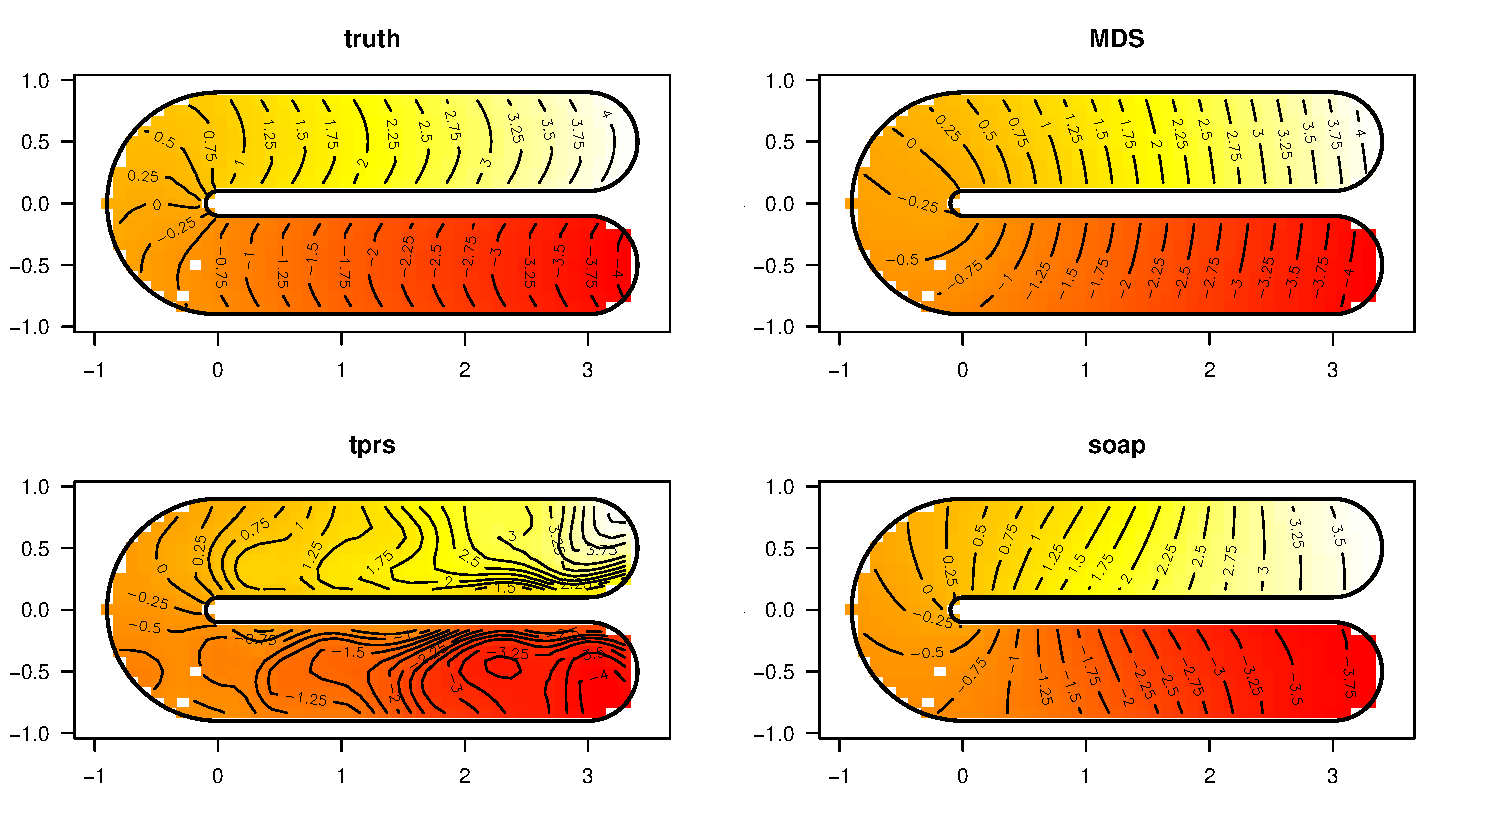
\includegraphics[width=6in]{figs/ramsay-fit-1.pdf} \\
\caption{Top left: truth for the (modified) Ramsay horseshoe. Others: a typical realisation of fits from the three models when 250 points are sampled with noise set to $\sigma=1$.}
\label{ramsay-fit-1}
% generated (roughly) using ramsay-smooth-test.R
\end{figure}

\subsection{Peninsulae domain}

The Ramsay horseshoe is, in a sense, easy domain to smooth over since it is obvious what the transformation should be doing. For this reason a more complex and more realistic domain would provide more insights into the efficacy of the method. The domain shown in \fig{wt2-truth} is an approximation to a coastline with a strong trend along both peninsulae (in a manner similar to that of the horseshoe) but with the added complication of a further peak in the lower right corner.

Again, 200 realisations from the domain shown in \fig{wt2-truth} were used with Normal errors at 3 levels of $\sigma$ (0.05, 0.5 and 5.) Mean squared error over 1253 prediction points (including those points in the sample) was calculated from fitting models with 250 samples. The models fitted were:

% wt2 truth 
\begin{figure}
\centering
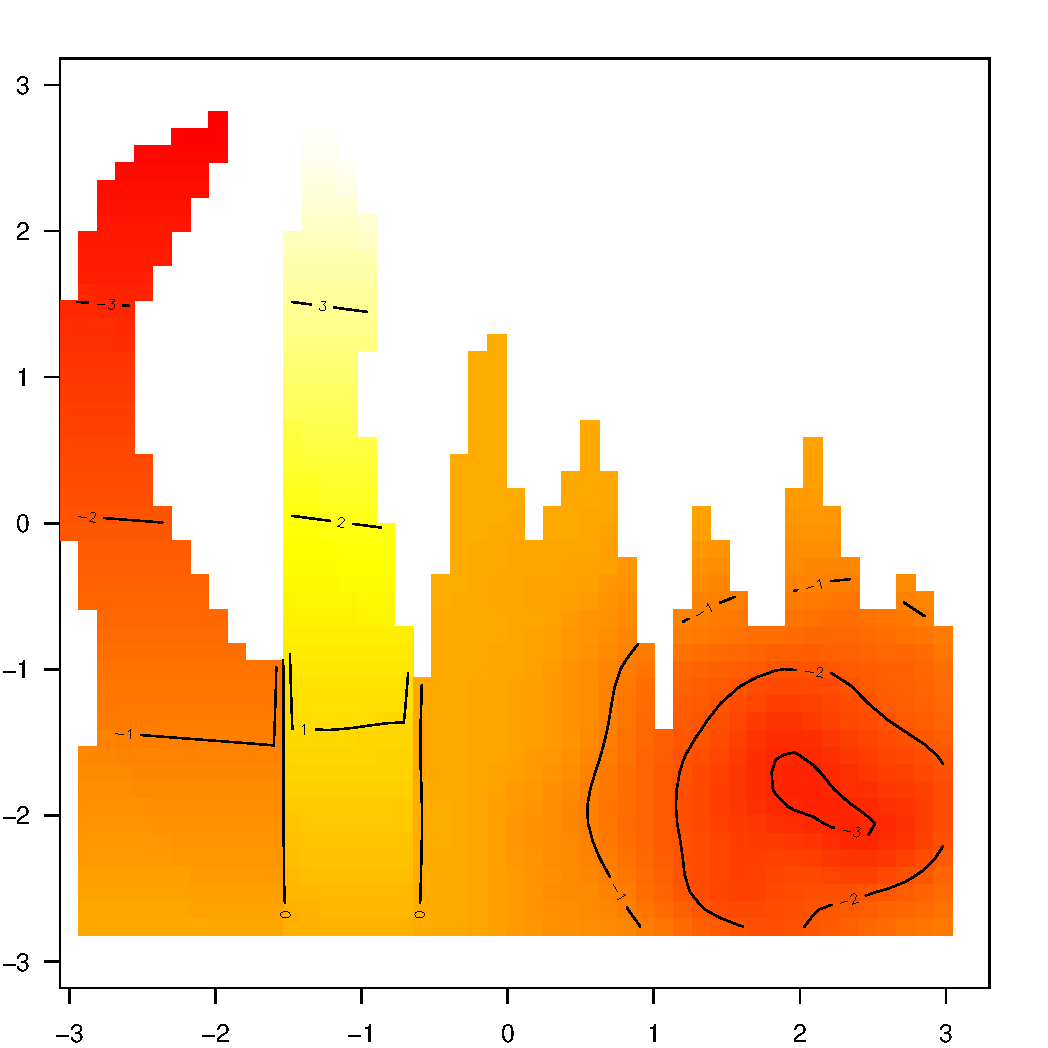
\includegraphics[width=3in]{figs/wt2-truth.pdf} \\
\caption{True function for the domain with multiple peninsulae.}
\label{wt2-truth}
% generated (roughly) using wt2-smooth-test.R
\end{figure}

\begin{enumerate}
\item \emph{Thin plate spline}: bivariate thin plate spline with basis size 100. 
\item \emph{Soap film smoother}: cyclic spline on boundary of basis size 60, 109 internal knots evenly spaced over the domain on a grid.
\item \emph{MDS}: after transform a bivariate thin plate spline with basis size 100 was fit. The initial MDS grid was 74 points square.
\item \emph{MDS with tensor product}: tensor product of two thin plate splines, each of basis dimension 12. The initial MDS grid was 74 points square.
\end{enumerate} 

In all cases smoothing parameter estimation was performed using GCV.

Looking at a typical realisation in \fig{wt2-fit-0.5}, we see that soap (bottom right panel) does very well, as can be expected, and the thin plate spline (\fig{wt2-fit-0.5}, bottom left panel) fit shows leakage (again, as can be expected.) 

The final model, above, was chosen after it appeared that the MDS with a bivariate thin plate spline did not adequately model the peak in the right corner of the domain (\fig{wt2-fit-0.5}, top left panel.) After using a tensor product of thin plate splines a better fit to the right peak was found (\fig{wt2-fit-0.5}, top right panel), although this is not reflected particularly well in terms of mean squared error (see table \ref{wt2resultstable}.) The visual improvement in fit can be explained by thin plate splines in two dimensions being an isotropic smooth and since space has not been transformed in a uniform way in both dimensions.

Table \ref{wt2resultstable} shows that when there is low error, both the soap film and thin plate splines outperform the MDS approach, but once the errors are increased the MDS does much better. The MDS approach also benefits from having a smaller EDF than all the other approaches in all of the noise scenarios, the tensor MDS doing better at lower noise levels. This is encouraging and shows that perhaps there is a place for this technique alongside the soap film smoother if the method can be improved for low noise situations.

\begin{table}[ht]
\centering
\begin{tabular}{c c c c c}
 &  & MSE  & &\\ 
$\sigma$ & MDS & MDS (tensor) & Soap film & Thin plate\\ 
\hline
0.05  & 0.0948 (0.00084) & 0.0603 (0.00352) & 0.0237 (0.00039) &0.0504 (0.00039) \\ 
0.5  & 0.1426 (0.00078) & 0.1106 (0.00133) & 0.1013 (0.02151) &0.1123 (0.02151) \\ 
5  & 0.9179 (0.02644) & 1.2481 (0.04159) & 1.1987 (0.04111) &1.3865 (0.04111)\\ 
\end{tabular}
\begin{tabular}{c c c c c}
 &  & EDF  & &\\ 
$\sigma$ & MDS & MDS (tensor) & Soap film & Thin plate\\ 
\hline
0.05 &72.262 (0.89606) & 78.2691 (0.679) & 94.5187 (0.78697) & 86.9415 (0.78697)\\ 
0.5 &40.7981 (0.46687) & 50.5025 (0.36223) & 45.2341 (0.74063) & 58.418 (0.74063)\\ 
5  &6.8274 (0.36097) & 8.577 (0.3649) & 11.5419 (0.83982) & 11.9407 (0.83982)\\ 
\end{tabular}

\caption{Mean MSE and EDF for the four models fitted to the peninsula domain with standard errors (in brackets) over 200 realisations.}
\label{wt2resultstable}
\end{table}




% wt2 fit with error=0.5
\begin{figure}
\centering
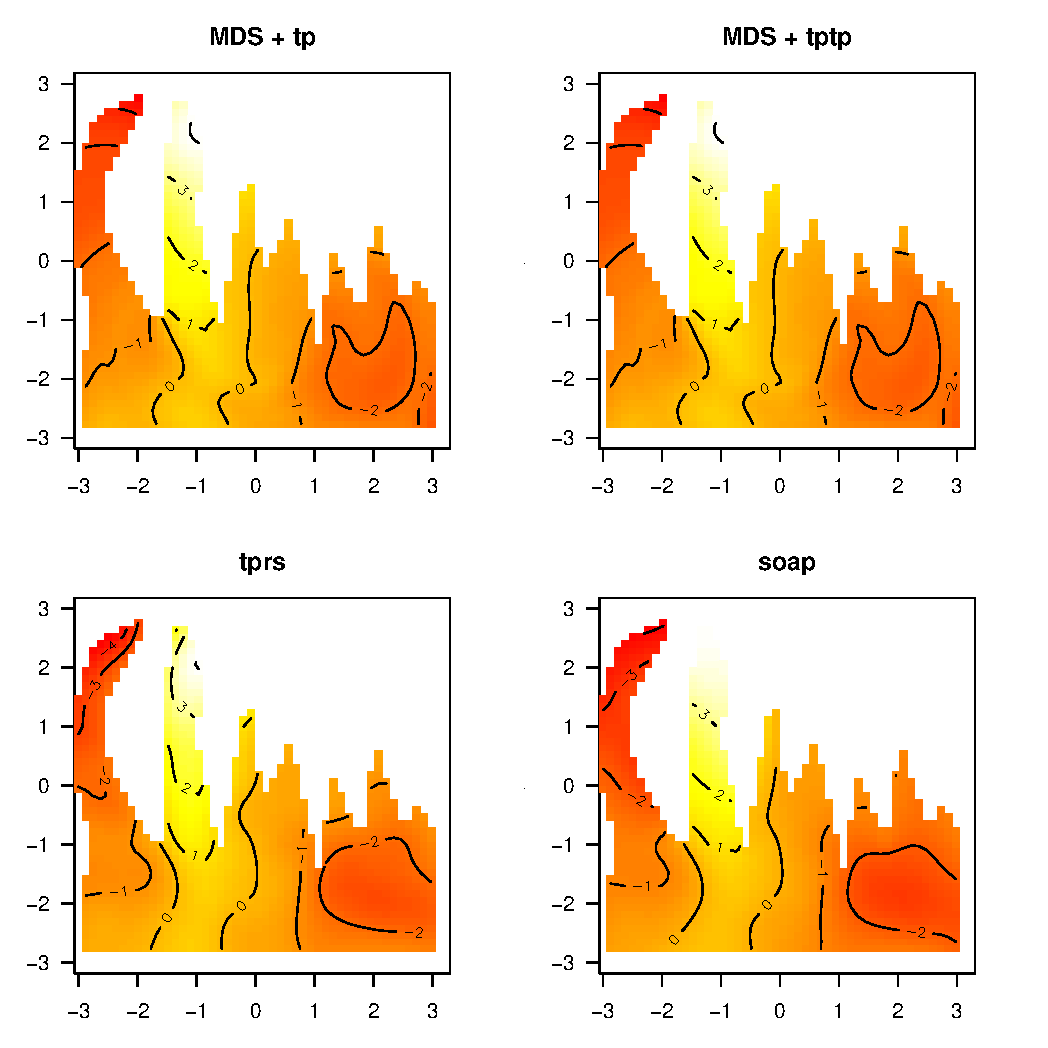
\includegraphics[width=6in]{figs/wt2-fit-05.pdf} \\
\caption{A typical realisation of fits from the multiple peninsulae domain when $\sigma$ is set to 0.5.}
\label{wt2-fit-0.5}
% generated (roughly) using wt2-smooth-test.R
\end{figure}



\section{Conclusions}

Although these results are encouraging, the inability of the smooth to capture all the features in the right side of the domain when using an isotropic smoother is disappointing. Proposed further work is to follow the lead from \cite{wood2000}, which shows that given some transform of a variable, $y$ say, such that $y_i^\prime=y_i/k$, then $f(x,y^\prime k)$ will give the same fit as $f(x,y)$ (ie. the fit will be the same under the new coordinates) but the penalty will change to:
\begin{equation}
\int\int_\Omega \Big( \frac{\partial^2 f}{\partial x^2} \Big) + 2k\Big( \frac{\partial^2 f}{\partial x \partial y} \Big) + k^3\Big( \frac{\partial^2 f}{\partial y^2} \Big) \text{d}x \text{d}y,
\label{adjustedintegral}
\end{equation}
from:
\begin{equation*}
\int\int_\Omega \Big( \frac{\partial^2 f}{\partial x^2} \Big) + 2\Big( \frac{\partial^2 f}{\partial x \partial y} \Big) + \Big( \frac{\partial^2 f}{\partial y^2} \Big) \text{d}x \text{d}y.
\end{equation*}
In the case of the MDS, the integral would need to be split over a grid such that each cell captured the distortion in space over the area of the cell. Mathematically, $\Omega$ would be split into a subsets, $\omega_i$ (where $\bigcup_{\forall j} \omega_j = \Omega$) and (\ref{adjustedintegral}) becomes:
\begin{equation}
\sum_{\forall j} \int\int_{\omega_j} l_j^3 \Big( \frac{\partial^2 f}{\partial x^2} \Big) + 2k_jl_j\Big( \frac{\partial^2 f}{\partial x \partial y} \Big) + k_j^3\Big( \frac{\partial^2 f}{\partial y^2} \Big) \text{d}x \text{d}y,
\end{equation}
where $k_j$ is the scaling in the $y$ direction and $l_j$ is the scaling in the $x$ direction for the $j^{\text{th}}$ cell. We assume here that $f(x,y)$ is ``nice''.

Using this penalty may allow for the distortions in space to be taken account of and therefore get around the problem of the details being smoothed over, as seen above. It will be easiest to first build this using a tensor product of $P$-splines to test its utility (since their penalty is discrete) and then move on to the thin plate spline penalty.

In order to make this MDS approach competitive with \texttt{soap} (assuming that the above distortion adjustment is successful) a speed-up in the computation of the within-area distances must be achieved. At the moment this is the major bottleneck in the calculation since model fitting consists only of fitting a thin plate spline. 


\begin{table}[ht]
\centering
\begin{tabular}{c || c c c}
 & MDS & Soap film & Thin plate\\ 
\hline
Fit & 3.39225 & 10.87688 & 0.61492\\
Prediction & 4.80357 & 8.87535 & 0.10845\\
\end{tabular}
\label{ramsaytime}
\caption{Average time (in seconds) to fit a realisation of the modified Ramsay horseshoe for the three models considered above. Times are averaged over 100 realisations and were found using the elapsed time provided by \textsf{R}'s built-in \texttt{system.time} function.}
\end{table}


\begin{table}[ht]
\centering
\begin{tabular}{c || c c c c}
 & MDS & MDS (tensor) & Soap film & Thin plate\\ 
\hline
Fit & 84.85242 & 85.35168 & 36.24865 & 0.51721\\
Prediction & 155.4004 & 155.2419 & 44.22065 & 0.20994 \\
\end{tabular}
\label{wt2time}
\caption{Average time (in seconds) to fit a realisation of the peninsula domain for the four models considered above. Times are averaged over 100 realisations and were found using the elapsed time provided by \textsf{R}'s built-in \texttt{system.time} function.}
\end{table}


Speed-ups can be achieved by minimizing the number of calculations for within-area distance that are needed. In \cite{landmark} a method to calculate MDS coordinates using a sparse grid of landmark points is suggested; although the authors are sceptical about how this will perform with non-Euclidean distances. There is clearly some work here in finding some minimal set of landmark points for the within-area distance metric obtained from the above algorithm.

The calculation of within-area distances could be linked into a ``landmark''-type process by calculating the within-area distances between a set of points in a sparse grid, then saving those paths. The distances between desired points can then be found by modifying the path with the end points nearest to those of the desired points.


\bibliographystyle{chicago}
\bibliography{mds-refs}

\end{document}


\chapter{Generalized distance smoothing}
%\begin{quotation}
%The three virtues of a programmer:
%\begin{enumerate}
%\item Laziness - The quality that makes you go to great effort to reduce overall energy expenditure. It makes you write labor-saving programs that other people will find useful, and document what you wrote so you don't have to answer so many questions about it. Hence, the first great virtue of a programmer. Also hence, this book. See also impatience and hubris.
%\item Impatience - The anger you feel when the computer is being lazy. This makes you write programs that don't just react to your needs, but actually anticipate them. Or at least pretend to. Hence, the second great virtue of a programmer. See also laziness and hubris.
%\item Hubris - Excessive pride, the sort of thing Zeus zaps you for. Also the quality that makes you write (and maintain) programs that other people won't want to say bad things about. Hence, the third great virtue of a programmer. See also laziness and impatience.
%\end{enumerate}
%-- Larry Wall, Randal L. Schwartz and Tom Christiansen. 
%\end{quotation}
%\begin{quotation}
%``The three virtues of a programmer: laziness, impatience and hubris.''
%
%-- Larry Wall, Randal L. Schwartz and Tom Christiansen. 
%\end{quotation}

% general distance smoothing stuff

\label{chap-gds}


\section{Introduction}

The previous chapter makes clear that there are two conflicting issues impeding the utility of this approach to smoothing over complex regions. The first is that the ordering of the points in space must be maintained, but (second) once a sufficiently high dimensional projection of the data has been obtained, the nullspace of the penalty must be kept as small as possible in order to stop a large space of wiggly function from being fit without being penalised.

Facing the interplay of these two factors, the requirement we seek is clear: we wish to smooth in as many dimensions as possible but while doing this we must also limit the nullspace of the penalty. Fortunately, this is possible using the ideas put forth in \cite{duchon77}. The methods detailed there give a generalisation of the thin plate spline basis that allows for the nullspace to be constrained.

The next section goes into the technical detail of how this approach works. Section \ref{gds-wad-examples} shows how this can be useful in the within-area distance case discussed in chapters \label{chap-sc} and \label{chap-mds}. Section \ref{gds-gds-examples} gives examples of generalized distance smoothing.

\section{Duchon splines}

\cite{simonbook} p. 153 gives the formulation for the thin plate penalty in $d$ dimensions with penalty order $m$ as:
\begin{equation}
J_{m,d} = \int \ldots \int_{\mathbb{R}^n} \sum_{\nu_1 + \dots + \nu_d=m} \frac{m!}{\nu_1! \dots \nu_d!}\Big( \frac{\partial^m f(x_1,\dots,x_d)}{\partial x_1^{\nu_1} \ldots  \partial x_d^{\nu_d}} \Big)^2 \text{d} x_1 \ldots  \text{d} x_d,
\label{tprs-pen}
\end{equation}
where the summation index can be interpreted as all of the possible combinations of penalty orders such than their sum is still $m$. The restriction $2m>d$ is also imposed. Although $m$ may be as small as $d/2$, as $d$ gets larger, $m$ is still going to be quite big.

\cite{duchon77} suggests using the Fourier transform of the derivatives in the penalty, thus penalising those second derivatives that have particularly high frequencies (which one can think of as equivalent to penalising the wiggly parts of the function, as in (\ref{tprs-pen})). Duchon then goes on to suggest putting a weighting factor in the integral. 

The Fourier transform decomposes functions into their frequency domain representations (from $\mathbf{x}$ to $\boldsymbol{\tau}$). The Fourier transform of some function, $g$, is defined in the usual way:
\begin{equation*}
\mathfrak{F} g(\boldsymbol{\tau}) = \int_{\mathbb{R}^n} e^{2 \pi \sqrt{-1} \mathbf{x}^\text{T} \boldsymbol{\tau}} g(\mathbf{x}) \text{d}\mathbf{x}.
\end{equation*}
Here $\mathfrak{F}$ is an operator applied to $g$, so $\mathfrak{F}g$ may be considered as a function of $\boldsymbol{\tau}$ (an $n$-vector which characterizes the frequencies). More detail on Fourier transforms can be found in (for example) \cite{bracewell}. 

The penalty proposed by Duchon can be written (in the above notation) as:
\begin{equation*}
\breve{J}_{m,d} = \int \ldots \int_{\mathbb{R}^n} \lvert \boldsymbol{\tau} \rvert^{2s} \sum_{\nu_1 + \dots + \nu_d=m} \frac{m!}{\nu_1! \dots \nu_d!}\Big( \mathfrak{F} \frac{\partial^m f}{\partial x_1^{\nu_1} \ldots  \partial x_d^{\nu_d}}(\boldsymbol{\tau}) \Big)^2 \text{d} \boldsymbol{\tau}.
\end{equation*}
Duchon shows that since the Fourier transform is isometric on $\mathcal{L}^2(\mathbb{R}^n)$, $J_{m,d} = \breve{J}_{m,d}$ when $s=0$ (this result is known as Plancherel's theorem). Duchon chooses the weighting function $\lvert \boldsymbol{\tau} \rvert^{2s}$ due to its invariance to translation and rotation (here $\lvert \cdot \rvert$ is the Euclidean norm).

When $s>0$ higher frequencies are penalised more than lower ones. In order to obtain smooth functions it is required that $m+s>d/2$. So, $s$ can be used to allow smoothing in high dimensional spaces, using lower-order penalties whilst still yielding continuous results.

Using the above results it is then possible to use $m=2$ for smoothing in any dimension ($d$) by changing the value of $s$. Indeed, the inequality relating the three quantities can be seen as a guide for choosing $s$, given some fixed values of $d$ and $m$:
\begin{equation*}
d/2 -m \leq s,
\end{equation*}
so, letting:
\begin{equation}
s=d/2-2,
\label{duchon-s}
\end{equation}
does not seem unreasonable. Here $d$ is the dimension of the MDS projection (ie. the dimension in which we are smoothing). 

One can calculate the size of the nullspace of a thin plate spline:
\begin{equation*}
M=\begin{pmatrix} m+d-1 \\ d  \end{pmatrix},
\end{equation*}
(see \cite{wood2003}, p. 97).

Figure \ref{nullspace-dim} shows a comparison between the nullspace dimension for thin plate regression splines (\textit{a la} \cite{wood2003}) (in blue) and Duchon splines when $s$ is set as in (\ref{duchon-s}) (in red). As can be seen in the graphic, there is a big difference in the nullspace dimension between the two bases even when the smoothing dimension is fairly small.

\begin{figure}
\centering
\includegraphics[width=3in]{mds/figs/nullspace-dim.pdf} \\
\caption{Relationship between smoothing dimension ($d$) and the nullspace dimension ($M$) for thin plate regression splines (blue) and Duchon splines (red).}
\label{nullspace-dim}
% generated by thesis/mds/figs/nullspace-dim.R
\end{figure}

\section{Choosing MDS projection dimension}

With Duchon's basis in mind, it is now possible to smooth a space of any dimension using an order 2 penalty, simply by picking $s$ appropriately. Picking the dimension of the MDS projection is now a concern since there is no reason to believe that simply going to higher and higher dimensions will yield better and better results. Keeping in mind the desire for a simple model, it would be preferable to keep the dimension of the projection as small as possible.

\subsection{Using proportion of variation explained}

It is clear that as higher and higher projections are used, a larger and larger proportion of the variation in the distance matrix is explained. It therefore seems reasonable to base the choice of dimension on the proportion of the variation explained in the initial grid. However, what proportion should be used? 80\%? 90\%? 99\%? There is no reason to choose any one of these over the others. Setting the proportion of variation to be explained generally is surely a bad idea, since what works for one domain may well be a disaster for another.


\subsection{Using GCV scores}

Since fitting a GAM with a Duchon spline basis is relatively cheap compared to the cost of finding the within-area distances, the GCV score can be used to find an optimal dimension for the MDS projection. So, using this to our advantage, a series of projections can be tried, their GCV scores calculated, and the best selected as the projection to use for the model.

In particular, starting from a 2-dimensional projection, the dimensionality is increased  and models fitted, until there i an increase in GCV score. The upper bound is the number of dimensions that explain 95\% of the variation in the distance matrix of the initial grid (see section \ref{mds-prac}).  This favours simpler models (in dimensionality terms), although of course a full search can be performed if there is some prior belief that the dimensionality should be higher (indeed there is no reason to believe that the GCV score should be unimodal in dimension). Simulations show that the minima in the GCV score and MSE are in agreement.

Figure \ref{wt2-gcv-projdim-boxplot} shows a plot of GCV score and mean squared error for 60 simulations from the peninsula domain, for each of the 60 realisations a [[new NAME]] was fitted using a 2 through 20 dimensional projection. The boxplots are grouped according to the dimension of the MDS projection used. The graph shows that there is a minima in the score when the dimension is four which corresponds with the minimum MSE.

\begin{figure}
\centering
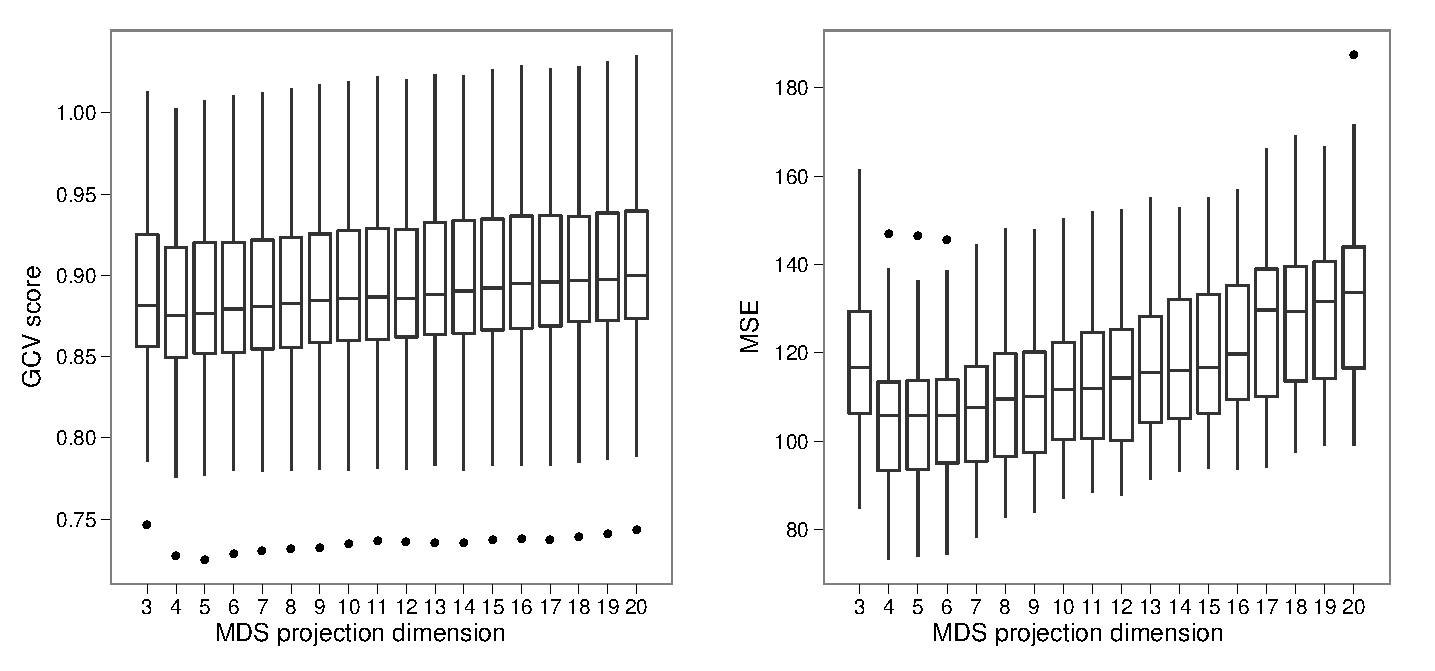
\includegraphics[width=6in]{mds/figs/wt2-gcv-projdim-boxplot.pdf} \\
\caption{MSE and GCV score for the wiggly top domain when different dimensional projections are used. Here a 4-dimensional projection gives a minimum GCV score and MSE.}
\label{wt2-gcv-projdim-boxplot}
% generated by mds/duchon/wt2-gcvml.R
\end{figure}

There is, of course, no guarantee that there will always be a minimum to find and as with all automated methods, practitioners should be mindfull of what could potentially go wrong. However, in the situations tested, this method appeared to be satisfactory.

\section{Within-area distance examples}
\label{gds-wad-examples}
\subsection{Simulations}

Returning to the simulation study in section \ref{wt2bigsim}, the same set of simulations (250 samples at three error levels) was re-run but now using the Duchon splines, selecting MDS dimension based on GCV score (maximum basis dimension was set at 100). The results are shown for the original simulations along side those for the new model (those models which did not to very well originally are excluded).

Figure \ref{wt2-boxplot-duchon} shows the boxplots for these simulations, the [[GIVE THIS A NAME]] method does better than the soap film smoother when the noise is low and was indistinguishable (via a paired Wilcoxon signed rank test) from the soap film smoother at higher noise levels.

\begin{figure}
\centering
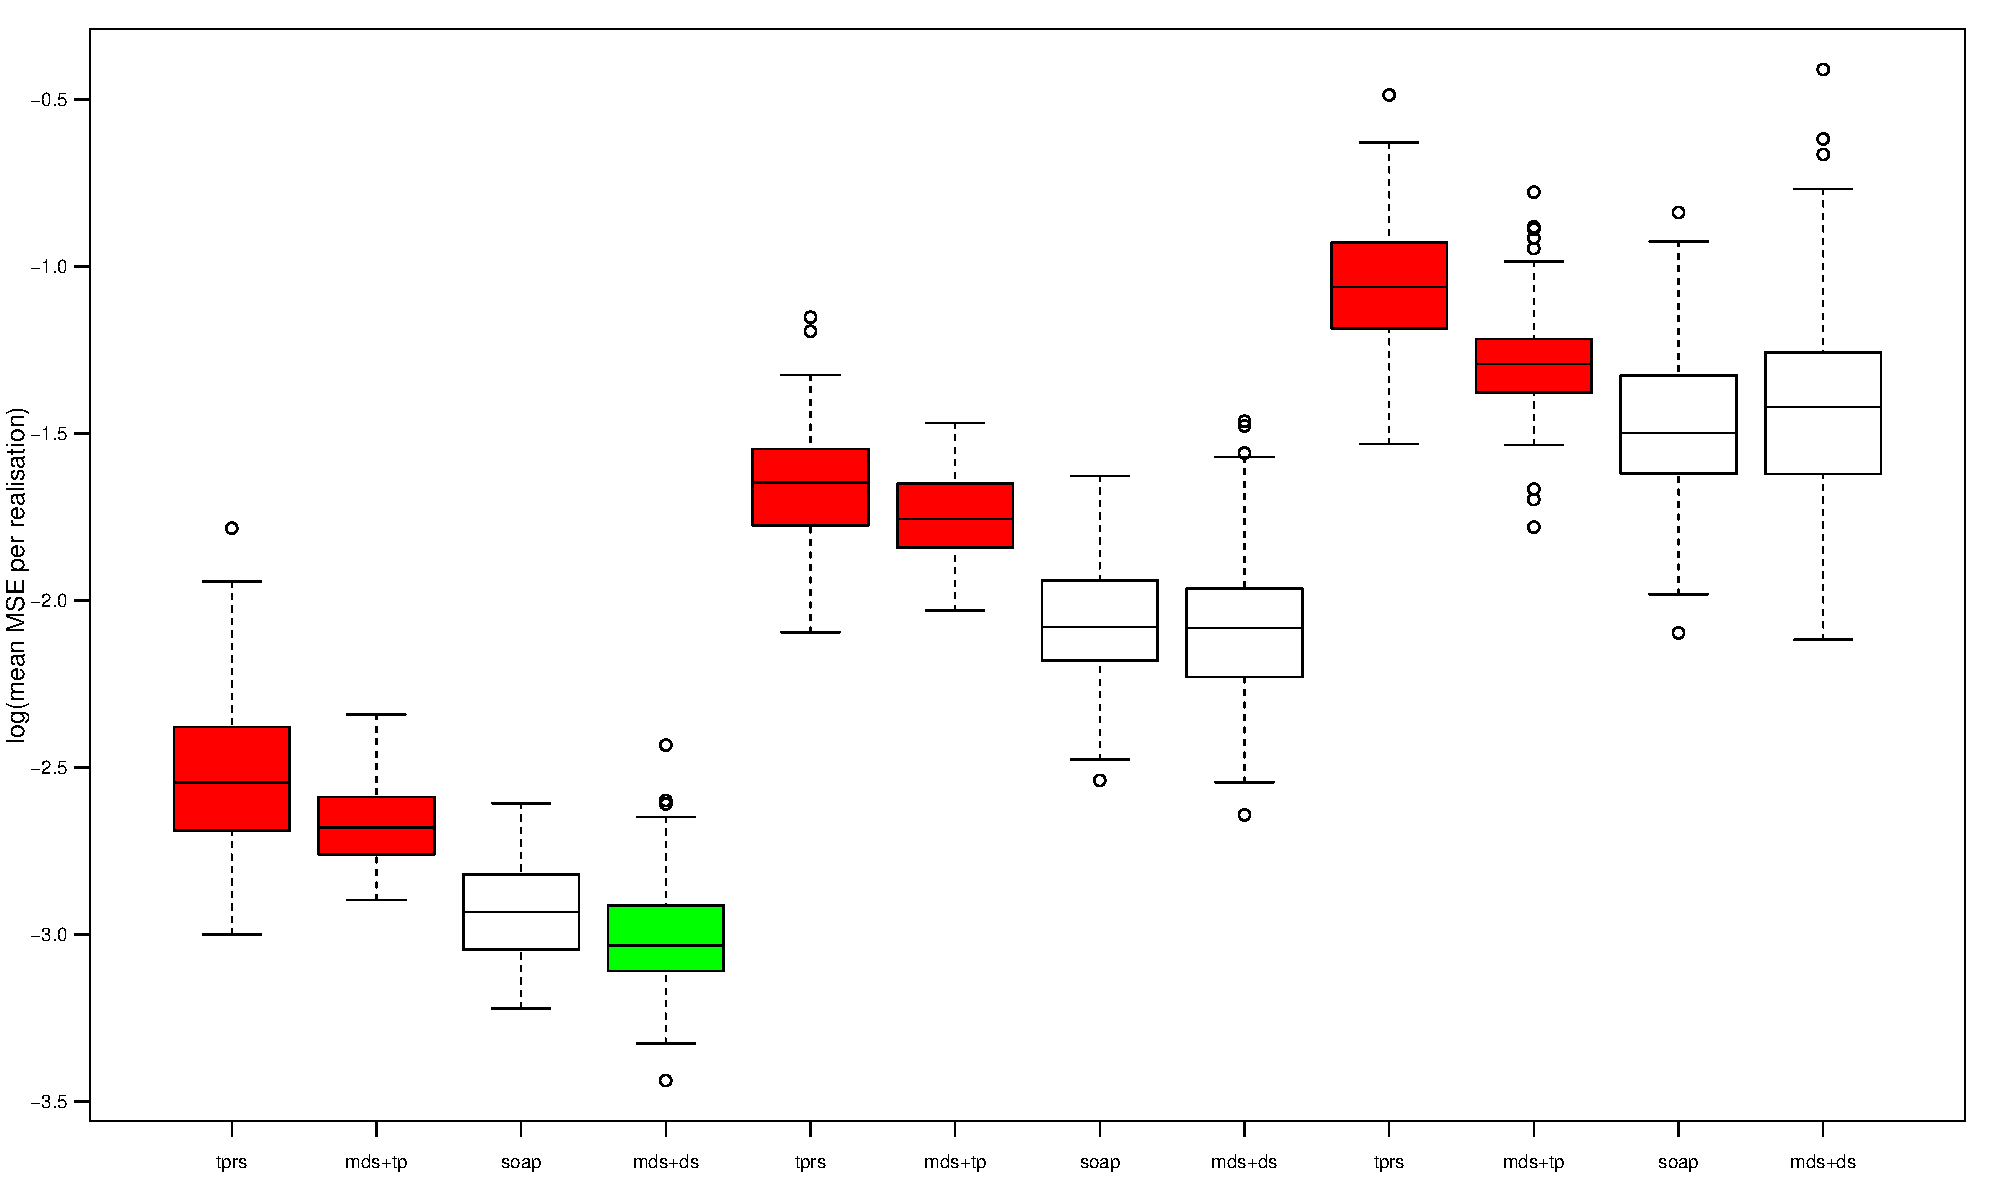
\includegraphics[width=6in]{mds/figs/wt2-boxplot-duchon.pdf} \\
\caption{Boxplots of logarithm of per realisation average mean squared error from simulations on the wiggly top domain. The boxplots are in groups of four for each error level $(\sigma = 0.35, 0.9, 1.55)$. Colours indicate the result of a Wilcoxon paired signed rank test of whether the MSE was significantly (p$<10^{-2}$) different from the soap film smoother. Red indicates different and worse, green different and better.}
\label{wt2-boxplot-duchon}
% generated by mds/duchon/bigsim/boxplot-wt2.R
\end{figure}

[[new wt2??]]

[[aral sim as before?]]

[[ramsay??]]



\subsection{Revisiting the Aral sea}

Going back to the Aral sea example from section \ref{aral-sec}, we can fit a model using the optimal (in a GCV score sense) dimension. Figure \ref{mds-aral-5d-duchon} shows the raw data and a smoothed version, using a 5-dimensional projection (given by minimising the GCV score). The plot does not contain any of the artefacts that were present in the previous smooths of the data.

\begin{figure}
\centering
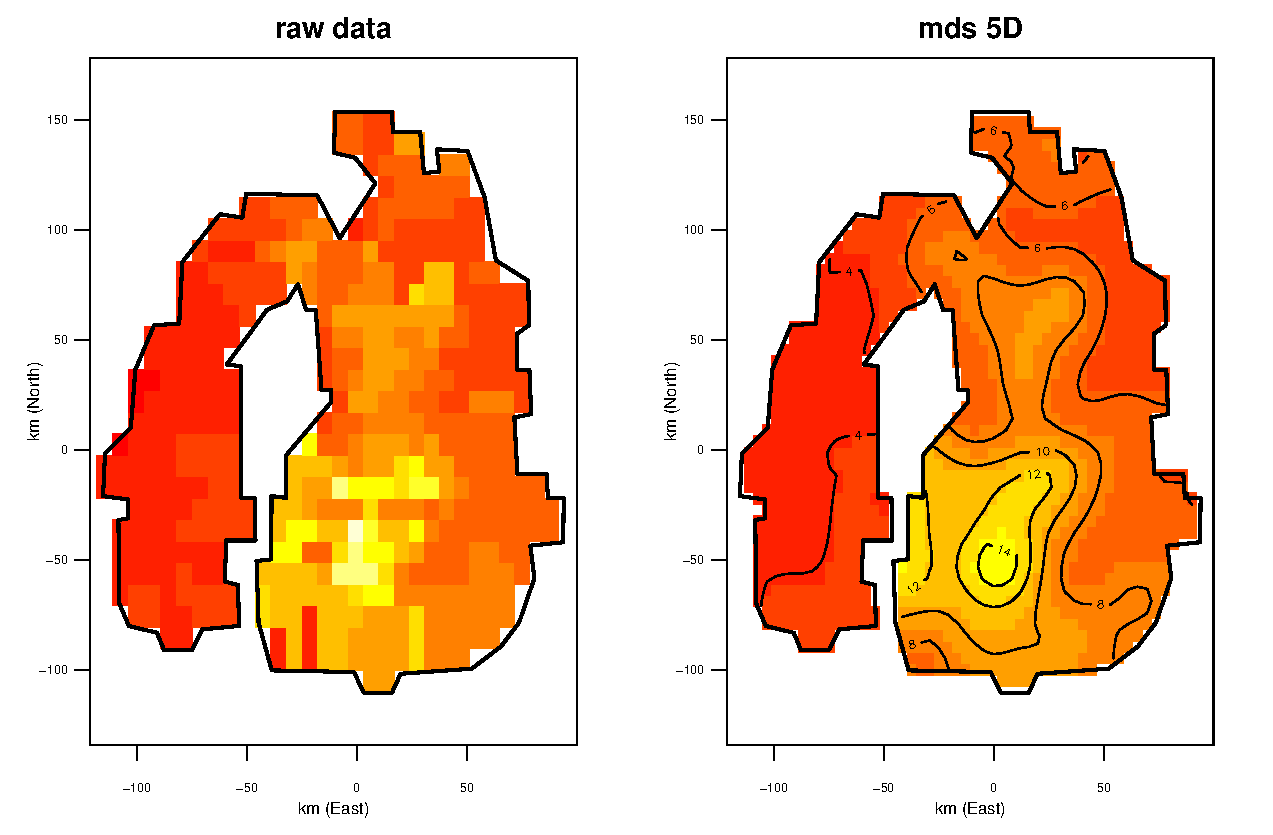
\includegraphics[width=6in]{mds/figs/aral-5d-duchon.pdf} \\
\caption{The Aral sea chlorophyl levels smoothed using Duchon splines, when a 5-dimensional MDS projection is employed. Note the lack of artefacts in comparison to previous \mdsap\ models.}
\label{mds-aral-5d-duchon}
% generated by duchon/aral-evolve.R
\end{figure}



\section{Generalized distance smoothing}
\label{gds-gds-examples}

\subsection{Software implementation - \mdspack}

The methods detailed in this section, namely the use of Duchon splines along with MDS to perform smoothing are provided in the \textsf{R} package \mdspack\ which is available at A WEBSITE THAT MIGHT BE CRAN.


\rule{6in}{1pt}

\rule{6in}{1pt}




\chapter{Mixture model distance sampling detection functions}
% "it's another laser in your intergalactic battle cruiser" - Len Thomas

\section{Introduction}

Repeat what was in the intro a bit

Why do this?

say something about \texttt{mmds}


Do I need to say something about Len here?


%%%%%%%%%%%%%%%%%%%%%%%%%%%%%%%%%%%%%%%%%%%%%%%%%%%
\section{General formulation}

This section lays out, mathematically, the mixture model formulations that can be used for distance sampling detection functions. Beginning with the simplest case (line transects with no covariates) the models are built up and it is shown that the simpler models are just special cases of the more complex ones, thus providing a general framework for mixture model detection functions.

The core principle here is to replace the ``key function plus adjustment terms'' model for the detection function with a mixture model. The simplest example would be to define $g$ as some finite weighted sum of $J$ half-Normal distributions:
\begin{equation}
g(x;\bm{\sigma},\bm{\pi}) = \sum_{j=1}^J \pi_j \exp \Big( \frac{-x^2}{2 \sigma_j^2}\Big).
\label{mmds-simplemix}
\end{equation}
Where the mixture proportions, $\pi_j$, have the property $\sum_{\forall j}\pi_j=1$ and $\bm{\pi} = (\pi_1, \dots, \pi_J)$. $\bm{\sigma}=(\sigma_1,\sigma_2,\dots,\sigma_J)$ are scale parameters. An example of a 2-point mixture of half-Normals is given in figure \ref{2ptdia}.

\begin{figure}
\centering
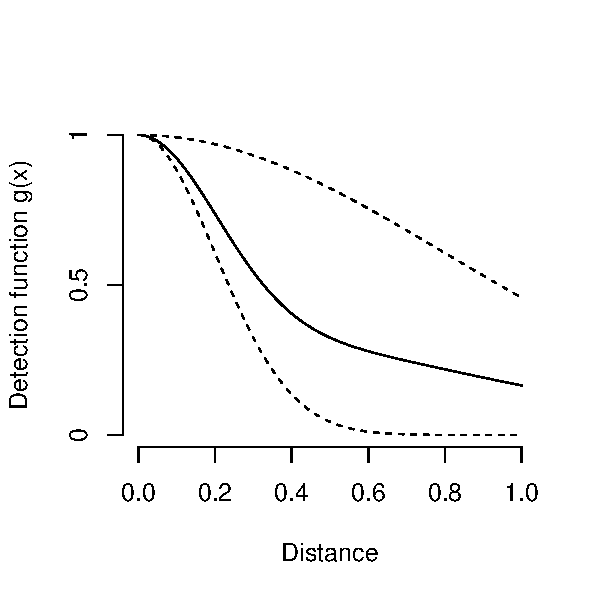
\includegraphics[width=3in]{mix/figs/2ptdia.pdf}
\caption{An example of a 2-point mixture of half-Normals. The two constituent mixture parts are shown with dashed lines, the whole mixture function is the solid line. The scale parameters for the Normal distributions are $0.8$ and $0.2$. The associated mixture proportions are $0.64$ and $0.36$.}
\label{2ptdia}
\end{figure}

Clearly one can think of more complex versions of this: different functions, continuous mixtures or a finite mixture of continuous and finite mixtures (\textit{a la} \cite{morgan08}). However, here only the finite mixture case with half-Normal key functions is considered.

\subsection{Line transects}
For line transects, we can simply substitute equation (\ref{mmds-simplemix}) into the line transect likelihood in equation (\ref{ds-lt-likelihood}). Before doing this we first note that the definition of $\mu$ has not changed, merely the definition of $g$:
\begin{align*}
\mu = \int_0^w \sum_{j=1}^J \pi_j g_j(x;\sigma_j) \text{d}x = \sum_{j=1}^J \pi_j \int_0^w  g_j(x;\sigma_j) \text{d}x = \sum_{j=1}^J \pi_j \mu_j.
\end{align*}
So, the likelihood becomes:
\begin{align}
\mathcal{L}(\bm{\sigma}, \bm{\pi}; \bm{x}) &= \prod_{i=1}^n f(x_i;\bm{\sigma}, \bm{\pi}),\\
&= \prod_{i=1}^n \frac{g(x_i;\bm{\sigma}, \bm{\pi})}{\mu},\\
&= \prod_{i=1}^n \frac{\sum_{j=1}^J \pi_j \exp \Big( \frac{-x_i^2}{2 \sigma_j^2}\Big)}{\sum_{j=1}^J \pi_j \int_0^w  g_j(x;\sigma_j) \text{d}x}.
\label{mmds-lt-likelihood}
\end{align}
which we can obviously think of alternatively as:
\begin{align}
\mathcal{L}(\bm{\sigma}, \bm{\pi}; \bm{x}) &= \prod_{i=1}^n f(x_i;\bm{\sigma}, \bm{\pi}),\\
&= \prod_{i=1}^n \sum_{j=1}^J \pi_j f_j(x_i;\bm{\sigma}, \bm{\pi}),\\
&= \prod_{i=1}^n \sum_{j=1}^J \pi_j \frac{\exp \Big( \frac{-x_i^2}{2 \sigma_j^2}\Big)}{\int_0^w  g_j(x;\sigma_j) \text{d}x}.
\label{mmds-lt-likelihood-pdf}
\end{align}

\subsection{Point transects}
The detection function is, of course, the same for point transects as for line transects. What changes is the PDF and hence likelihood. The likelihood is therefore given as:
\begin{align}
\mathcal{L}(\bm{\sigma}, \bm{\pi}; \bm{r}) &= \prod_{i=1}^n f(r_i;\bm{\sigma}, \bm{\pi}),\\
&= \prod_{i=1}^n \sum_{j=1}^J \pi_j f_j(r_i;\bm{\sigma}, \bm{\pi}),\\
&= \prod_{i=1}^n \sum_{j=1}^J \pi_j \frac{r_i \exp \Big( \frac{-r_i^2}{2 \sigma_j^2}\Big)}{\int_0^w r  g_j(r;\sigma_j) \text{d}r}.
\label{mmds-pt-likelihood-pdf}
\end{align}
where we can define a per-mixture effective area of detection:
\begin{equation}
\nu_j=\int_0^w r  g_j(r;\sigma_j) \text{d}r,
\end{equation}
which is analogous to $\mu_j$, above.

Having these two likelihoods written down, the formulation for covariate models and the generalised likelihood can be derived.

\subsection{Covariate models}
The above models show that the differences between the CDS and mixture model DS (MMDS) are fairly minimal. For the covariate case things are a little more tricky. There are many possible model formulations and the notation is therefore more complicated.

For simplicity of notation, we consider the case where one distance, $x$ (alternatively $r$ for point transects), has been observed and a set of corresponding covariates $z_1,\dots,z_K$ have been recorded too. As before $\sigma_j$ is a (link) function of these covariates and a set of coefficients, the detection function is then defined as:
\begin{equation*}
g(x, \bm{z};\bm{\beta},\bm{\pi}) = \sum_{j=1}^J \pi_j \exp \Big( \frac{-x^2}{2 \sigma_j(\bm{z};\bm{\beta}_j)^2}\Big),
\end{equation*}
defining $\sigma_j(\bm{z};\bm{\beta}_j)$ to be,
\begin{equation*}
\sigma_j(\bm{z};\bm{\beta}_j) = \exp \Big(\beta_{0j} + \sum_{k\in K_j} \beta_{kj} z_k \Big),
\end{equation*}
where $\bm{z}$ is the $K$-vector of all covariates. $K_j$ is the set of covariates to be used with mixture $j$. The vector of per mixture coefficients is $\bm{\beta}_j=(\beta_{0j},\{ \beta_{kj} : k \in K_j\})$. Finally $\bm{\beta}=(\bm{\beta}_1,\dots,\bm{\beta}_J)$ is the vector of all coefficients ordered by mixture part then covariate.

When we have multiple observations we store the distances in $\bm{x}$ (an $n$-vector). Then, for each observation we have a $\bm{z}_i$ and $Z$ is an $n \cross K$ matrix of the covariates for each observation (ie. the $\bm{z}_i$s stacked on top of each other. So then $z_{ik}$ would be the $i^\text{th}$ observation's covariate $k$ (and the $ik^\text{th}$ element of $Z$).

\subsubsection{Covariates - intercept model}

One can think of a special case of the model above when the parameters estimated are common across all mixture parts, except for an intercept.  Mathematically,
\begin{align*}
\sigma_j(\bm{z};\bm{\beta}_j) = \exp \Big(\beta_{0j} + \sum_{k\in K_j} \beta_{k} z_k \Big)
\end{align*}
so the $\beta_{0j}$s are estimated in each mixture but the $\beta_{k}$s are common to all mixtures and are estimated simultaneously. In this case, the $K_j$s are the same for all mixture components.

NOT CURRENTLY IMPLEMENTED

\subsection{Generalised likelihood}
\label{ds-genlik}

\subsubsection{Line transects}
Considering the non-covariate case as a special case of the covariate model, the likelihood can then be written as:
\begin{align}
\mathcal{L}(\bm{\beta}, \bm{\pi} ; \bm{x}, Z) &= \prod_{i=1}^n f(x_i;\bm{\sigma}(\bm{\beta},Z)),\\
&= \prod_{i=1}^n \frac{g(x_i;\bm{\sigma}(\bm{\beta},Z))}{\mu(Z)},\\
&= \prod_{i=1}^n \sum_{j=1}^J \pi_j \frac{g_j(x_i; \sigma_j(\bm{z}_i;\bm{\beta}_j))}{ \mu_j(\bm{z}_i)}.
\label{mmds-lt-glikelihood}
\end{align}
where the $\sigma_j(\bm{z}_i;\bm{\beta}_j)$s take the covariate form above; in the case of a no covariate model, there is only the intercept term, $\beta_{0j}$ ie:
\begin{equation}
\sigma_j = \exp ( \beta_{0j} ).
\end{equation}

\subsubsection{Point transects}
For point transects the likelihood is similar, though with the $r$ pre-multiplier as seen for CDS and MCDS:
\begin{align}
\mathcal{L}(\bm{\beta}, \bm{\pi} ; \bm{r}, Z) &= \prod_{i=1}^n f(r_i;\bm{\sigma}(\bm{\beta},Z)),\\
&= \prod_{i=1}^n \frac{g(r_i;\bm{\sigma}(\bm{\beta},Z))}{\nu(Z)},\\
&= \prod_{i=1}^n \sum_{j=1}^J \pi_j \frac{g_j(r_i; \sigma_j(\bm{z}_i;\bm{\beta}_j))}{ \nu_j(\bm{z}_i)}.
\label{mmds-pt-glikelihood}
\end{align}



\subsection{Detection probability}
Calculation of $\mu_j$ (and $\nu_j$ and their covariate analogues) leads to a per-mixture (and per-observation, per-mixture) definition for the probability of detection. Although these quantities are useful (indeed, they are needed to calculate Horvitz-Thompson-type estimators of abundance), it is also useful to calculate the overall detection probability.




$P_a$, per observation $p$, Var and CV.

\subsection{Goodness of fit testing}





%%%%%%%%%%%%%%%%%%%%%%%%%%%%%%%%%%%%%%%%%%%%%%%%%%%
\section{Implementation}
This section gives detail on the implementation of MMDS, particularly those used in the \textsf{R} package \texttt{mmds}.

\subsection{Parametrisation of the scale parameters}
The parametrisation of the $\sigma_j$s given in section \ref{ds-genlik} is not only useful because it simplifies the notation in the likelihood. It also allows for unconstrained optimisation of the scale parameters in all situations. Since $\sigma_j$ must be positive, optimising a set of $\bm{\beta}_j$s on the log scale allows for the $\bm{\beta}_j$s to take values over all of $\mathbb{R}$.


\subsection{Parametrisation of the mixture proportions}
When using 2-point mixtures, the constraint that the $\pi_j$s sum to unity is enforced by definition (since $\pi_2=1-\pi_1$). However, in $J$-point mixtures when $J>2$, ensuring that the proportions sum to 1 is not guaranteed. The obvious way to get around this would be to penalise the likelihood, should the optimisation procedure propose values for the $\pi_j$s that do no comply with this condition. This is, of course, inefficient and ugly. Instead, a parametrisation is used for the mixture proportions.

Rather than estimating the $\pi_j$s, estimate $\alpha_k$s, where the relationship between the two is:
\begin{equation*}
\pi_j = F(\sum_{k=1}^j e^{\alpha_k}) - F(\sum_{k=1}^{j-1} e^{\alpha_k}) \qquad \text{for } 1\leq k \leq J-1
\end{equation*}
and
\begin{equation*}
\pi_J = 1-\sum_{j=1}^{J-1} \pi_j
\end{equation*}
where $F$ is any continuous CDF on $(0,\infty]$. Exponentiation ensures that $e^{\alpha_j}\geq0$ (so $\alpha_j$ may lie anywhere on $\mathbb{R}$ allowing unconstrained optimisation). Summing these orders the $\pi_j$s, since only offsets are estimated. Finally, using the cumulative density function ensures that the $\pi_j$s sum to $1$. In practise the $\text{Gamma}(3,2)$ CDF is (somewhat arbitrarily) used. Figure \ref{dlbpi} shows a diagram illustrating the relationship.

% illustration of the pi parametrisation - DLB's method
\begin{figure}
\centering
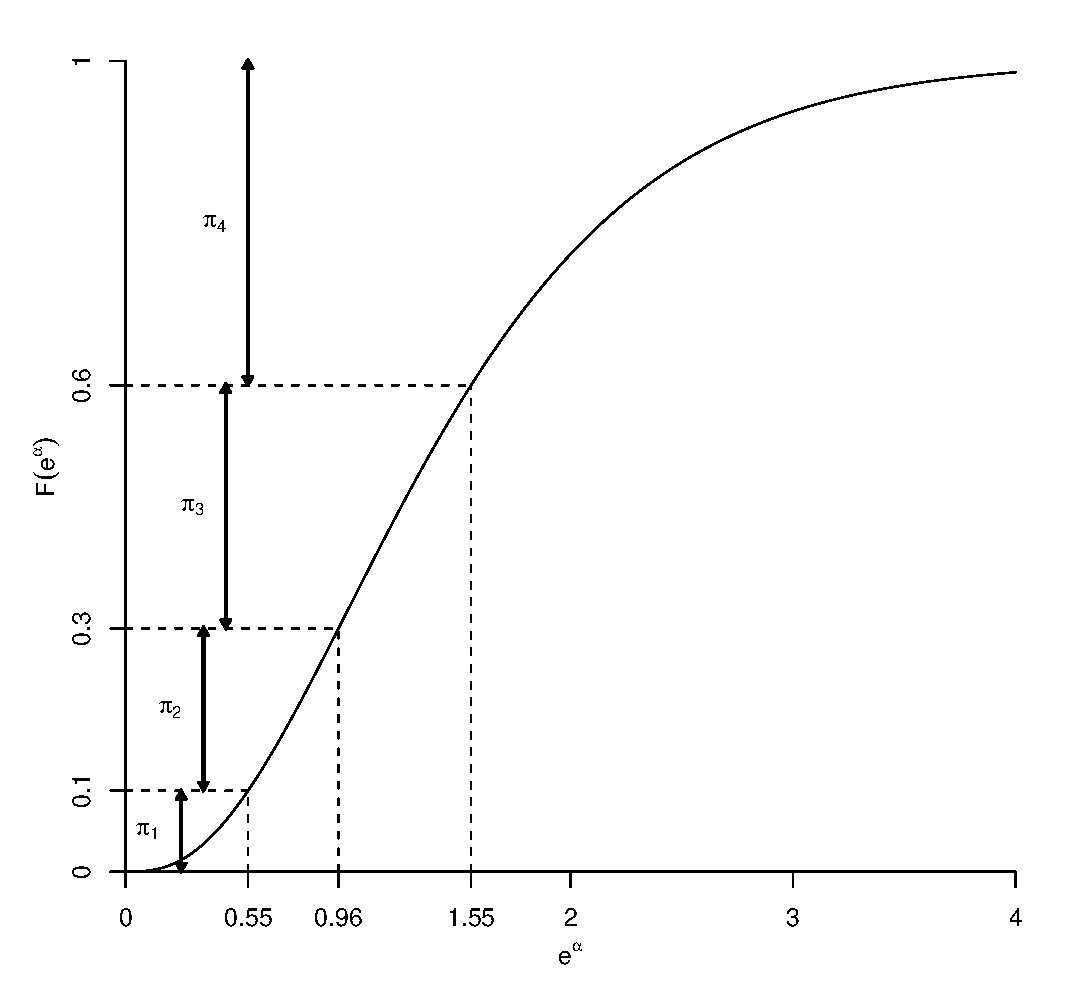
\includegraphics[width=4in]{mix/figs/pidia.pdf}
\caption{Illustration of the parameterisation of the $\pi_j$s. The black curve is a Gamma CDF (with shape parameter 3 and scale parameter 1/2). Here $\bm{\pi}=c(0.1,0.2,0.3,0.4)$. The differences in the ``heights'' of the evaluations of the CDF give the values of $\pi_j$.}
\label{dlbpi}
\end{figure}

\subsubsection{Inverse transform}
To transform from the $\pi_j$s back to the $\alpha_j$s we simply re-arrange the above expression.
\begin{align*}
\pi_j &= F(\sum_{k=1}^j e^{\alpha_k}) - F(\sum_{k=1}^{j-1} e^{\alpha_k})\\
F(\sum_{k=1}^j e^{\alpha_k}) &= \pi_j + F(\sum_{k=1}^{j-1} e^{\alpha_k})\\
\sum_{k=1}^j e^{\alpha_k} &= F^{-1}(\pi_j + F(\sum_{k=1}^{j-1} e^{\alpha_k}))\\
e^{\alpha_j} &= F^{-1}\Big(\pi_j + F(\sum_{k=1}^{j-1} e^{\alpha_k})\Big) - \sum_{k=1}^{j-1} e^{\alpha_k}\\
\alpha_j &= \log_e \Big(F^{-1}\Big(\pi_j + F(\sum_{k=1}^{j-1} e^{\alpha_k})\Big) - \sum_{k=1}^{j-1} e^{\alpha_k}\Big)
\end{align*}
Thus, it is possible to move between the two parametrisations easily.

\subsection{Fitting}
It is well known that mixture model likelihoods are notoriously multi-modal (\cite{BDA} PAGES).

MORE BLURB

Three different strategies were used for the optimisation and offered in the \texttt{mmds} package. The justification being that if one method fails to fit a particular model, then perhaps another might be better at tackling that particular problem. The first and simplest of these methods was a straightforward quasi-Newton method, BFGS (\cite{bfgs}) which simply maximised the likelihood with the help of analytic gradients (see appendix \ref{appendix-mmds-derivs}). In testing this method was unsatisfactory so two other procedures were also developed.

\subsection{BFGS+SANN}
The starting value calculation (see section \ref{mmds-starting-vals}) is relatively primitive and therefore perhaps does not start the optimisation in a particularly good position to begin the maximisation. Given this and the rather complex likelihood, the odds are not stacked in the favour of the optimisation procedure being successful. In order to move around the parameter space, simulated annealing (SIMULATED ANNEALING REF: NUM RECIPES?) is used to begin the maximisation then followed up with a BFGS step to find the maxima. Both BFGS and simulated annealing are available via the \texttt{optim()} function in the base \textsf{R} distribution.

In particular, simulated annealing is used for 250 iterations, then unconstrained BFGS after that. In an attempt to avoid local maxima, these two steps are looped for five iterations and the results stored. The model with the lowest AIC is then chosen from these. If no models fit in the first 5 iterations, the procedure continues until at least one model fits, or there have been 20 attempts at fitting, whichever comes first.

It is worth noting that the method may appear to fail to converge for all attempts, however this does not necessarily indicate that the model will never converge. The stochastic nature of simulated annealing means that it is entirely possible that further runs may yield a useful result.

\subsection{Expectation-Maximisation Algorithm}
A common (CITE SOME PAPERS) way of fitting mixture models is to use the Expectation-Maximisation (EM) algorithm of CITE THE EM PAPER.

First note that the likelihood for mixture models tends to be of the form:

this form appears to be a weighted likelihood... SAY MORE FROM THE PIATER DOC

Outline of the EM algorithm is taken from the very helpful set of notes by \cite{piater}. As is usual with EM, we loop between expectation and maximisation steps until convergence. For brevity we define:
\begin{equation*}
f_j(x_i,zj;\sigma_j) =  \frac{g_j(x_i, zj;\sigma_j)}{\mu_j(zj)},
\end{equation*}
in the line transect case and
\begin{equation*}
f_j(x_i,zj;\sigma_j) = \frac{2 \pi r_i g_j(r_i, zj;\sigma_j)}{nuj}.
\end{equation*}
for the point transect case.

\begin{itemize}
\item \textbf{Expectation}

In the expectation step we need to calculate the expected values of the $w_{ij}$ for each datum $i$ and mixture $j$,
\begin{equation*}
\mathbb{E}[w_{ij}] = \frac{\pi_j f_j(x_i,zj;\sigma_j)}{\sum_{k=1}^J \pi_k f_k(x_i,zj;\sigma_k)},
\end{equation*}
then calculate the $\pi_j$s as:
\begin{equation*}
\pi_j=\frac{1}{n} \sum_{i=1}^n w_{ij}.
\end{equation*}

\item \textbf{Maximisation}

Keeping the $\pi_j$s fixed, optimise with respect to the $\sigma_j$s (or, rather, $\beta_{jk}$s). Here we just use BFGS in \texttt{optim()}. 
\end{itemize}



cite EM/CEM/SEM paper

gelman multimodality

maybe show why other parametrisation doesn't work??


\subsection{Starting values}
\label{mmds-starting-vals}
Starting values are calculated by first sorting data by distance and then dividing it into $k$ equal parts (for a $k$ point mixture). For each of these parts work out a \cite{beavers98}-type estimate of the $\beta_{jk}$s and use that as start point. 

The Beavers and Ramsay estimate is given as the results of running an intercept only regression on $\log(x+\frac{w}{1000})$ (where $w$ denotes the truncation distance, as above) for the non-covariate models. For covariate models, the equation for the $\sigma_j$ is used. The estimated parameters from the linear regression are used as the starting values for the $\beta_{jk}s$.

For the $\alpha_j$s, a set of $\pi_j$ are generated as $1/k$ and then transformed by the procedure above to be on the $\alpha_j$ scale.



\subsection{Derivatives}
[[Maybe this is better as an appendix?]]


%%%%%%%%%%%%%%%%%%%%%%%%%%%%%%%%%%%%%%%%%%%%%%%%%%%
\section{Testing}

\subsection{Simulations}

METRICS

WHY are we doing each of these.

DISCUSSION OF (in particular)

nocovar sim 5

covar with 3pt - what's going on?

3pt with 2pt - what's going on

\subsection{Real data}

Just source in the .tex from the vignette?




%%%%%%%%%%%%%%%%%%%%%%%%%%%%%%%%%%%%%%%%%%%%%%%%%%%
\section{Conclusion}


\section{Acknowledgements}
DLB - pi parametrisation
JLL/Steve/Eric - general comments
Marc - interesting chat
Len - obviously





% start the appendices
\appendix

\chapter{Properties of the within-area distance algorithm}

%%
\label{chap-WAD}


Here some properties of the algorithm given in \secref{mdsdist} are given.

\section{Preliminaries}

To begin with some preliminaries. Notation is as in \secref{mdsdist}, but is refreshed here. In this section a proof of the uniqueness of the shortest path in a simple polygon is given.

\subsection{Notation}

DEFINE everything here: COMBINE!

$p_1$ and $p_2$ always refer to the two points that we want to find the shortest path between

$\Gamma$ is the polygon that we are interested in

$v_i$ refers to a point in a path within the domain, it may or may not be a vertex of $\Gamma$.

$\mathcal{P}_1$ and $\mathcal{P}_2$ are the initial paths between $p_1$ and $p_2$ that trace the boundary.

$\mathcal{P}$ is the working path between $p_1$ and $p_2$.


$\mathcal{S}_{i}$ is a section of a path.

\subsection{Terminology}

The word triangle here is used to refer to the case in which three points, $(v_i,v_{i+1},v_{i+2})$ are vertices of a triangle all the adges of which lie within $\Gamma$. These are the cases in which the DELETE would simplify $(v_i,v_{i+1},v_{i+2})$ to $(v_i,v_{i+2})$.


\subsection{Uniqueness of shortest path}
\label{app-unique-sp}
Propostition: here is one, unique shortest path in a simple polygon (ie. the polygon has no holes).
This is simple to see since if the shortest path were non-unique then there would exist $\mathcal{P}_A$ and  $\mathcal{P}_B$ which were both shortest paths between $p_1$ and $p_2$. It would then be the case there there would be two points $v_1^*$ and $v_2^*$ say where the paths started to differ and ended differing (these could be $p_1$ and $p_2$): the points at which $\mathcal{P}_A$ and  $\mathcal{P}_B$ become disjoint. Call the two paths that lie between $v_1^*$ and $v_2^*$ $\mathcal{S}_{AB}$ and $\mathcal{S}_{BA}$. 

Joining up $\mathcal{S}_{AB}$ and $\mathcal{S}_{BA}$ at $v_1^*$ and $v_2^*$ forms a loop, $\mathcal{L}$, say. There is nothing in the middle of $\mathcal{L}$ (since $\Gamma$ has no holes), in which case there must be a kink in at least one of the paths (since they are not identical, at least one of them must not be a straight line between $v_1^*$ and $v_2^*$), this means that there is a triangle in (at least) one of the paths, which can be straightened ($\mathcal{L}$ does not contain any obstacle stopping this) so the path is not a shortest path and can be shortened. This is a contradiction, therefore the shortest path must be unique.

This proof was adapted from the one given in lecture notes by Leonidas Guibas available at \url{http://graphics.stanford.edu/courses/cs268-09-winter/}.


\section{Properties}

\subsection{The algorithm terminates}

The condition to be fulfilled for the algorithm to terminate is that in two consecutive runs the path does not change, so the first step is to check that it is possible for this to happen, then to move on to show that it always happens. 

Since the ALTER step can act as (a less efficient) DELETE step (since $\mathcal{P}_{ID}$ could just be the straight line between two points, the DELETE substep of the ALTER just removing all of the unecessary vertices and $(v_i,v_{i+1},v_{i+2})$ is then replaced with $(v_i,v_{i+2})$), we only need to consider the ALTER step.

For the algorithm to fail to terminate, the ALTER step would have to create a situation in which one ALTER step would take the path $\mathcal{P}_1^*$ (say) and alter it to be $\mathcal{P}_2^*$ such that the next ALTER step would revert $\mathcal{P}_2^*$ back to $\mathcal{P}_1^*$, these two steps would then continue indefinitely.

If this were to happen it would imply that both $\mathcal{P}_2^*$ was shorter than $\mathcal{P}_1^*$ and $\mathcal{P}_1^*$ was shorter than $\mathcal{P}_2^*$ and since in the ALTER step the $\mathcal{P}_{ID}$ must be shorter than $(v_i,v_{i+1},v_{i+2})$ (not equal in length) then this cannot happen.

Clearly the algorithm cannot continue shortening the path forever, at some point there will be no more shorter routes proposed by the ALTER step and hence it will terminate.


\subsection{The algorithm terminates at the shortest path}

Consider the two initial paths following the boundary, $\mathcal{P}_1$ or $\mathcal{P}_2$ above. Without loss of generality, let $\mathcal{P}_1$ be the shorter of the two initial paths. The DELETE and ALTER steps can be thought of as refining one of these starting paths.

We can think of $\mathcal{P}_1$ as traversing a series of features of the boundary and we would like to include as few of them as possible to obtain the shortest path. The features fall into two classes, they are concave and convex. The names are given as they would appear to one traversing them from inside the domain, so they appear to be opposite to the definitions as used to describe polygons. Concave features extrude from the polygon (ie. they would look like ``caves'' to those traversing the boundary) and convex features intrude into the polygon (ie. they would look like ``mountains'' to those traversing the boundary).




Concave features consist of a set of vertices $(v_i, v_{i+1},\cdots,v_{i+k})$, where all of the vertices between $v_i$ and $v_{i+k}$ can be removed without any of the path falling outside of the domain, one can think of this as capping the top of a hole. Convex features consist of a series of vertices where  only some of the 


The shortest path through a concave section can always be found in a series of DELETE steps: if the concave section alone is taken and triangulated, the DELETE step will always be able to remove all of the vertices in the concave section (since it can be triangulated). This leaves only the starting and ending vertices. Figure \ref{app-WAD-concave} shows how the triangulation removes the vertices.


TKTKTK diagram

Having removed all of the concave parts of the path, this leaves only convex features. In order to find the shortest path around them we can simply trace them (they cannot be reduced any further since they are already convex). It might then be the case that by tracing these convex features further convex and concave features are introduced, however these can be addressed in the next iteration.

The only thing it remains to consider is the points at which the convex segment joins the rest of the path, these may be shortened by using the DELETE step if necessary.

Given that the initial path many consist of only these two elements and that they are removed by the consecutive steps of DELETE and ALTER (obviously there may need to be micro steps of these within each step due to the aforementioned embeddding of caves-within-mountains and mountains-within-caves) we can conclude that the path is the shortest path.

CAN WE?!?!?!?!?!

\subsection{The computational complexity of the algorithm}








\chapter{Derivatives of the likelihood for mixture model detection functions}

% mixture derivatives!
\label{app-mixderivs}

% error function
\newcommand{\erf}{\text{Erf}}
% derivative shortcuts
\newcommand{\palphaj}{\frac{\partial}{\partial \alpha_{j*}}}
\newcommand{\pbetajk}{\frac{\partial}{\partial \beta_{j*k*}}}
%nu_j shortcut + starred
\newcommand{\nuj}{\nu_j(\bm{z}^{(j)})}
\newcommand{\nujs}{\nu_{j*}(\bm{z}^{(j*)})}
% z_ik^j shortcut + with starts
\newcommand{\zijk}{z_{ik}^{(j)}}
\newcommand{\zijkss}{z_{ik*}^{(j*)}}
% z^(j) shortcut + with starts
\newcommand{\zj}{\bm{z}_j}
\newcommand{\zjs}{\bm{z}_{j*}}
% z^(J) shortcut + with starts
\newcommand{\zJ}{\bm{z}_J}

\section{Line transects - likelihood and derivatives}

The likelihood and its derivatives for the covariate case are derived fully below, along with summary results for the non-covariate case (since this is just a special case of the covariate model anyway).

\subsection{The likelihood}

In its full ``natural'' parameterisation (i.e. in terms of $\sigma$s and $\pi$s) the likelihood is given as:
\begin{align*}
\mathcal{L}(\bm{\sigma},\bm{\pi}; \bm{x}, Z) &= \prod_{i=1}^n \sum_{j=1}^J \pi_j \frac{g_j(x_i; \sigma_j(Z;\bm{\beta}_j))}{\mu_j(Z)}.
\end{align*}
That is, the product of the PDF evaluated at each datum, where the PDF is a scaled sum of detection functions divided by the effective strip width (see below). 

The $\log$-likelihood is then:
\begin{align*}
l(\bm{\sigma},\bm{\pi}; \bm{x}, Z) &= \sum_{i=1}^n \log\Big(\sum_{j=1}^J \pi_j \frac{g_j(x_i;\sigma_j(Z;\bm{\beta}_j))}{\mu_j(Z)}\Big)
\end{align*}
The effective strip (half-)width, $\mu_j(\bm{z})$, is defined as:
\begin{align*}
\mu_j(\bm{z})=& \int_0^w g_j(x;\sigma_j(\bm{z};\bm{\beta}_j)) \text{d}x.
\end{align*}
where $w$ is the truncation distance (after which recorded distances are discarded). $\mu_j(\bm{z})$ is an $n$-vector. In the case where there are no covariates we can write:
\begin{align*}
\mu_j=& \int_0^w g_j(x;\sigma_j) \text{d}x.
\end{align*}
$\mu_j$ is a scalar.
In order to be as general as possible, the covariate case is considered throughout.

As mentioned above, we consider the case in which we only have one observation and associates covariates. We can then write the $\log$-likelihood as:
\begin{align*}
l(\bm{\sigma},\bm{\pi}; x, \bm{z}) &= \log\Big(\sum_{j=1}^J \pi_j \frac{g_j(x;\sigma_j(\bm{z};\bm{\beta}_j))}{\mu_j(\bm{z})}\Big),
\end{align*}
using exactly the same notation as above. This is used as the starting point for all derivative calculations below.


\subsubsection{Mixture proportions}


To find the derivatives with respect to the mixture proportions, first reparameterise in terms of $\alpha_j$s (for simplicity $\bm{\sigma}$ is left as-is). The derivative of $l(\bm{\sigma},\bm{\alpha};x, \bm{z})$ with respect to some $\alpha_{j*}$ is given as
\begin{align*}
\frac{\partial l(\bm{\sigma},\bm{\alpha}; x, \bm{z})}{\partial \alpha_{j*}} &= \palphaj \log\Big(\sum_{j=1}^J \pi_j \frac{g_j(x;\sigma_j)}{\mu_j(\bm{z})}\Big),\\
&= \frac{\palphaj \Big(\sum_{j=1}^J \pi_j \frac{g_j(x;\sigma_j)}{\mu_j(\bm{z})}\Big)}{\Big(\sum_{j=1}^J \pi_j \frac{g_j(x;\sigma_j)}{\mu_j(\bm{z})}\Big)}.
\end{align*}
Letting
\begin{align*}
\mathcal{F}(x, \bm{z};\bm{\sigma},\bm{\pi})=\sum_{j=1}^J \pi_j \frac{g_j(x;\sigma_j)}{\mu_j(\bm{z})}
\end{align*}
we can write:
\begin{align*}
\frac{\partial l(\bm{\sigma},\bm{\alpha};x,\bm{z})}{\partial \alpha_{j*}} &= \frac{1}{\mathcal{F}(x,\bm{z} ;\bm{\sigma},\bm{\alpha})} \palphaj \Big(\sum_{j=1}^J \pi_j \frac{g_j(x;\sigma_j)}{\mu_j(\bm{z})}\Big)\\
&= \frac{1}{\mathcal{F}(x, \bm{z};\bm{\sigma},\bm{\alpha})} \palphaj \Big( \sum_{j=1}^{J-1}\pi_j \frac{g_j(x; \sigma_j)}{\mu_j(\bm{z})} + \Big(1-\sum_{j=1}^{J-1}\pi_j \Big) \frac{g_J(x;\sigma_J)}{\mu_J(\bm{z})}\Big)
\end{align*}
Now, we know that the relation between $\pi_{j*}$ and $\alpha_{j*}$ is
\begin{align*}
\pi_j = F(\sum_{k=1}^j e^{\alpha_k}) - F(\sum_{k=1}^{j-1} e^{\alpha_k}),
\end{align*}
so, substituting this in we obtain
\begin{align*}
\frac{\partial l(\bm{\sigma},\bm{\alpha};x,\bm{z})}{\partial \alpha_{j*}} &= \frac{1}{\mathcal{F}(x, \bm{z};\bm{\sigma},\bm{\alpha})} \palphaj \Big\{ \sum_{j=1}^{J-1} [F(\sum_{k=1}^j e^{\alpha_k}) - F(\sum_{k=1}^{j-1} e^{\alpha_k})] \frac{g_j(x;\sigma_j)}{\mu_j(\bm{z})} +\\
& \qquad \Big[1-\sum_{j=1}^{J-1}(F(\sum_{k=1}^j e^{\alpha_k}) - F(\sum_{k=1}^{j-1} e^{\alpha_k})) \Big] \frac{g_J(x_i;\sigma_J)}{\mu_J(\bm{z})}\Big\}\\
&= \sum_{i=1}^n \frac{1}{\mathcal{F}(x, \bm{z};\bm{\sigma},\bm{\alpha})} \Big\{ \sum_{j=1}^{J-1} \Big[\palphaj F(\sum_{k=1}^j e^{\alpha_k}) - \palphaj F(\sum_{k=1}^{j-1} e^{\alpha_k})\Big] \frac{g_j(x;\sigma_j)}{\mu_j(\bm{z})} \\
&\qquad -\Big[\sum_{j=1}^{J-1} (\palphaj F(\sum_{k=1}^j e^{\alpha_k}) - \palphaj F(\sum_{k=1}^{j-1} e^{\alpha_k})\Big] \frac{g_J(x;\sigma_J)}{\mu_J(\bm{z})}\Big\}.
\end{align*}
Looking at the derivative terms in the above expression:
\begin{equation*}
\palphaj F(\sum_{k=1}^j e^{\alpha_k})=A_{j}=\begin{cases}
e^{\alpha_{j*}}f(\sum_{k=1}^j e^{\alpha_k})& \text{for $j\geq j*$},\\
0 & \text{for $j<j*$}.
\end{cases}
\end{equation*}
and
\begin{equation*}
\palphaj F(\sum_{k=1}^{j-1} e^{\alpha_k})=A_{(j-1)}=\begin{cases}
e^{\alpha_{j*}}f(\sum_{k=1}^{j-1} e^{\alpha_k})& \text{for $j-1\geq j*$},\\
0 & \text{for $j-1<j*$}.
\end{cases}
\end{equation*}
\begin{align*}
\frac{\partial l(\bm{\sigma},\bm{\alpha}; x,\bm{z})}{\partial \alpha_{j*}} &= \frac{1}{\mathcal{F}(x, \bm{z};\bm{\sigma},\bm{\alpha})} \Big\{ \Big[\sum_{j=1}^{J-1} (A_{j}-A_{(j-1)}) \frac{g_j(x;\sigma_j)}{\mu_j(\bm{z})}\Big] - \sum_{j=1}^{J-1}\Big[ (A_{j}-A_{(j-1)})\frac{g_J(x;\sigma_J)}{\mu_J(\bm{z})} \Big]\Big\},\\%.
&= \frac{1}{\mathcal{F}(x, \bm{z};\bm{\sigma},\bm{\alpha})} \sum_{j=1}^{J-1} (A_{j}-A_{(j-1)}) \frac{g_j(x;\sigma_j)}{\mu_j(\bm{z})}-(A_{j}-A_{(j-1)})\frac{g_J(x;\sigma_J)}{\mu_J(\bm{z})},\\
&= \frac{1}{\mathcal{F}(x, \bm{z};\bm{\sigma},\bm{\alpha})} \sum_{j=1}^{J-1} (A_{j}-A_{(j-1)}) \Big(\frac{g_j(x;\sigma_j)}{\mu_j(\bm{z})}-\frac{g_J(x;\sigma_J)}{\mu_J(\bm{z})} \Big).
\end{align*}
Finally, when there are multiple observations (summing over $i$) and writing out the likelihood in full, we have:
\begin{align*}
\frac{\partial l(\bm{\sigma},\bm{\alpha}; \bm{x},Z)}{\partial \alpha_{j*}} &= \sum_{i=1}^n \frac{1}{\mathcal{F}(x_i, Z;\bm{\sigma},\bm{\alpha})} \sum_{j=1}^{J-1} (A_{j}-A_{(j-1)}) \Big( \frac{g_j(x_i;\sigma_j(Z;\bm{\beta_j}))}{\mu_j(Z)} - \frac{g_J(x_i;\sigma_J(Z;\bm{\beta_J}))}{\mu_J(Z)} \Big).
\end{align*}

Note that we never take derivatives with respect to $\alpha_J$.


%%%%%%%%%%%%%%%%%%%%%%%%%%%%%%%%%%%%%%%%%%%%%%%%%%%%%%%%%%%
\subsubsection{Detection function parameters}

Now to find derivatives with respect to $\beta_{j*k*}$, using the expression for the log-likelihood and adopting the same approach of not using the parametrisation until absolutely necessary, as above...
\begin{align*}
\frac{\partial l(\bm{\sigma},\bm{\pi};x, \bm{z})}{\partial \beta_{j*k*}} &= \pbetajk \log\Big(\sum_{j=1}^J \pi_j \frac{g_j(x;\sigma_j)}{\mu_j(\bm{z})}\Big),\\
&= \frac{1}{\mathcal{F}(x,\bm{z};\bm{\sigma},\bm{\pi})} \pbetajk \sum_{j=1}^J \pi_j \frac{g_j(x;\sigma_{j})}{\mu_j(\bm{z})},\\
&= \frac{1}{\mathcal{F}(x,\bm{z};\bm{\sigma},\bm{\pi})} \pbetajk \pi_{j*} \frac{g_{j*}(x;\sigma_{j*})}{\mu_{j^*}(\bm{z})},\\
&= \frac{\pi_{j*}}{\mathcal{F}(x,\bm{z};\bm{\sigma},\bm{\pi})} \frac{\pbetajk g_{j*}(x,\bm{z};\sigma_{j*}) \mu_{j^*}(\bm{z}) - g_{j*}(x;\sigma_{j*}) \pbetajk \mu_{j^*}(\bm{z})}{[\mu_{j^*}(\bm{z})]^2}.\\
\end{align*}
Taking this expression bit-by-bit and finding the derivative terms that we need, first: $\frac{\partial g_{j*}(x;\sigma_{j*})}{\partial \beta_{j*k*}}$:
\begin{align*}
\frac{\partial g_{j*}(x;\sigma_{j*})}{\partial \beta_{j*k*}} &= \pbetajk \exp\Big( -\frac{x_i^2}{2\sigma_{j*}^2} \Big)
\end{align*}
Applying the chain rule, since $\sigma_{j*}$ is a function of the $\beta_{jk}$s:
\begin{align*}
\frac{\partial \sigma_{j*}(\bm{z};\bm{\beta}_{j*})}{\partial \beta_{j*k*}} &= \pbetajk\exp \Big( \beta_{0j} + \sum_{k\in K_j} z_k \beta_{j*k}\Big),\\
&= z_{k*} \exp \Big( \beta_{0j} + \sum_{k \in K_j} z_{k} \beta_{j*k}\Big),\\
&= z_{k*}\sigma_{j*}(\bm{z};\bm{\beta}_{j*}) = z^{(j*)}_{ik*}\sigma_{j*}.
\end{align*}
Hence:
\begin{align*}
 \frac{\partial}{\partial \beta_{j*k*}} \exp\Big( -\frac{x^2}{2\sigma_{j*}^2} \Big) &=  \pbetajk \exp\Big( -\frac{x^2}{2\sigma_{j*}^2} \Big)  \frac{\partial \sigma_{j*}}{\partial \beta_{j*k*}}\\
&= z_{k*} \Big( \frac{x}{\sigma_{j*}}\Big)^2 \exp \Big(-\frac{x^2}{2 \sigma_{j*}^2}\Big) 
\end{align*}
$\mu_{j*}(\bm{z})$ can be expressed in terms of the error function...
\begin{align*}
\frac{\partial \mu_{j*}(\bm{z})}{\partial \beta_{j*k*}} &=\pbetajk \Big( \sqrt{\frac{\pi}{2}} \sigma_{j*} \erf\Big(\frac{w}{\sqrt{2\sigma_{j*}^2}}\Big) \Big)\\
&= \erf\Big(\frac{w}{\sqrt{2\sigma_{j*}^2}}\Big) \pbetajk \Big( \sqrt{\frac{\pi}{2}} \sigma_{j*} \Big) + \sqrt{\frac{\pi}{2}} \sigma_{j*} \pbetajk \Big(\erf\Big(\frac{w}{\sqrt{2\sigma_{j*}^2}}\Big) \Big)
\end{align*}
To find $\frac{\partial}{\partial \beta_{j*k*}} \erf\Big(\frac{w}{\sqrt{2\sigma_{j*}^2}}\Big)$, note that we can write:
\begin{align*}
\frac{\partial}{\partial \beta_{j*k*}} \erf\Big(\frac{w}{\sqrt{2\sigma_{j*}^2}}\Big) = \frac{\partial}{\partial \beta_{j*k*}} S(u(\sigma_{j*}(\bm{z};\bm{\beta}_{j*})))
\end{align*}
where $\bm{\beta}_{j*}$ contains all the necessary coefficients for that mixture part. Turning the handle on the chain rule sausage machine gives:
\begin{align*}
\frac{\partial}{\partial \beta_{j*k*}} S(u(\sigma_{j*}(\bm{z};\bm{\beta}_{j*}))) = \frac{\partial S(u)}{\partial u} \frac{\partial u(\sigma_{j*})}{\partial \sigma_{j*} } \frac{\partial \sigma_{j*}(\bm{z};\bm{\beta}_{j*})}{\partial \beta_{j*k*}}
\end{align*}
where 
\begin{align*}
S(u) = \int_0^{u} \exp(-t^2) \text{d}t \quad \text{and} \quad u(\sigma_{j*})=\frac{w}{\sqrt{2\sigma_{j*}^2}}.
\end{align*}
Their derivatives being
\begin{align*}
\frac{\partial S(u)}{\partial u} = \frac{2}{\sqrt{\pi}} \exp(-u^2) \text{,} \quad \frac{\partial u(\sigma_{j*})}{\partial \sigma_{j*}} = -\frac{w}{\sqrt{2}}\sigma_{j*}^{-2},
\end{align*}
and $\frac{\partial \sigma_{j*}}{\partial \beta_{j*k*}}$ from above.

Given these terms, it's just a case of multiplying them:
\begin{align*}
\frac{\partial S(u)}{\partial u} \frac{\partial u(\sigma_{j*})}{\partial \sigma_{j*} } \frac{\partial \sigma_{j*}(\bm{\beta}_{j*})}{\partial \beta_{j*k*}} = - \sqrt{\frac{2}{\pi}} \frac{w z_{k*}}{\sigma_{j*}} \exp\Big( -\frac{w^2}{2\sigma_{j*}^2} \Big)
\end{align*}
Rolling that up:
\begin{align*}
\frac{\partial \mu_{j*}(\bm{z})}{\partial \beta_{j*k*}} &= \sqrt{\frac{\pi}{2}} \erf\Big(\frac{w}{\sqrt{2\sigma_{j*}^2}}\Big) z_{k*} \sigma_{j*}  +  \Big( - \frac{w z_{k*} }{\sigma_{j*}} \exp\Big( -\frac{w^2}{2\sigma_{j*}^2} \Big) \Big)\\
&= \mu_{j*}(\bm{z}) z_{k*} - w z_{k*} \exp\Big( -\frac{w^2}{2\sigma_{j*}^2} \Big)\\
&= z_{k*} \Big(\mu_{j*}(\bm{z}) - w \exp\Big( -\frac{w^2}{2\sigma_{j*}^2} \Big)\Big)
\end{align*}
Finally, putting that all back into the quotient rule,
\begin{align*}
\frac{\partial l(\bm{\sigma},\bm{\pi}; x, \bm{z})}{\partial \beta_{j*k*}} &= \frac{\pi_{j*}}{\mathcal{F}(x,\bm{z};\bm{\sigma},\bm{\pi})} \frac{\frac{\partial}{\partial \beta_{j*k*}} g_{j*}(x;\sigma_{j*}) \mu_{j^*}(\bm{z}) - g_{j*}(x;\sigma_{j*})\frac{\partial}{\partial \beta_{j*k*}} \mu_{j^*}(\bm{z})}{(\mu_{j^*}(\bm{z}))^2},\\
&= \frac{\pi_{j*}}{\mathcal{F}(x,\bm{z};\bm{\sigma},\bm{\pi})} \frac{ z_{k*} \Big( \frac{x}{\sigma_{j*}}\Big)^2 \exp \Big(-\frac{x^2}{2 \sigma_{j*}^2}\Big)  \mu_{j^*}(\bm{z}) - \exp \Big(-\frac{x^2}{2 \sigma_{j*}^2}\Big) z_{k*} \Big(\mu_{j*}(\bm{z}) - w \exp\Big( -\frac{w^2}{2\sigma_{j*}^2} \Big)\Big) }{(\mu_{j^*}(\bm{z}))^2},\\
&= \frac{\pi_{j*} z_{k*}}{(\mu_{j^*}(\bm{z}))^2\mathcal{F}(x,\bm{z};\bm{\sigma},\bm{\pi})} \exp \Big(-\frac{x^2}{2 \sigma_{j*}^2}\Big) \Big[\Big( \frac{x}{\sigma_{j*}}\Big)^2 \mu_{j^*}(\bm{z}) - \mu_{j*}(\bm{z}) + w \exp\Big( -\frac{w^2}{2\sigma_{j*}^2}\Big)\Big],\\
&= \frac{\pi_{j*} z_{k*}}{\mu_{j^*}(\bm{z})\mathcal{F}(x,\bm{z};\bm{\sigma},\bm{\pi})} \exp \Big(-\frac{x^2}{2 \sigma_{j*}^2}\Big) \Big[\Big( \frac{x}{\sigma_{j*}}\Big)^2  + \frac{w}{\mu_{j^*}(\bm{z})} \exp\Big( -\frac{w^2}{2\sigma_{j*}^2}\Big) -1\Big].
\end{align*}

Now writing this out in full, for multiple observations, as in the mixture proportion case:
\begin{align*}
\frac{\partial l(\bm{\sigma},\bm{\pi}; \bm{x}, Z)}{\partial \beta_{j*k*}} &= \sum_{i=1}^n \frac{\pi_{j*} z_{ik*}}{\mu_{j^*}(Z)\mathcal{F}(x_i,Z;\bm{\sigma},\bm{\pi})} \exp \Big(-\frac{x_i^2}{2 \sigma_{j*}(Z,\bm{\beta}_{j*})^2}\Big) \Big[\Big( \frac{x_i}{\sigma_{j*}(Z,\bm{\beta_}{j*})}\Big)^2\\
&  + \frac{w}{\mu_{j^*}(Z)} \exp\Big( -\frac{w^2}{2\sigma_{j*}(Z,\bm{\beta}_{j*})^2}\Big) -1\Big].
\end{align*}

Note that for the non-covariate case, $z_{ik*}=1 \text{ } \forall i, k^*=1$ and $\mu_{j^*}(\bm{z})$ is replaced with $\mu_{j^*}$. Other than that, the expressions are identical.

%%%%%%%%%%%%%%%%%%%%%%%%%%%%%%%%%%%%%%%%%%%

\section{Point transects - likelihood and derivatives}

As above, the likelihood and its derivatives for the covariate case are derived fully below, along with summary results for the non-covariate case (since this is just a special case of the covariate model anyway).

\subsection{The likelihood}

Again looking at the likelihood in its ``natural'' parameterisation, we have:
\begin{align*}
\mathcal{L}(\bm{r}, \bm{z} ;\bm{\sigma},\bm{\pi}) &= \prod_{i=1}^n \sum_{j=1}^J \pi_j \frac{2 \pi r_i g_j(r_i, \zijk;\sigma_j)}{\nuj}.
\end{align*}
So, the $\log$-likelihood is:
\begin{align*}
l(\bm{r}, \bm{z};\bm{\sigma},\bm{\pi}) &= \sum_{i=1}^n \log\Big(\sum_{j=1}^J \pi_j \frac{r_i g_j(r_i,\zijk;\sigma_j)}{\nuj}\Big)
\end{align*}
Again,the $\bm{\sigma}$ and $\bm{\pi}$ vectors are only proxies for $\bm{\beta}$ and $\bm{\alpha}$, used in the optimisation parameterisation.

Here $\nuj$ is defined similarly to $\mu_j(\bm{z}^{(j)})$, above,
\begin{align*}
\nuj=& \int_0^w 2 \pi r g_j(r,\bm{z}^{(j)};\sigma_j) \text{d}r,\\
&= 2 \pi \sigma_j^2 \Big[1-\exp\Big( -\frac{w^2}{2\sigma_j^2}\Big)\Big],
\end{align*}

Note that the likelihood is essentially the same as the line transect case, but the detection function is multiplied by a factor of $2 \pi r$.


\subsubsection{Mixture proportions}

The derivatives with respect to the mixture proportions, are exactly as above, aside from the additional $r_i$ term as above.


\subsubsection{Detection function parameters}

As above, assume that we have a covariate model and that the non-covariate case is just a special case of that.
\begin{align*}
\frac{\partial l(\bm{r}, \bm{z};\bm{\theta},\bm{\pi})}{\partial \beta_{j*k*}} &= \pbetajk \sum_{i=1}^n \log\Big(\sum_{j=1}^J \pi_j \frac{2 \pi r_i g_j(r_i,\zj;\sigma_j)}{\nuj}\Big),\\
&= \sum_{i=1}^n \pbetajk \log\Big(\sum_{j=1}^J \pi_j \frac{2 \pi  r_i g_j(r_i,\zj;\sigma_j)}{\nuj}\Big),\\
&= \sum_{i=1}^n \frac{1}{\mathcal{F}(r_i,\bm{z};\bm{\sigma},\bm{\pi})} \pbetajk \sum_{j=1}^J \pi_j \frac{2 \pi r_i g_j(r_i,\zj;\sigma_{j*})}{\nuj},\\
&= \sum_{i=1}^n \frac{2 \pi  \pi_{j*}}{\mathcal{F}(r_i,\bm{z};\bm{\sigma},\bm{\pi})} \pbetajk \frac{r_i g_{j*}(r_i,\zjs;\sigma_{j*})}{\nujs},\\
\end{align*}
since there is a closed form for $\nuj$ we can write:
\begin{align*}
\frac{\partial l(\bm{r}, \bm{z};\bm{\theta},\bm{\pi})}{\partial \beta_{j*k*}} &= \sum_{i=1}^n \frac{2 \pi \pi_{j*}}{\mathcal{F}(r_i,\bm{z};\bm{\sigma},\bm{\pi})} \pbetajk \frac{r_i \exp( -\frac{r_i^2}{2\sigma_{j*}^2})}{2 \pi \sigma_{j*}^2 (1-\exp( -\frac{w}{2\sigma_{j*}^2}))}.\\
\end{align*}
Then using the quotient rule:
\begin{align*}
\frac{\partial l(\bm{r}, \bm{z};\bm{\theta},\bm{\pi})}{\partial \beta_{j*k*}} &= \sum_{i=1}^n \frac{2 \pi \pi_{j*}}{\mathcal{F}(r_i,\bm{z};\bm{\sigma},\bm{\pi})}\frac{1}{(\nujs)^2} \Big\{  [2 \pi\sigma_{j*}^2(1-\exp( -\frac{w^2}{2\sigma_{j*}^2}))] \pbetajk (r_i \exp( -\frac{r_i^2}{2\sigma_{j*}^2}))\\
&\qquad -r_i \exp( -\frac{r_i^2}{2\sigma_{j*}^2}) \pbetajk [2 \pi\sigma_{j*}^2(1-\exp( -\frac{w^2}{2\sigma_{j*}^2}))]\Big\}.\\
\end{align*}
Taking this bit-by-bit...
\begin{align*}
\pbetajk (r_i \exp( -\frac{r_i^2}{2\sigma_{j*}^2}))&= r_i \exp( -\frac{r_i^2}{2\sigma_{j*}^2})\pbetajk \Big(-\frac{r_i^2}{2\sigma_{j*}^2} \Big),\\
&= r_i \exp( -\frac{r_i^2}{2\sigma_{j*}^2}) \Big(-\frac{r_i^2}{2} \Big) \pbetajk \sigma_{j*}^{-2}.
\end{align*}
Since we are assuming that we can decompose the scale parameter as $\sigma_j = \exp ( \sum_{k=0}^{K} z^{(j)}_{ik} \beta_{jk})$, 
\begin{align*}
\pbetajk \sigma_{j*}^{-2} &= \pbetajk \Big(\exp ( \sum_{k=0}^{K} \zijk \beta_{j*k})\Big)^{-2},\\
&= -2 \zijkss \Big(\exp ( \sum_{k=0}^{K} \zijk \beta_{j*k})\Big)^{-2},\\
&= -2 \zijkss \sigma_{j*}^{-2}.\\
\end{align*}
So,
\begin{equation*}
\pbetajk (r_i \exp\Big( -\frac{r_i^2}{2\sigma_{j*}^2} \Big)) = \zijkss \frac{r_i^3}{\sigma_{j*}^2} \exp\Big( -\frac{r_i^2}{2\sigma_{j*}^2} \Big).
\end{equation*}
Next, $\pbetajk (2 \pi \sigma_{j*}^2(1-\exp( -\frac{w^2}{2\sigma_{j*}^2})))$. Using the product rule,
\begin{equation*}
2 \pi \pbetajk \Big( \sigma_{j*}^2(1-\exp( -\frac{w^2}{2\sigma_{j*}^2})) \Big) = 2\pi \Big[(1-\exp( -\frac{w^2}{2\sigma_{j*}^2}))\pbetajk \sigma_{j*}^2 +  \sigma_{j*}^2 \pbetajk (1-\exp( -\frac{w^2}{2\sigma_{j*}^2}))\Big]
\end{equation*}
Then,
\begin{equation*}
\pbetajk \sigma_{j*}^2=2 \zijkss \sigma_{j*}^2,
\end{equation*}
and the other bit:
\begin{align*}
\pbetajk (1-\exp( -\frac{w^2}{2\sigma_{j*}^2}))&= - \pbetajk \exp( -\frac{w^2}{2\sigma_{j*}^2})\\
&= - \exp( -\frac{w^2}{2\sigma_{j*}^2}) \pbetajk \Big( -\frac{w^2}{2\sigma_{j*}^2}\Big)\\
&= z_{ik*} \Big(\frac{w}{\sigma_{j*}}\Big)^2 \exp( -\frac{w^2}{2\sigma_{j*}^2})
\end{align*}
Putting it all together:
\begin{align*}
2\pi \pbetajk (\sigma_{j*}^2(1-\exp( -\frac{w^2}{2\sigma_{j*}^2})))&= 2\pi \Big[(1-\exp( -\frac{w^2}{2\sigma_{j*}^2})) 2 \zijkss \sigma_{j*}^2 +  \sigma_{j*}^2 \zijk \Big(\frac{w}{\sigma_{j*}}\Big)^2 \exp( -\frac{w^2}{2\sigma_{j*}^2})\Big]\\
&=\zijkss \Big( 2  \nujs +  2\pi w^2 \exp( -\frac{w^2}{2\sigma_{j*}^2})\Big)\\
\end{align*}
Putting all that into the quotient rule:
\begin{align*}
\pbetajk \frac{r_i \exp( -\frac{r_i}{2\sigma_{j*}^2} )}{\sigma_{j*}^2(1-\exp\{ -\frac{w^2}{2\sigma_{j*}^2}\})} &= \frac{1}{[\nujs]^2} \Big\{  \Big[ 2 \pi\sigma_{j*}^2(1-\exp( -\frac{w^2}{2\sigma_{j*}^2}))\Big] \zijkss \frac{r_i^3}{\sigma_{j*}^2} \exp( -\frac{r_i^2}{2\sigma_{j*}^2} )\\
&\qquad -r_i \exp( -\frac{r_i^2}{2\sigma_{j*}^2}) \zijkss \Big[ 2  \nujs +  2\pi w^2 \exp( -\frac{w^2}{2\sigma_{j*}^2})\Big]\Big\},\\
&= \frac{\zijkss r_i \exp(-\frac{r_i^2}{2\sigma_{j*}^2})}{[\nujs]^2} \Big(  \nujs \Big(\frac{r_i}{\sigma_{j*}}\Big)^2 - 2  \nujs +  2\pi w^2 \exp( -\frac{w^2}{2\sigma_{j*}^2})\Big)\\
&= \frac{\zijkss r_i \exp\{ -\frac{r_i^2}{2\sigma_{j*}^2}\}}{\nujs} \Big[ \Big(\frac{r_i}{\sigma_{j*}}\Big)^2 - 2 +  2\pi \frac{w^2}{\nujs} \exp( -\frac{w^2}{2\sigma_{j*}^2})\Big].
\end{align*}
Finally obtaining:
\begin{align*}
\frac{\partial l(\bm{r}, \bm{z};\bm{\sigma},\bm{\pi})}{\partial \beta_{j*k*}} &= \sum_{i=1}^n \frac{2 \pi \pi_{j*}}{\mathcal{F}(r_i,\bm{z};\bm{\sigma},\bm{\pi})} \frac{\zijkss r_i \exp( -\frac{r_i^2}{2\sigma_{j*}^2})}{\nujs} \Big[ \Big(\frac{r_i}{\sigma_{j*}}\Big)^2 - 2 +  2\pi \frac{w^2}{\nujs} \exp( -\frac{w^2}{2\sigma_{j*}^2})\Big].
\end{align*}






\bibliographystyle{chicago}
\bibliography{bib-hell}

% Acknowledgements: Elle, Simon, Len, G+R, parents, all at CREEM (for summer work), Jay ver Hoef? (hah!) Lindesay Scott-Hayward? Jason Matthiopoulos, Jeff Laake


\end{document}
